% xelatex -synctex=1 -interaction=nonstopmode -output-driver="xdvipdfmx -V 5" %.tex

%% Version for one sided printing:
% margins: left 40mm, right 25mm, top and bottom 25mm
% (BUT LaTeX adds automaticly 1in)
% \openright makes following text start on right side of book
%\documentclass[12pt,a4paper]{report}
%\setlength\textwidth{145mm}
%\setlength\textheight{247mm}
%\setlength\oddsidemargin{15mm}
%\setlength\evensidemargin{15mm}
%\setlength\topmargin{0mm}
%\setlength\headsep{0mm}
%\setlength\headheight{0mm}
%\let\openright=\clearpage

%% Version for two sided printing:
\documentclass[12pt,a4paper,twoside,openright]{report}
\setlength\textwidth{145mm}
\setlength\textheight{247mm}
\setlength\oddsidemargin{15mm}
\setlength\evensidemargin{0mm}
\setlength\topmargin{0mm}
\setlength\headsep{0mm}
\setlength\headheight{0mm}
\let\openright=\cleardoublepage

%\usepackage[utf8]{inputenc}
\usepackage[czech,english]{babel}
%\usepackage[T1]{fontenc}
%\usepackage[american]{babel}

\usepackage{fontspec}
\newfontfamily\consolas{Consolas}
%\defaultfontfeatures{Mapping=tex-text}
%\setmonofont{Consolas}
%\usepackage{xunicode}
%\usepackage{xltxtra}


\usepackage{comment}
%\usepackage{setspace}
%\usepackage{parskip}

\usepackage{subfig}
\usepackage{wrapfig}
\usepackage{graphicx}
%\usepackage{amsthm}
\usepackage{booktabs}  % nicer tables
\usepackage[bottom]{footmisc}  % footnotes at the bottom of page

\usepackage[titletoc]{appendix}

\usepackage{tikz}
\usetikzlibrary{positioning,shapes,arrows,trees}
\usetikzlibrary{decorations.pathmorphing} % for snake lines

\tikzstyle{block} = [draw, fill=blue!20, rectangle, minimum height=3em, minimum width=6em]
\tikzstyle{blockx} = [draw, fill=green!20, rectangle, minimum height=3em, minimum width=6em]
\tikzstyle{coord} = [coordinate]
\tikzstyle{snakeline} = [decorate, decoration={pre length=0mm, post length=1mm, snake, amplitude=1mm, segment length=3mm}, ->]


\usepackage[autostyle]{csquotes}
\usepackage{xspace}

\usepackage[
	backend=biber,
	style=alphabetic,
	backref=true,
%	backrefstyle=all+,
	natbib=true,
	url=false,  % url field of @online entries is always printed
	doi=false,
	eprint=false
]{biblatex}
\renewcommand{\labelalphaothers}{*}
\addbibresource{bibliography.bib}

\usepackage{color}
\definecolor{linkClr}{RGB}{64,0,0}  % dark red
\definecolor{citeClr}{RGB}{0,64,0}  % dark green
\definecolor{urlClr}{RGB}{0,0,64}  % dark blue

\usepackage{listings}  % \lstlisting enviroment - source code highliting


\usepackage{syntaxHighlighters}  % needs packages color and listings

\usepackage{hyperref}  % after all other packages
\hypersetup{
	%unicode=true,
	pdftitle=L-systems online,
	pdfauthor=Marek Fišer,
	pdfkeywords={L-system}{generator}{online}{universal}{library},
	colorlinks=true,
	linkcolor=linkClr,
	citecolor=citeClr,
	urlcolor=urlClr
}

%%% Little tweaks

% These macros remove white space above headers of chapters.
\makeatletter
\def\@makechapterhead#1{
  {\parindent \z@ \raggedright \normalfont
   \Huge\bfseries \thechapter. #1
   \par\nobreak
   \vskip 20\p@
}}
\def\@makeschapterhead#1{
  {\parindent \z@ \raggedright \normalfont
   \Huge\bfseries #1
   \par\nobreak
   \vskip 20\p@
}}
\makeatother

% Definition of chapter macro for chapters that are not numbered but they are in TOC.
\def\chapwithtoc#1{
\chapter*{#1}
\addcontentsline{toc}{chapter}{#1}
}

% default path for graphics
\graphicspath{{img/}}

% macros for L-system to avoid hyphenation of it.
\newcommand{\lsystem}{\mbox{L-system}\xspace}
\newcommand{\lsystems}{\mbox{L-systems}\xspace}


% less spavec in lists
\newenvironment{itemize*}
	{\begin{itemize}
		%\setlength{\itemsep}{0pt}
		\setlength{\parskip}{0pt}}
	{\end{itemize}}
\newenvironment{enumerate*}
	{\begin{enumerate}\setlength{\parskip}{0pt}}
	{\end{enumerate}}
\newenvironment{description*}
	{\begin{description}\setlength{\parskip}{0pt}}
	{\end{description}}

% do not break in paragraph
%\widowpenalties 1 10000
\raggedbottom

\renewcommand{\lstlistingname}{Source code}
\renewcommand{\lstlistlistingname}{List of source codes}

% debugging
\includeonly{design}


\begin{document}


\pagestyle{empty}
\begin{center}

\large

Charles University in Prague

\medskip

Faculty of Mathematics and Physics

\vfill

{\bf\Large BACHELOR THESIS}

\vfill

\centerline{\mbox{
\includegraphics[width=60mm]{logo}}}

\vfill
\vspace{5mm}

{\LARGE Marek Fišer}

\vspace{15mm}

% Name of thesis exactly according to the specification.
{\LARGE\bfseries L-systems online}

\vfill

% Official name of department or institute where the work was officially specified.
% (According to Internal Structure of MFF UK)
Department of Software and Computer Science Education

\vfill

\begin{tabular}{rl}

Supervisor of the bachelor thesis: & RNDr. Josef Pelikán \\
\noalign{\vspace{2mm}}
Study program: & Computer Science \\
\noalign{\vspace{2mm}}
Specialization: & Programming \\
\end{tabular}

\vfill

Prague 2012

\end{center}






































%%% Následuje vevázaný list -- kopie podepsaného "Zadání bakalářské práce".
%%% Toto zadání NENÍ součástí elektronické verze práce, nescanovat.

\openright

%%% At this point, can be written any thank (head work, literature, etc.)

\openright

\noindent
Dedication.












































%%% Required information page of thesis
{
\setlength\parindent{0mm}
\setlength\parskip{5mm}

Název práce: L-systémy online

Autor: Marek Fišer

E-maiolvá adresa autora: malsys@marekfiser.cz

Katedra: Kabinet software a výuky informatiky

Vedoucí bakalářské práce: RNDr. Josef Pelikán

E-maiolvá adresa vedoucího: pepca@cgg.mff.cuni.cz

Klíčová slova: Lindenmayerovy systémy, L-systémy, modelování, rostlin, systém komponent, SVG, WebGL

\section*{Abstrakt}
}
\mbox{L-systém} je v nejjednodušší podobě varianta bezkontextové gramatiky.
Byl vyvi\-nut a používá se hlavně pro modelování růstu rostlin, ale s jeho pomocí se také dají vytvářet obecné fraktály, modely měst nebo dokonce hudba.
Pokud někoho \mbox{L-systémy} zaujmou a chce s nimi experimentovat, je těžké najít aplikaci, která by mu to umožňovala.
Cílem této práce bylo vytvořit online systém pro práci a experimentování s L-systémy pro široké spektrum uživatelů.
Výsledné řešení se skládá ze dvou částí.

První část je univerzální, snadno rozšiřitelná knihovna pro zpracování \mbox{L-sys}\-témů.
Svou rozšiřitelnost dosahuje modularitou, vstup zpracovává pros\-třednic\-tvím systému propojených komponent, které jsou specializované na kon\-krét\-ní činnost.
To také přispívá k přehlednosti a spolehlivosti celku.
Navíc je knihovna zcela nezávislá a multiplatformní, lze ji tedy použít i v jiných aplikacích.

Druhá část je moderní webové rozhraní, které bylo navrženo tak, aby bylo srozumitelné pro nováčky a zároveň aby nabízelo pokročilé funkce pro nároč\-nější uživatele.
Součástí webu je i galerie L-systémů, do které může každý uživatel přispívat a tvořit tak komunitu.
Webové rozhraní plně využívá schopnosti navr\-žené knihovny a slouží tak i jako ukázka jejího použití.

\newpage

{
\setlength\parindent{0mm}
\setlength\parskip{5mm}

Title: \lsystems online

Author: Marek Fišer

Author's e-mail address: malsys@marekfiser.cz

Department: Department of Software and Computer Science Education

Supervisor: RNDr. Josef Pelikán

Supervisor's e-mail address: pepca@cgg.mff.cuni.cz

Keywords: Lindenmayer systems, \lsystems, plant, modelling, component system, SVG, WebGL

\section*{Abstract}
}
\lsystem is in the simplest form variant of context-free grammar.
\lsystems were developed and are used mainly for modeling of plant growth.
However with \lsystems it is possible to create general fractals, models of towns or even music.
If someone is interested in \lsystems and wants to experiment with them, it is difficult to find an application that would allow it.
The goal of this work was to create an online system for working and experimenting with \lsystems for a wide range of users.
The resulting solution consists of two parts.

The first part is a universal, easily expandable library for processing of \mbox{L-sys}\-tems.
The expandability is achieved with modularity.
The input is processed with interconnected components that are specialized in specific activities.
Specialization of components also contributes to the clarity and reliability of the whole processing system.
The library is independent and multiplatform therefore it can be used in other applications.

The second part is a modern web interface that was designed to be understandable for beginners and also to provide advanced features for more advanced users.
Part of the site is a gallery of \lsystems in which each user contribute which helps to create the community.
The web interface takes full advantage of the library and thus serve as an example of its use.





































%
\chapter*{\lsystems online}

\subsection*{Marek Fišer}

\section*{Abstrakt}

%\begin{otherlanguage*}{czech}
\mbox{L-systém} je v nejjednodušší podobě varianta bezkontextové gramatiky.
Byl vyvi\-nut a používá se hlavně pro modelování růstu rostlin, ale s jeho pomocí se také dají vytvářet obecné fraktály, modely měst nebo dokonce hudba.
Pokud někoho \mbox{L-systémy} zaujmou a chce s nimi experimentovat, je těžké najít aplikaci, která by mu to umožňovala.
Cílem této práce bylo vytvořit online systém pro práci a experimentování s L-systémy pro široké spektrum uživatelů.
Výsledné řešení se skládá ze dvou částí.

První část je univerzální, snadno rozšiřitelná knihovna pro zpracování \mbox{L-sys}\-témů.
Svou rozšiřitelnost dosahuje vysokou modularitou, vstup zpracovává pros\-třednic\-tvím systému propojených komponent, které jsou specializované na kon\-krét\-ní činnost.
To také přispívá k přehlednosti a spolehlivosti celku.
Navíc je knihovna zcela nezávislá a multiplatformní, lze ji tedy použít i v jiných aplikacích.

Druhá část je moderní webové rozhraní, které bylo navrženo tak, aby bylo srozumitelné pro nováčky a zároveň aby nabízelo pokročilé funkce pro nároč\-nější uživatele.
%Pro vizualizaci 3D \mbox{L-systémů} využívá moderní technologie jako HTML5 WebGL.
Součástí webu je i galerie L-systémů, do které může každý uživatel přispívat a tvořit tak komunitu.
Webové rozhraní plně využívá schopnosti navr\-žené knihovny a slouží tak i jako ukázka jejího použití.
%\end{otherlanguage*}































\openright
\pagestyle{plain}
\setcounter{page}{1}
\tableofcontents



\chapwithtoc{Introduction}
\label{sec:Introduction}

\lsystem (also called Lindenmayer system) is mathematical formalism developed for plant growth modeling by Aristid Lindenmayer in 1968~\cite{Lin68}.
An example of plant modeled by \lsystem is in \autoref{fig:introLilac}.
In the simplest form an \lsystem is variant of regular or \mbox{context-free} grammar.
By rewriting (deriving) initial string of symbols (also called axiom) with rewrite rules from grammar \lsystem produces string of symbols which can be interpreted in many different ways.
In first \lsystems by Lindenmayer were symbols interpreted as cells of algae.
A different approach was taken by Przemyslaw Prusinkiewicz who interpreted \lsystem symbols with \mbox{Logo-like} turtle\footnote{
	Logo is computer programming language developed for use in education of programming for children.
	Logo controls cybernetic turtle which is drawing on 2D canvas.}~\cite{Pru85}.
With this method he obtained more plant-like structures and fractals~\cite{CD93}.
In \autoref{fig:introHTree} you can see H-tree fractal created by \lsystem.

\begin{figure}[h!]
	\subfloat[Model of lilac panicle]{
		\includegraphics[width=0.49\linewidth]{lilac}
		\label{fig:introLilac}
	} \hfill
	\subfloat[H-tree fractal]{
		
\includegraphics[width=0.49\linewidth]{HTree}
		\label{fig:introHTree}
	}
	\caption{Examples of models created by \lsystem}
\end{figure}


Over the time \lsystems were used in many areas.
For example they were used to generate rivers in fractal mountains~\cite{PH93}, streets in virtual cities~\cite{PM01} and to describe subdivision of curves~\cite{PSSK03}.
\lsystems can be used in other fields than computer graphics for example in music generation~\cite{HCJ99, Man06}.
They are still used in plant modeling.
Plant models generated with \lsystems are used in modern video games or films, for example they were used to generate many plants and trees for the famous film Avatar~\cite{Wor08, Dun10}.~\footnote{\citeauthor{SBM10} presented reverse method -- automatic generation of \lsystems from 2D model~\cite{SBM10}.}

\lsystems has wide variety of interesting applications but it is hard to find some place to experiment with them.
There are two base types of \lsystem generators, web-based and desktop applications.
Web-based \lsystem generators are easily accessible but they are often too primitive and do not offer nothing more than generation of simple fractals (see \autoref{sec:WebBasedGenerators}).
Some of them do not work in the most used browsers.

Desktop applications generally offer more options than web-based but most of them is also quite simple and do not offer advanced types of \lsystems.
There are some complex applications that offer pretty good features but they are expensive, it is not easy to control them or they are old and not maintained (see \autoref{sec:DesktopGenerators}).
The problem with desktop applications is also in compatibility with user's operating system, its version and installed libraries.

The main goal of this work is to take the good from both approaches and create online feature-rich development environment for anybody who wants to experiment with \lsystems.
The development environment will be divided into two parts, web user interface and \lsystem processing library.

\begin{wrapfigure}{r}{0.5\textwidth}%
	\vspace{6pt}%
	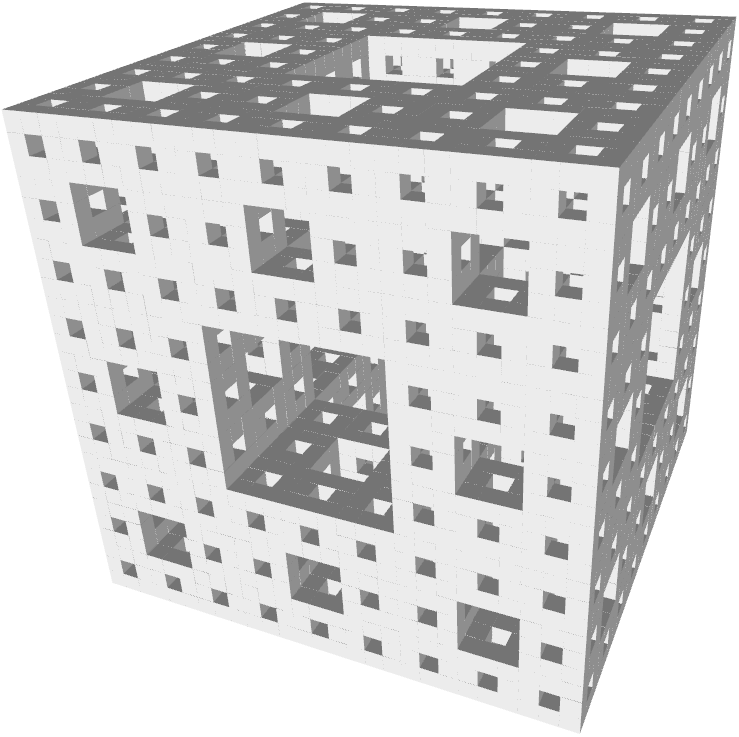
\includegraphics[width=\linewidth]{MengerSponge}
	\caption{Menger sponge created by \lsystem}
	\label{fig:introMengerSponge}
\end{wrapfigure}

The user interface will be web site which offers great accessibility.
Anybody around the world can use it from any device connected to the Internet like computers, laptops, tablets or smart phones.
Interface should be friendly to new users and also offer advanced features for experienced users.
Primary output format of the web based \lsystem processor will be 2D images but it will also be possible to create and display 3D outputs using modern HTML5 WebGL\footnote{
	WebGL (Web-based Graphics Library) is a cross-platform, royalty-free web standard for a low-level 3D graphics API based on OpenGL ES 2.0, exposed through the HTML5 Canvas element as Document Object Model interfaces.
	WebGL code executes on a computer display card's GPU (graphics processing unit).} technology directly in browser.
In \autoref{fig:introMengerSponge} is print-screen of Menger Sponge model displayed by WebGL.
Part of the web site will be gallery of \lsystems.
Any registered user can add his \lsystems to gallery along with some description and others can rate it.
This will help to create community of active users and it can also serve as learning tool for new users.
\nomenclature{HTML5}{hypertext markup language}
\nomenclature{WebGL}{web graphics library}
\nomenclature{API}{application programming interface}
\nomenclature{GPU}{graphics processing unit}

Second part of the application will be \lsystem processing library.
Although it will be designed to support demands of web interface, it will be independent and it should be usable in other applications.
During design of the library great emphasis will be placed on easy extensibility to make it as universal as possible.
It will be possible to extend the library by user.

New syntax for input will be designed to improve user experience especially for new users.
The syntax should be clean, easy to understand and remember.
%The syntax will cover all needs of library from defining \lsystems to configuring whole processing system.
%This will also ensure that whole input can be written in one file which will simplify source code sharing and saving.
%Parser generator will be used for creating robust and extensible parser.


\section*{Structure of the thesis}

In the first chapter are formal definition of \lsystems and their rewriting and interpretation principles.
Follows the description of \lsystem types and their properties.
At the end of the first chapter is a list of related \lsystem generators.

The second chapter is devoted to the design of the solution.
There is described how \lsystem processing library and web user interface works without implementation details.

Implementation detail of the project are discussed in the third chapter.
Sections in this chapters explains individual problems and their solutions.
The text accompanies actual source code snippets and diagrams for better explanation.

The fourth chapter summarizes the results.
Part of this chapter is showcase of images of generated \lsystems.

All used source codes of \lsystems are in syntax designed as a part of this work.
Syntax reference can be found in attachment \ref{chap:syntax}.
It is possible to process all source code on the web.
More information about figures in this thesis together with additional information and their source codes is in attachment \ref{chap:aboutFigures}.


































\chapter{\lsystems}

Brief history of \lsystems was mentioned in the introduction.
In this chapter we will describe \lsystems formally and we will explain rewriting and interpretation principles of \lsystems.
Main focus of this chapter is to describe \lsystem types.
At the end of the chapter is a list of related applications.



\section{Formal definition of \lsystem}

\lsystem $L$ is formally triplet $L = (\Sigma, \omega, R)$, where

\begin{itemize*}
	\item $\Sigma$ is \emph{alphabet}, non-empty set of symbols, $\Sigma^{*}$ is set of all words\footnote{Word is a sequence of symbols.} which can be created from the alphabet $\Sigma$, $\Sigma^{+}$ is set of all non-empty words which can be created from the the alphabet $\Sigma$,
	\item $\omega \in \Sigma^{+}$ is \emph{axiom} (also called seed), word defining the initial state of the \lsystem,
	\item $R \subset \Sigma \times \Sigma^{*}$ is a finite set of \emph{rewrite rules} (production rules), a rewrite rule defining rewriting symbol $s \in \Sigma$ to word $w \in \Sigma^{*}$ is written as $s \rightarrow w$.
\end{itemize*}

For any symbol $s \in \Sigma$ which does not appear on the left hand side of any rewrite rule in $R$, the identity rewrite rule $s \rightarrow s$ is assumed.
These symbols are called constants or terminals.

The formal definition of \lsystem is similar to deterministic context-free grammar but there are a few differences.
In such grammar we distinguish terminal and non-terminal symbols, but in \lsystems we do not define them explicitly (we define the identity rewrite rule for terminal symbols in \lsystems).
Next difference is in the initial string.
In the grammar is only one symbol as initial state but \lsystem allows a non-empty word.
The biggest difference is in rewriting principles which is described in following section.


\subsection{Rewriting principles of \lsystem}

Starting with axiom (0th iteration) in each iteration \emph{all} symbols are rewritten with rewrite rules forming next iteration.
All symbols can be rewritten because every symbol is on the left side of some rewrite rule.
% (if symbol have not been on the left side of some rewrite rule, identity rule would be defined).
There is only one way how to rewrite symbols in iteration thus rewriting is deterministic.
The result depends only on axiom.

Rewriting of symbols is parallel (all symbols are rewritten at once).
This means that when some symbol is rewritten, resulting symbols are not rewritten again in the same iteration.

Described rewriting principles distinguish an \lsystem and a formal grammar.
In the grammar there is not mandatory to rewrite all possible symbols (derivation of start state can result in more different derivations).
Thus, \lsystems are strict subset of languages.

\lsystem in \autoref{lsys:rrExample} produces strings shown in \autoref{fig:rrExampleResult}.
\lsystem starts with an axiom $A$ and two rewrite rules $A \rightarrow B$ and $B \rightarrow A, B$.
In the first iteration the axiom $A$ is rewritten by the first rewrite rule to $B$.
In the second iteration is $B$ rewritten with the second rewrite rule to symbols $A, B$.
In the third iteration is the first symbol $A$ rewritten to $B$ and the second symbol $B$ rewritten to $A, B$ which gives string $B, A, B$ and so on.

\begin{Lsystem}[label=lsys:rrExample,caption={Simple \lsystem as an example of rewriting principles}]
lsystem RewritingExample {
	set symbols axiom = A;
	set iterations = 6;
	set interpretEveryIteration = true;
	@rewrite A to B;@
	@rewrite B to A B;@
}
process all with SymbolPrinter;
\end{Lsystem}

\begin{table}[h]
	\centering
	\begin{tabular}{c l}
   		\toprule
   		Iteration & String of symbols \\
   		\midrule
		0 & A \\
		1 & B \\
		2 & A B \\
		3 & B A B \\
		4 & A B B A B \\
		5 & B A B A B B A B \\
		6 & A B B A B B A B A B B A B \\
		\bottomrule
	\end{tabular}
	\caption{Result of \lsystem in \autoref{lsys:rrExample}}
	\label{fig:rrExampleResult}
\end{table}


\subsection{Interpretation of \lsystem symbols}

Result of \lsystem rewriting is a string of symbols.
As it was mentioned in the \nameref{sec:Introduction} we can interpret string of symbols in any way for example as computer graphics or music.

The simplest and most common interpretation of \lsystem symbols is interpret them as 2D graphics elements like lines or polygons.
This interpretation is often called \emph{turtle graphics} and it will be used to interpret the most of \lsystems in this thesis.
This approach can be easily extended into 3D.

Let symbol $F$ is interpreted as \emph{draw line forward}, $+$ as \emph{turn left} and $-$ as turn right.
\autoref{fig:intSequences} shows interpreted strings of symbols using turtle graphics.
Initial direction is to the right.

\begin{figure}[h]
	\centering
	\subfloat[$F + F - - F + F$, turning angle: $60^{\circ}$]{
		
\includegraphics[scale=1]{IntTriangle}
	} ~
	\subfloat[$F + F - F - F + F$, turning angle: $90^{\circ}$]{
		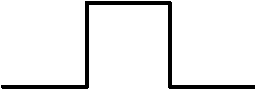
\includegraphics[scale=1]{IntSquare}
	} ~
	\subfloat[$F + F + + F - F - - F F - F$, turning angle: $60^{\circ}$]{
		\hspace{9mm}
\includegraphics[scale=1]{IntHexa}\hspace{9mm}
	}
	\caption{Examples of interpretation simple string of symbols}
	\label{fig:intSequences}
\end{figure}


More complex string of symbols as an example of interpretation is generated by \lsystem in \autoref{lsys:intExampleCode} where symbol $F$ is interpreted as \emph{draw line forward},
	symbol $+$ is interpreted as \emph{turn left} by 85 degrees and symbol $-$ as \emph{turn right} by 85 degrees (equally as \emph{turn left} by $-85$ degrees).
Result of interpretation of the first, second and fourth iteration is in \autoref{fig:intExample}.

\begin{Lsystem}[label=lsys:intExampleCode,caption={Symbol interpretation example}]
lsystem InterpretationExample {
	set symbols axiom = F;
	set iterations = 4;
	@interpret F as DrawForward(10);@
	@interpret + as TurnLeft(85);@
	@interpret - as TurnLeft(-85);@
	rewrite F to F + F - - F + F;
}
process all with SvgRenderer;
\end{Lsystem}

\begin{figure}[h]
	\subfloat{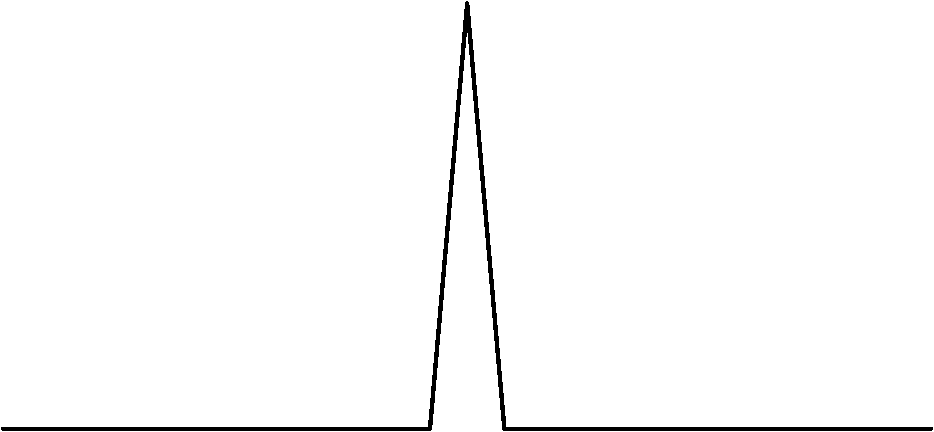
\includegraphics[scale=0.5]{Interpretation1}} \hfill
	\subfloat{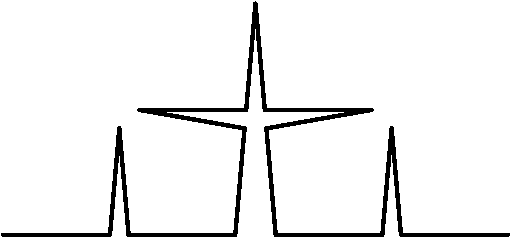
\includegraphics[scale=0.5]{Interpretation2}} \hfill
	\subfloat{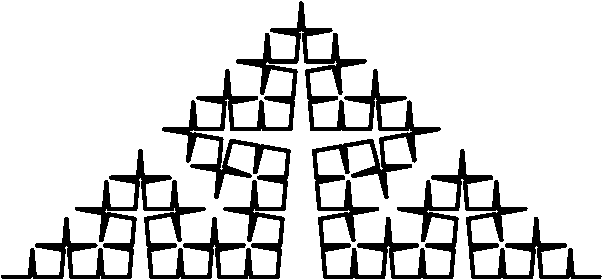
\includegraphics[scale=0.5]{Interpretation4}}
	\caption{The first, second and fourth iteration of the Cesaro curve (\autoref{lsys:intExampleCode})}
	\label{fig:intExample}
\end{figure}

\begin{figure}[h]
	
\includegraphics[width=1\linewidth]{RowOfTrees}
	\caption{Enhanced Cesaro curve from \autoref{fig:intExample} \cite[p.~48]{PL91}}
	\label{fig:rowOfTrees}
\end{figure}




































\clearpage

\section{\lsystem types}
\label{sec:lsysTypes}

In this section is described different types of \lsystems.
Some types may require an extension to the described formal definition of an \lsystem but this will be omitted here.

The \lsystems described so far are called \emph{deterministic \lsystems} because their rewriting system is deterministic.
\emph{Bracketed \lsystems} allow to save and load a state of the interpretation;
	this can be used to model branches of plants more easily.
\emph{Stochastic \lsystems} can randomize a result model to suppress its artificiality.
\emph{Context-sensitive \lsystems} allow to rewrite symbols depending on their context (the neighboring symbols around them).
Symbols in \emph{parametric \lsystems} can hold any number of arguments that can be used while rewriting or interpreting symbols.

Any of the above-described types can be combined together.



\subsection{Deterministic \lsystems}

\newcommand{\dzerolsystem}{\mbox{D0L-system}\xspace}
\newcommand{\dlsystem}{\mbox{dL-system}\xspace}


\begin{wrapfigure}{r}{0.50\textwidth}
	\vspace{-30pt}
	
\includegraphics[width=\linewidth]{BasicLsystem}
	\caption{Dragon curve}
	\label{fig:basicLsystem}
\end{wrapfigure}


The basic \lsystem type described by the previous formal definition is called a \dzerolsystem\footnote{A \dzerolsystem is also just called a \dlsystem~\cite{Zar04}.}.
\emph{D} means that the rewriting is deterministic and \emph{0} means it is context-free.
The result of a \dzerolsystem depends only on the initial string of symbols.

This type of \lsystem is often used to generate fractal curves.
With the \dzerolsystem in \autoref{fig:basicLsystem} we can generate the Dragon curve that you can see in \autoref{lsys:basicLsystemSrc}.

\begin{Lsystem}[label=lsys:basicLsystemSrc,caption={\dzerolsystem for the generation of the Dragon curve (\autoref{fig:basicLsystem})}]
lsystem DragonCurve {
	set iterations = 12;
	set symbols axiom = L;
	interpret R L as DrawForward(5);
	interpret + as TurnLeft(90);
	interpret - as TurnLeft(-90);
	rewrite L to L + R +;
	rewrite R to - L - R;
}
process all with SvgRenderer;
\end{Lsystem}


\subsection{Bracketed \lsystems}

A bracketed \lsystems\cite[p.~24]{PL91} extends basic \dzerolsystem with a branching system.
Branching is such a fundamental feature that Bracketed \lsystems are often just called \lsystems.

A branching system brings two new commands to the symbol interpretation system: \emph{start branch} and \emph{end branch}.
These commands are nearly always represented as bracket symbols (from which bracketed \lsystems got their name).
An open bracket "\texttt{[}" as a start branch and close bracket "\texttt{]}" as a close branch.

The start branch command saves the state of interpretation, which can then be loaded by end the branch command later.
In turtle graphics, the interpretation state is the position, orientation and drawing color of the turtle.
More than one state can be saved at the same time, and the last saved state will be loaded first.
This behavior seems natural and could be compared to a pairing of brackets.

Branching extends a linear string of symbols to a tree structure.
Individual branches do not affect each other nor their root.
This allows plants to be modeled more easily and to create more complex models.

The bracketed \lsystem in \autoref{lsys:branchingSrc} demonstrates a use of the branching system to produce a plant-like model as can be seen in \autoref{fig:branching}.
Note that the color of segments indicates their type and age.
Black segments are drawn with the symbol \texttt{F} and they represent segments from the previous iteration.
Green segments are drawn with the symbol \texttt{A} and they are new compared to the previous iteration.

\begin{Lsystem}[label=lsys:branchingSrc,caption={A bracketed \lsystem that which creates a plant-like model (\autoref{fig:branching})}]
lsystem PythagorasTree {
	set symbols axiom = A;
	set initialAngle = 90;
	set iterations = 4;	
	interpret A F as DrawForward(16);
	interpret + as TurnLeft(45);
	interpret - as TurnLeft(-45);
	@interpret [ as StartBranch;@
	@interpret ] as EndBranch;@
	rewrite A to F [ + A ] [ - A ] F A;
	rewrite F to F F;
}
process all with SvgRenderer;
\end{Lsystem}

\begin{figure}[h]
	\centering
	\subfloat{
\includegraphics[scale=1]{Branching1}} ~
	\subfloat{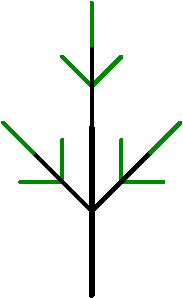
\includegraphics[scale=1]{Branching2}} ~
	\subfloat{
\includegraphics[scale=1]{Branching3}} ~
	\subfloat{
\includegraphics[scale=1]{Branching4}}
	\caption[The first four iterations of a bracketed \lsystem]{The first four iterations of the bracketed \lsystem in \autoref{lsys:branchingSrc}}
	\label{fig:branching}
\end{figure}



\subsection{Stochastic \lsystems}

\newcommand{\zerolsystem}{\mbox{0L-system}\xspace}
\newcommand{\zerolsystems}{\mbox{0L-systems}\xspace}

All plant models generated by the same deterministic \lsystem are identical.
However, a forest made by trees which are all identical looks artificial and can not be used in films or video games.
Stochastic \lsystems solve this problem because they can produce a randomized model.
Stochastic \lsystems are called \zerolsystem where 0 means they are context-free.

Randomization of a model produced by stochastic a \lsystem can be done in two places, in the rewrite rules or in the interpretation of symbols (or in both).
Randomization in interpretation can only change the properties of such interpreted symbols as lengths of lines or turning angles, while the topology of the model remains unchanged.
This is in contrast to rewrite rule randomization that can also change the topology of a model.
Rewrite rule randomization is achieved by defining more replacements for one rewrite rule.
The rewriting system will pick a random replacement if the rewrite rule is applied.
Each replacement can have a different probability of being picked.

In \autoref{fig:randComparison}, three models of a plant generated by stochastic \lsystems are shown.
The first image (\ref{fig:randComparisonNo}) was generated without any randomization.
The second image (\ref{fig:randComparisonInt}) was generated with interpretation randomization of line lengths and angles.
For the last image (\ref{fig:randComparisonBoth}) was used the rewrite rule randomization which changed the topology of the model (\autoref{lsys:randExample}).

\begin{figure}[h]
	\centering
	\subfloat[No randomization]{
		\label{fig:randComparisonNo}
		
\includegraphics[width=0.3\textwidth]{StochasticLsystemExample-NoStochasism}
	} ~
	\subfloat[Angles, lengths randomized]{
		\label{fig:randComparisonInt}
		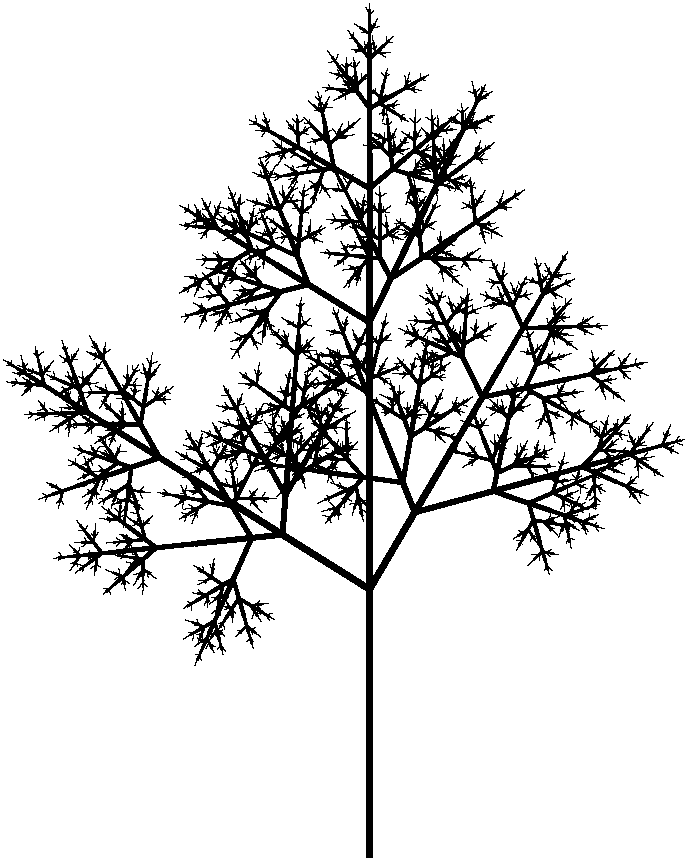
\includegraphics[width=0.32\textwidth]{StochasticLsystemExample-InterpretationStochasism}
	} ~
	\subfloat[Also topology randomized]{
		~
		\label{fig:randComparisonBoth}
		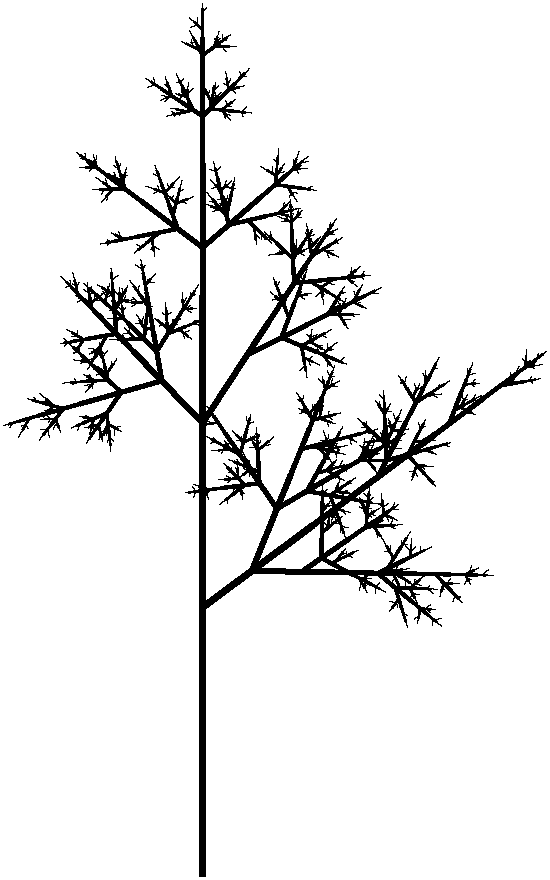
\includegraphics[width=0.25\textwidth]{StochasticLsystemExample-BothStochasism}
		~
	}
	\caption{A comparison between a non-randomized and randomized plant model}
	\label{fig:randComparison}
\end{figure}

\begin{Lsystem}[label=lsys:randExample,caption={Stochastic \lsystem with randomized interpretation of symbols and rewrite rule replacements}]
lsystem StochasticLsystemExample {
	set symbols axiom = X;
	set iterations = 8;
	set initialAngle = 90;
	interpret F(age) as DrawForward(@1.8^age*random(0.5,1.5)@, age/2);
	interpret + as TurnLeft(@45 + random(-20, 20)@);
	interpret - as TurnLeft(@-45 + random(-20, 20)@);
	interpret [ as StartBranch;
	interpret ] as EndBranch;
	rewrite F(age) to F(age + 1);
	@rewrite X@
		@to F(1) [ + X ] [ - X ] F(1) X  weight 4 or@
		@to F(1) [ + X ]         F(1) X  weight 1 or@
		@to F(1)         [ - X ] F(1) X  weight 1;@
}
process all with SvgRenderer;
\end{Lsystem}


\subsection{Context-sensitive \lsystems}

\newcommand{\onelsystems}{\mbox{1L-systems}\xspace}
\newcommand{\twolsystems}{\mbox{2L-systems}\xspace}

The rewriting of symbols in \zerolsystems is context-free; the rewrite rules are applied to the symbols regardless of their context (the symbols around them).
However, the rewriting of a symbol can also depend on its context.
This is useful in simulating the flow of signals (nutrients or hormones) in a plant model that, for example, attempts to demonstrate natural plant growth~\citep{PL91}.

Formally there are two types of context-sensitive L-systems, \onelsystems and \twolsystems.
The rewrite rules of \onelsystems checks the context only to one side (left or right), whereas the rewrite rules of \twolsystems checks the context on both sides.
Since \onelsystems are just \twolsystems with one context empty we will consider context-sensitive \lsystems as \twolsystems.

The context-sensitive \lsystem in \autoref{lsys:signalPropagarionSrc} shows a simulation of signal propagation in a string of symbols; the result is given in \autoref{fig:signalPropagarion}.

\begin{Lsystem}[label=lsys:signalPropagarionSrc,caption={Context-sensitive \lsystem simulating signal propagation}]
lsystem RewritingExample {
	set symbols axiom = B A A A A A;
	set iterations = 6;
	set interpretEveryIteration = true;
	@rewrite {B} A     to B;@
	@rewrite     B {A} to A;@
}
process all with SymbolPrinter;
\end{Lsystem}

\begin{table}[h]
	\centering
	\begin{tabular}{c l}
   		\toprule
   		Iteration & String of symbols \\
   		\midrule
		0 & B A A A A A \\
		1 & A B A A A A \\
		2 & A A B A A A \\
		3 & A A A B A A \\
		4 & A A A A B A \\
		5 & A A A A A B \\
		6 & A A A A A A \\
		\bottomrule
	\end{tabular}
	\caption{An axiom and the first 6 iterations of an \lsystem in \autoref{lsys:signalPropagarionSrc} showing signal propagation in the given string of symbols}
	\label{fig:signalPropagarion}
\end{table}


\subsubsection{Context-sensitive bracketed \lsystems}
\label{sec:bracketedLsystems}

If we add context-sensitive rewrite rules to bracketed \lsystems the situation becomes more difficult.
The context-matching procedure must take into account the branches.
The following rules define the natural behavior of context between branches:
\begin{enumerate*}
	\item \label{enum:ctxRule1} two symbols are neighbors even if there are some branches between them,
	\item \label{enum:ctxRule2} the left neighbor of the first symbol in a branch is a symbol before the branch,
	\item \label{enum:ctxRule3} the last symbol in a branch does not have a right neighbor,
	\item \label{enum:ctxRule4} unmatched symbols at the end of a branch are ignored,
	\item \label{enum:ctxRule5} the order of branches is insignificant.
\end{enumerate*}

In \autoref{tbl:bracketCtxt} is a few examples of how a symbol with its context will match (or not) a given string of symbols with respect to the context-matching rules mentioned above.
\begin{table}[h]
	\centering
	\begin{tabular}{c c c | p{128pt} c c}
   		\toprule
   		Left ctx. & Symbol & Right ctx. & Symbol string & Match & Rule\\
   		\midrule
		 & X & Y & A B {\btHL\bf X} [ A [ B ] ] [ C ] {\btHL\bf Y} & yes & \ref{enum:ctxRule1} \\
		 & X & Y & A B X [ Y B ] C Y & no &  \\
		 Y & X & & A B {\btHL\bf Y [ X} A B ] C & yes & \ref{enum:ctxRule2} \\
		 Y & X & & A B {\btHL\bf Y [ [ X} A ] B ] C & yes & \ref{enum:ctxRule2} \\
		 & X & Y & A [ B X ] Y & no & \ref{enum:ctxRule3} \\
		 & X & [ Y ] & A B {\btHL\bf X [ Y} A B ] A  & yes & \ref{enum:ctxRule4} \\
		 & X & [ [ Y ] ] & A B {\btHL\bf X [ [ Y} A B ] C ] & yes & \ref{enum:ctxRule4} \\
		 & X & [ Y ] & A B {\btHL\bf X} [ A B ] {\btHL\bf{}[ Y} ] A  & yes & \ref{enum:ctxRule5} \\
		 & X & [ Y ] [ Z ] & A B {\btHL\bf X [ Z} ] {\btHL\bf{}[ Y} ] A  & yes & \ref{enum:ctxRule5} \\
		\bottomrule
	\end{tabular}
	\caption{Examples of context matching in bracketed \lsystems}
	\label{tbl:bracketCtxt}
\end{table}

Context in bracketed \lsystems can be used for the propagation of signals through tree structures.
There are two basic types of signals: the first is the \emph{acropetal} signal which spreads from the root to branches; and the second signal is \emph{basipetal} which spreads in the opposite way i.e. from branches to root.
This can be very useful in plant modeling.

\autoref{fig:signalPropagation} shows a simulation of acropetal (\ref{fig:acropetalSignal}) and basipetal (\ref{fig:basipetalSignal}) signals in a static plant-like structure.
Each figure shows the first 5 iterations and segments with the signal marked as a bolder line.
The \lsystem in \autoref{lsys:signalPropagation} simulates acropetal signal propagation and its result is in \autoref{fig:acropetalSignal} (image) and \autoref{fig:signalPropagationTable} (symbols).

\begin{figure}[h!]
	\centering
	\subfloat[Acropetal signal propagation]{
		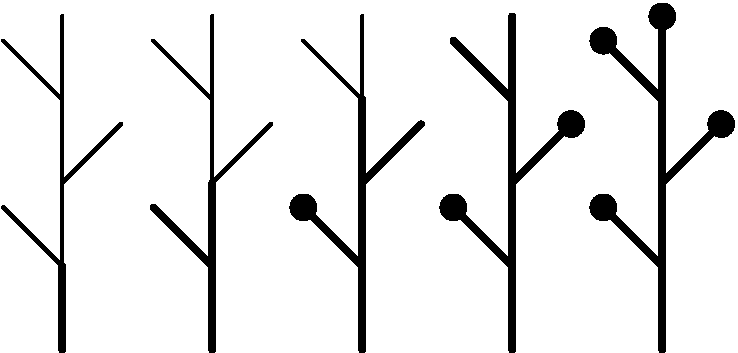
\includegraphics[scale=0.55]{AcropetalSignal}
		\label{fig:acropetalSignal}
	}
	\hspace{2mm}
	\subfloat[Basipetal signal propagation]{
		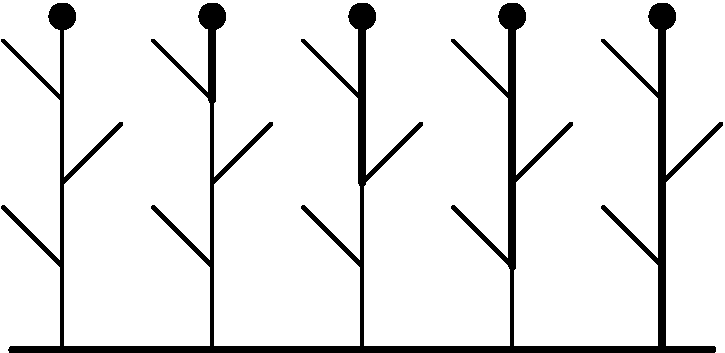
\includegraphics[scale=0.55]{BasipetalSignal}
		\label{fig:basipetalSignal}
	}
	\caption{Signal propagation simulated with context-sensitive bracketed \lsystems}
	\label{fig:signalPropagation}
\end{figure}

\begin{Lsystem}[label=lsys:signalPropagation,caption={The \lsystem simulating acropetal signal propagation (\autoref{fig:acropetalSignal})}]
lsystem AcropetalSignal extends Branches {
	set symbols axiom = B [ + A ] A [ - A ] A [ + A ] A;
	// ignore + and - symbols in context search
	@set symbols contextIgnore = + -;@
	set iterations = 3;
	// interpret every iteration to see signal propagation
	set interpretEveryIteration = true;
	set initialAngle = 90;
	interpret A as DrawForward(50, 2);
	interpret B as DrawForward(50, 4);
	interpret + as TurnLeft(45);
	interpret - as TurnLeft(-45);
	@rewrite { B } A to B;@
}
process all with SvgRenderer;
\end{Lsystem}


\begin{table}[h]
	\centering
	\begin{tabular}{c c}
   		\toprule
   		Iteration & String of symbols \\
   		\midrule
		0 & B [ + A ] A [ - A ] A [ + A ] A \\
		1 & B [ + B ] B [ - A ] A [ + A ] A \\
		2 & B [ + B ] B [ - B ] B [ + A ] A \\
		3 & B [ + B ] B [ - B ] B [ + B ] B \\
		\bottomrule
	\end{tabular}
	\caption{The result of the \lsystem simulating acropetal signal propagation in \autoref{lsys:signalPropagation}}
	\label{fig:signalPropagationTable}
\end{table}


\subsection{Parametric \lsystems}

Symbols in parametric \lsystems can hold any number of arguments.
Arguments are often floating point numbers, but they can be much more complicated structures.
Arguments can be used in interpretation definition to send values like color or length of line to an interpretation routine.
Arguments can also be used in rewrite rules to determine whether to rewrite a symbol or not, and to determine new arguments for rewritten symbols.
In context \twolsystems it is also possible to get arguments from symbols in context and use them in rewrite rules.

The \lsystem in \autoref{fig:scParams} shows an example of how the parameters of symbols can be used in interpretation methods and in rewrite rules together with the result.

\newsavebox{\lstBox}
\begin{lrbox}{\lstBox}
\begin{Lsystem50}
lsystem Circles {
	set symbols axiom =	[ X ] +
		[ X ] + [ X ] + [ X ];
	set iterations = 7;
	interpret F as MoveForward;
	interpret K as DrawCircle;
	interpret + as @TurnLeft(90)@;
	interpret - as @TurnLeft(-90)@;
	interpret [ as StartBranch;
	interpret ] as EndBranch;
	rewrite @K(n) to K(2*n)@;
	rewrite @F(n) to F(2*n)@;
	rewrite X to @K(2) F(3)@
		[ + X ] [ - X ] X;
}
process all with SvgRenderer;
\end{Lsystem50}
\end{lrbox}

\begin{figure}[h!]
	\subfloat{
		\usebox{\lstBox}
	} \hfill
	\subfloat{
		\minipage{0.47\linewidth}\noindent
		
\includegraphics[width=\textwidth]{Circles}
		\endminipage
	}
	\caption{Parameters usage in \lsystem interpretation methods and in rewrite rules along with the result}
	\label{fig:scParams}
\end{figure}

In \autoref{fig:redEndPythagoras} is more complicated model, the Pythagoras tree.
Detailed instructions for its construction with \lsystems are described in appendix \ref{chap:userDoc}.

\begin{figure}[H]
	\centering
	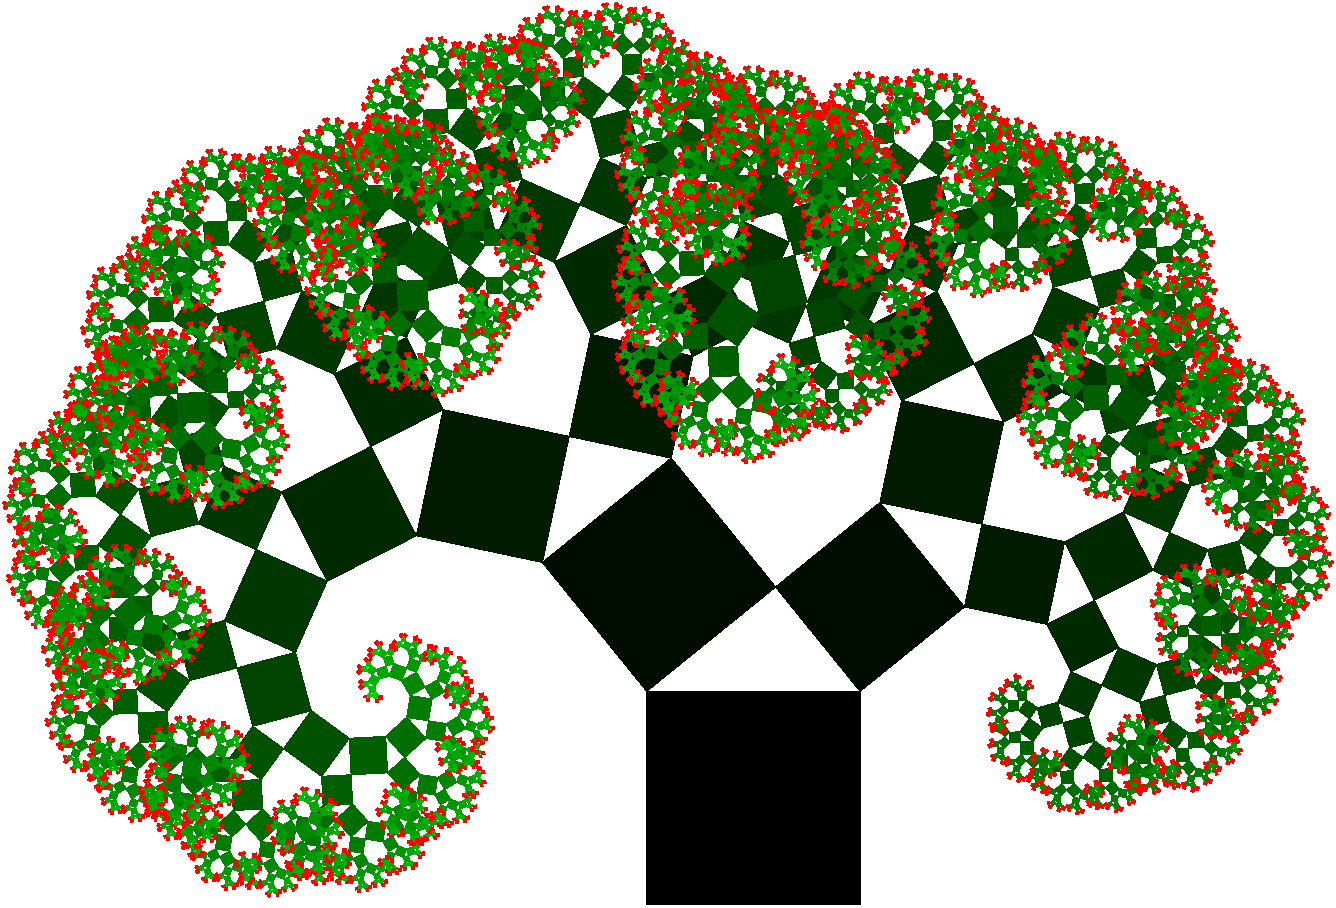
\includegraphics[width=\linewidth]{PythagorasTree2dRedEnd}
	\caption{Pythagoras tree created with parametric \lsystem}
	\label{fig:redEndPythagoras}
\end{figure}


































\clearpage

\section{Related \lsystem generators}

In this section are listed other computer programs or web pages that allow to process \lsystems and eventually interpret them in most cases as an image.

\subsection{Web based}
\label{sec:WebBasedGenerators}

\subsubsection{\lsystem generator by Michael Norris}
\srcurl{http://www.michaelnorris.info/software/l-system-generator.html}

\noindent
Simple script which allows to set basic properties of \lsystem namely number of iterations, axiom and up to 15 rewrite rules.
Result is a list of strings of symbols from all iterations (it does not interpret symbols).

This site can be used to familiarize with rewriting principles of \lsystems but it offers no additional functionality.


\subsubsection{Lindenmayer power by MadFlame Software}
\srcurl{http://madflame991.blogspot.com/p/lindenmayer-power.html}

\noindent
\lsystem generator which allows to set basic properties of \lsystem and interpretation for each symbol.
Symbols can be interpreted using turtle graphics or they can define or modify value of a variable.
All iterations are listed as text and drawn on screen as well.

Possibility to work with variables makes it relatively powerful system but it is possible to draw only with a thin black line.
Also the syntax is not very user-friendly and user the interface is hard to use (and the script it is not very stable).
The size of the output window is only $500 \times 500$ pixels and output can not be saved otherwise than using print-screen.


\subsubsection{\lsystem generator by Nolan Carroll}	
\srcurl{http://nolandc.com/sandbox/fractals/}

\noindent
\lsystem generator with a nice looking interface where it is possible to set basic properties of an \lsystem.
The interpretation of symbols is fixed.
Last iteration of \lsystem is drawn on the screen using animation (line by line from the starting position).

Interface is user friendly but only drawable interpretation of symbol is black line.
There is no help nor examples thus it is hard to use for inexperienced user.
Output is drawn on canvas which fills entire area of web browser but it can not be saved otherwise than using print-screen.


\subsubsection{VRML \lsystem generator by Patrick Murris}
\srcurl{http://www.alpix.com/vrml/lsys.htm}
  
\noindent
\lsystem generator which can generate 3D VRML model.
Basic properties of \lsystem and interpretation can be set and output can be produced into VRML 1.0, 2.0 or string.

The problem is that VRML plugin is needed for displaying 3D models.



\subsubsection{\lsystem generator by John Snyders}
\srcurl{http://hardlikesoftware.com/projects/lsystem/lsystem.html}

\noindent
At first sight it is sophisticated \lsystem generator which can rewrite symbols with parameters and do context-sensitive rewriting.
Result is drawn on a page as an animation of development and a progress bar shows its status.
The biggest drawback is that \lsystems are hard-coded in JavaScript and it is only possible to change the number of iterations.

This \lsystem generator contains many examples and output is rendered as image which can be saved but examples are the only thing what it can produce.


\subsubsection{WWW \lsystem Explorer by Zdík Kudrle}
\srcurl{http://zdeeck.borg.cz/wlse/l-system.php}

\begin{wrapfigure}{r}{0.45\textwidth}
	\vspace{-20pt}
	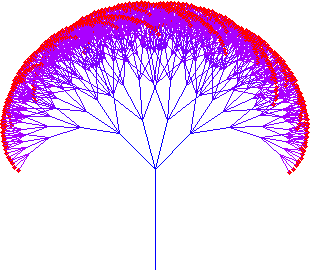
\includegraphics[width=\linewidth]{WwwLsystemExplorer}
	\caption{Image produced by WWW \lsystem Explorer}
	\label{fig:lsysExplorer}
\end{wrapfigure}

\noindent
\lsystem generator with well-arranged user interface where is possible to set basic properties of the generated \lsystems.
The interpretation of symbols is fixed and it uses unusual set of interpretation methods like \emph{pen up} and \emph{pen down} instead o traditional \emph{draw line} and \emph{move forward}.
The last iteration is drawn as an image by server-side PHP script thus output can be downloaded easily.
It is possible to set line color (even to color gradient) and background color of the image.
Size of the output image can be set freely.

This web-based generator is the best among the generators listed in this section.
It contains well written help section and a few examples.
However it can not do context rewriting and symbols can't hold any parameters.
The length of drawn lines or turns can be affected only by increasing \emph{depth level} and setting the change ratio.
Example of plantlike model produced by WWW \lsystem Explorer is in \autoref{fig:lsysExplorer}.




\subsection{Desktop applications}
\label{sec:DesktopGenerators}

\subsubsection{\lsystems explorer by James Matthews}
\label{sec:LsystemExplorer}
\srcurl{http://www.generation5.org/content/2002/lse.asp}

\noindent
Simple desktop application which renders \lsystems in the application window.
Basic properties of \lsystem and its interpretation can be edited in dialog window but interpretation for individual symbols can not be changed.
It is possible to move and zoom the model with a mouse.
\lsystems can be saved or loaded into text file and drawn image can be saved to clipboard.

\lsystems explorer can be used for generation of simple models but it is not possible to do context rewriting or use symbols parameters.
Even line thickness can not be changed.
User interface for editing \lsystem is very simple (it is possible to show rewrite rules only for one symbol at a time).


\subsubsection{\lsystem Vector Generator by Dmitry Malutin}
\srcurl{http://xaraxtv.at.tut.by/lsvg.htm}

\begin{wrapfigure}{r}{0.4\textwidth}
	\vspace{-20pt}
	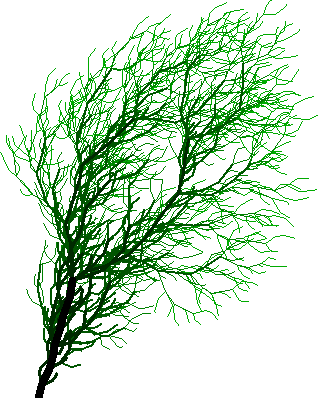
\includegraphics[width=\linewidth]{LsystemVectorGenerator}
	\caption{Plant example from \lsystem Vector Generator}
	\label{fig:lsvg}
\end{wrapfigure}

\noindent
Similar application to the \nameref{sec:LsystemExplorer} but with better user interface and it is also possible to randomize line lengths or turn angles.
Nice feature is the \emph{angle wizard} which displays grid of \lsystems each with different setting of turning angle and you can pick what you like. %!!!!!!!!!!!
Drawn lines can be automatically closed to form polygons.
It is possible to save image as AI (Adobe Illustrator) or WMF (Windows Metafile) file which are not very common formats.

Application contains hundreds of examples but it lacks any advanced types of \lsystems or interpretation settings.
Application window size is about $700 \times 550$ pixels and it can not be resided.
One of built-in examples with randomized angles and line lengths is in \autoref{fig:lsvg}.


\subsubsection{\lsystem 4 by Timothy Perz}
\srcurl{http://www.oocities.org/tperz/L4About.htm}

\noindent
\lsystem 4 is relatively advanced tool for generating models with \lsystems.
Besides all basic functionality it is possible to create 3D models with custom textures.
Models can be saved as raster images (BMP or JPEG) or they can be exported to AutoCAD DXF format.
Interpreting capabilities are quite good but it can do only deterministic rewriting with limited usage of parameters.

Table of symbols interpretations (which are not changeable) can be displayed at right side of application which is a nice feature.
\lsystem 4 has good capabilities in producing of 3D output but the input syntax is very compact and hard to read.
Also more advanced \lsystem types like context-sensitive or parametric \lsystems are not supported.

\newcommand{\lstudio}{\mbox{L-studio}\xspace}

\subsubsection{\lstudio by Przemysław Prusinkiewicz et. al}
\srcurl{http://algorithmicbotany.org/lstudio/}

\noindent
\lstudio is probably one of the best applications designed for modeling plants with \lsystems.
\lstudio is not a single program but it is complex solution that consists of many tools.
\lstudio can process all types of \lsystems described in \autoref{sec:lsysTypes} and also it can produce animation of plant growth.
With \lstudio is possible to model 3D models of plants with regards to environment like wind, gravity, the space around plant, sunlight, etc.
Output model can be saved in many formats like Wavefront OBJ, Postscript, BMP or it can be rendered with built in ray-tracer to produce photo-realistic images.

Even there is many examples of plant models and extensive help it is not easy to start using it.
The syntax is very compact and quite unclear for a new user.

Application is not free-ware but a demo version can be downloaded.
After evaluation period it is still possible to use it but it is not possible to export images and the previews have watermark.
In \autoref{fig:lstudio} is one of the most beautiful examples in \lstudio, the Lily.


\begin{figure}[h]
	\centering
	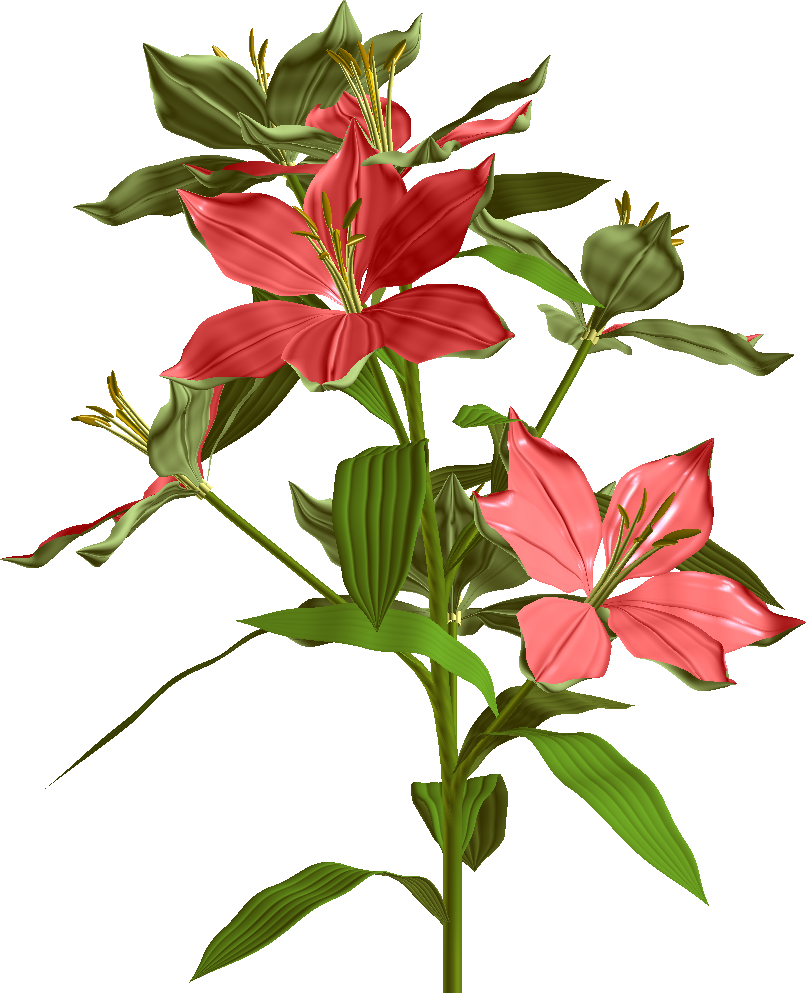
\includegraphics[width=0.8\linewidth]{Lily}
	\caption{Model of Lily produced by \lstudio}
	\label{fig:lstudio}
\end{figure}

























































\chapter{Design}

In this chapter is described design of solution and explained decisions that were made.
Implementation details are described in \autoref{chap:implementation}.

In the first section is described design of \lsystem processing library.
Library process input with component-based approach.
Core of the library is responsible for creating system of connected components (components graph) but processing of \lsystem itself is fully under control of components.
Components can be created by user which bring freedom to \lsystem processing.

Library it will contain predefined components to be possible to process \lsystems without need of creating custom components.
Design of these components is described in the second section.
These components will also serve as an example for users who want to implement their own processing system.

In the third section is described design of online web user interface.
It uses library and components to process input so it will also serve as an example of usage.




\section{\lsystem processing library design}

\lsystem processing library design will provide application interface (API) for processing of \lsystems.
The main feature will be extensibility....





















\clearpage

\section{Processing system}
\label{sec:design-components}

As discussed in the previous chapter, the processing system of the library relies on the components.
The core of the library is responsible for just creating the component graph.
The processing of an \lsystem and production of results is fully under the control of the component graph.
This gives absolute freedom to the user in implementing the process system.

However it is hard to design and implement the whole \lsystem processing system from scratch.
The library contains a rich set of predefined components from which can be assembled many different component graphs.
The predefined components have a general interface which allows the user to reuse or extend them in order to add new functionality with a minimum of effort.


\subsection{Basic component system}

The component system designed in this section is primarily used for processing \lsystems to produce 2D and 3D graphics in the web interface.
However, the component system is designed to be extensible to any output type.

\lsystems are generally processed in two phases.
The first phase is rewriting where the axiom (the initial string of symbols) is rewritten by the rewrite rules, and the second phase is interpreting the resulting string of symbols.
This can be done with two components, the Rewriter -- which is responsible for rewriting the \lsystem to a given iteration -- and the Interpreter -- which is responsible for interpreting symbols and producing output (Fig. \ref{fig:simpleSystem}).

\begin{figure}[h!]
	\centering
	\begin{tikzpicture}[->,auto,node distance=3cm,>=latex,shorten >=2pt]
		\node (in) [coord] {};
		\node (rw) [block, right of=in] {Rewriter};
		\node (int) [block, right=1cm of rw] {Interpreter};
		\node (out) [coord, right of=int] {};
		
		\draw (in) -- node {input} (rw);
		\draw (rw) -- (int);
		\draw (int) -- node {output} (out);
	\end{tikzpicture}
	\caption{Simple \lsystem processing system}
	\label{fig:simpleSystem}
\end{figure}

However the components in the system in \autoref{fig:simpleSystem} have too many tasks to do, and thus they will be complicated to implement and hard to extend and test.

The system in \autoref{fig:advancedSystem} was created by a subdivision of the previous system.
The Rewriter component was split to the Rewriter and the Iterator.
The (new) Rewriter will just do the rewriting of some given symbols and the Iterator will control the iterating of the \lsystem (repetitive rewriting).
The Interpreter component was split to the Interpreter and the Renderer.
The (new) Interpreter will handle the interpreting of symbols: which means keep position of the virtual "turtle" in space, saving and loading of states, etc.
The Renderer will just produce the output.
If we need to create a different output type we only have to implement the new renderer component and the rest of the system will remain unchanged.

\begin{figure}[h!]
	\centering
	\begin{tikzpicture}[->,auto,node distance=3cm,>=latex,shorten >=2pt]
		\node (rw) [block] {Rewriter};
		\node (iter) [block, right of=rw] {Iterator};
		\node (in) [coord, above of=iter, node distance=15mm] {};
		\node (inter) [block, right of=iter] {Interpreter};
		\node (rend) [block, right of=inter] {Renderer};
		\node (out) [coord, right of=rend] {};
		
		\draw (rw) to[bend left=40] (iter);
		\draw (iter) to[bend left=40] (rw);
		\draw (in) -- node {input} (iter);
		\draw (iter) -- (inter);
		\draw (inter) -- (rend);
		\draw (rend) -- node {output} (out);
	\end{tikzpicture}
	\caption{Subdivided \lsystem processing system}
	\label{fig:advancedSystem}
\end{figure}


\subsection{Component system extensions}
\label{sec:caller}

The system in \autoref{fig:callerComponent} can be enhanced even more.
Every component that interprets \lsystem symbols needs to translate symbols to interpretation methods.
The translation can be implemented by every component individually.
However, the translation can be done by a specialized component called the \emph{Interpreter caller}.
This component can be smart enough to explore all the components in the system, find all the interpretation methods of all components and do translation automatically.
This causes an automatic "connection" of all interpreters to the interpreter caller.

More interpreters can be used to advantage: for example, for processing \lsystems which interact with themselves or their Environment \cite{MP96}.
One interpreter actually creates the result model and the second interpreter simulates the environment.

\begin{figure}[h!]
	\centering
	\begin{tikzpicture}[->,auto,node distance=3cm,>=latex,shorten >=2pt]
		\node (iter) [block] {Iterator};
		\node (in) [coord, above of=iter, node distance=15mm] {};
		\node (rw) [block, below of=iter, node distance=20mm] {Rewriter};
		\node (caller) [blockx, right of=iter, node distance=35mm] {Interpreter caller};
		\node (inter) [block, right of=caller, node distance=40mm] {Interpreter};
		\node (env) [block, below of=inter, node distance=20mm] {Environment module};
		\node (rend) [block, right of=inter] {Renderer};
		\node (out) [coord, right of=rend] {};
		
		\draw (rw) to[bend left=40] (iter);
		\draw (iter) to[bend left=40] (rw);
		\draw (in) -- node {input} (iter);
		\draw (iter) -- (caller);
		\draw [dashed] (caller) -- (inter);
		\draw [dashed] (caller) -- (env);
		\draw (inter) -- (rend);
		\draw (env) -- (rw);
		\draw (rend) -- node {output} (out);
	\end{tikzpicture}
	\caption[Automated interpreter caller]{The Interpreter caller which automatically calls interpretation methods of any components}
	\label{fig:callerComponent}
\end{figure}




The next necessary component is called the \emph{Random provider}.
It provides controlled behavior for random number generation as described in \autoref{sec:measuring}.
This component provides a function which returns a random number and it can be called by other components or by the user in the \lsystem definition.
This component is connected to the iterator to correctly the reset random seed at every pass.

The \emph{axiom provider} is the next extending component and it provides the axiom to the Iterator.
The axiom provider is only a "wrapper" around a single symbol property called the axiom.
The Iterator is designed generally to take the axiom from any component implementing \emph{ISymbolProvider} interface so it is possible to connect, for example, another rewriter as the axiom provider (Fig. \ref{fig:inputProvider}).

\begin{figure}[h!]
	\centering
	\begin{tikzpicture}[->,auto,node distance=3cm,>=latex,shorten >=2pt]
		\node (iter) [block] {Iterator};
		\node (rw) [block, left of=iter] {Main rewriter};
		\node (rw2) [blockx, above of=iter, node distance=20mm] {Input rewriter};
		\node (in) [coord, above of=rw2, node distance=15mm] {};
		\node (caller) [block, right of=iter, node distance=35mm] {Interpreter caller};
		\node (inter) [block, above of=caller, node distance=20mm] {Interpreter};
		\node (rend) [block, right of=inter] {Renderer};
		\node (out) [coord, right of=rend] {};
		
		\draw (rw) to[bend left=40] (iter);
		\draw (iter) to[bend left=40] (rw);
		\draw (rw2) -- (iter);
		\draw (in) -- node {input} (rw2);
		\draw (iter) -- (caller);
		\draw [dashed] (caller) -- (inter);
		\draw (inter) -- (rend);
		\draw (rend) -- node {output} (out);
	\end{tikzpicture}
	\caption{Input for the iterator can be supplied by another component}
	\label{fig:inputProvider}
\end{figure}



\subsection{Interpretation of a symbol as another \lsystem}
\label{sec:innerLsystem}

In some situations it can be handy to interpret a symbol as another \lsystem.
The component system of the library is very versatile and it allows the creation of a specialized component which will be responsible for just this feature.

The component is called the \emph{Inner \lsystem processor}.
It is connected to the Interpreter caller and when the caller needs to interpret a symbol as an \lsystem it will call the Inner \lsystem processor to take care of this.
A component graph with the Inner \lsystem processor component is shown in \autoref{fig:innerSystem}.

The Inner \lsystem processor works internally in a similar way to that of the Process manager (see \autoref{sec:inputProcessing}).
For every processed symbol it builds a new components graph for processing the inner \lsystem.
The components graph can be specified by a special process configuration which needs to be defined in the input%
	\footnote{
		The only implementation of the Inner \lsystem processor the \hyperref[Malsys.Processing.Components.Common.LsystemInLsystemProcessor]{\emph{LsystemInLsystemProcessor}} component uses the process configuration called \emph{InnerLsystemConfig} for creating the inner component graph.
		This process configuration must be defined (see the definition in the Standard library \ref{sec:innerLsystemConfig}).}.
The interpreter caller in the inner component graph is automatically connected to all interpreters in the original component graph (see \autoref{sec:caller}), therefore the inner \lsystem is interpreted by the same interpreter as the main \lsystem.
The inner interpreter caller is also connected to the Inner \lsystem processor: thus it is possible to interpret a symbol as another \lsystem even in the inner \lsystem.

The creation of the inner component graph is a relatively complex operation.
The created and used component graphs are cached and reused later which improves the performance.

\begin{figure}[h!]
	\centering
	\begin{tikzpicture}[->,auto,node distance=3cm,>=latex,shorten >=2pt]
		\node (it) [block] {Iterator};
		\node (in) [coord, above of=it, node distance=15mm] {};
		\node (rw) [block, left of=it] {Rewriter};
		\node (caller) [block, right of=it, node distance=35mm] {Interpreter caller};
		\node (inter) [block, above of=caller, node distance=20mm] {Interpreter};
		\node (rend) [block, right of=inter] {Renderer};
		\node (out) [coord, right of=rend] {};
		\node (inner) [blockx, below of=caller, node distance=20mm] {Inner L-system processor};
		\node (innerIt) [blockx, below of=inner, node distance=22mm] {Inner iterator};
		\node (innerRw) [blockx, left of=innerIt, node distance=33mm] {Inner rewriter};
		\node (innerCaller) [blockx, right of=innerIt, node distance=32mm] {Inner caller};
		
		\node (innerArea) [area,fit=(innerIt) (innerRw) (innerCaller), label=above left:Inner component graph] {};
		
		\draw (rw) to[bend left=40] (it);
		\draw (it) to[bend left=40] (rw);
		\draw (in) -- node {input} (it);
		\draw (it) -- (caller);
		\draw (caller) -- (inner);
		\draw [dashed] (caller) -- (inter);
		\draw (inter) -- (rend);
		\draw (rend) -- node {output} (out);
		
		\draw [snakeline] (inner) -- (innerArea);
		\draw (innerRw) to[bend left=20] (innerIt);
		\draw (innerIt) to[bend left=20] (innerRw);
		\draw (innerIt) -- (innerCaller);
		\draw (innerCaller) -- (inner);
		\draw [dashed] (innerCaller) to[bend right] (inter);
	\end{tikzpicture}
	\caption{Component system for interpretation of a symbol as another \lsystem}
	\label{fig:innerSystem}
\end{figure}

The interpretation of symbol as another \lsystem is demonstrated in \autoref{fig:innerLsystem}.
The Pythagoras tree is made of Menger sponges: number of iterations of each Menger sponge depends on its size.
The smallest Menger sponge (zero iteration) has an extra blossom as a demonstration of an interpretation symbol as an \lsystem in the inner \lsystem.
The iteration of the Blossom \lsystem determines the number of leaves and it is randomly selected from 4 to 6.


\begin{figure}[p]
	\centering
	\subfloat[4th iteration]{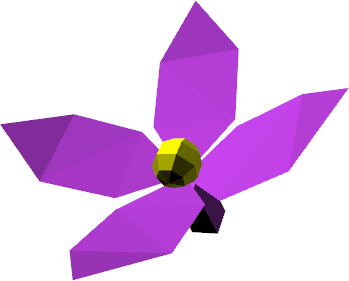
\includegraphics[scale=0.3]{Bloom4}}
	\subfloat[5th iteration]{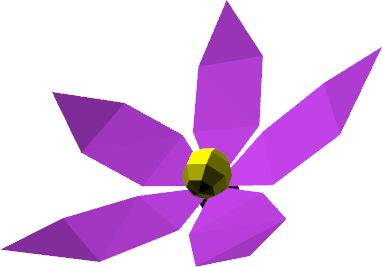
\includegraphics[scale=0.3]{Bloom5}}
	\subfloat[6th iteration]{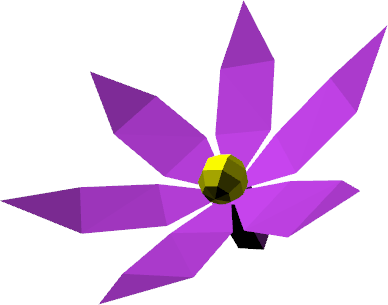
\includegraphics[scale=0.3]{Bloom6}}
	\\
	\subfloat[11th iteration of the Pythagoras tree]{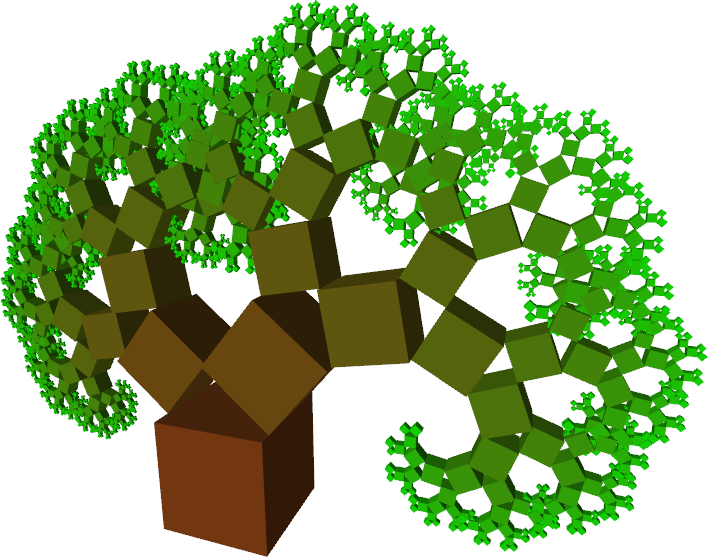
\includegraphics[width=0.55\textwidth]{Pythagoras}} ~
	\subfloat[3rd iteration of the Menger sponge]{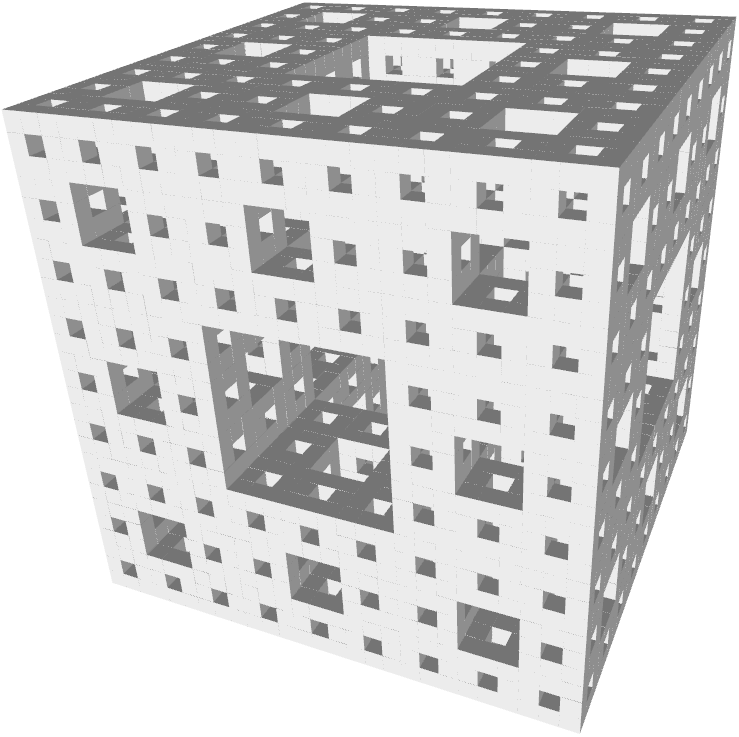
\includegraphics[width=0.40\textwidth]{MengerSponge}}
	\\
	\subfloat[The Pythagoras tree made of the Menger sponges with blossoms at the smallest cubes]{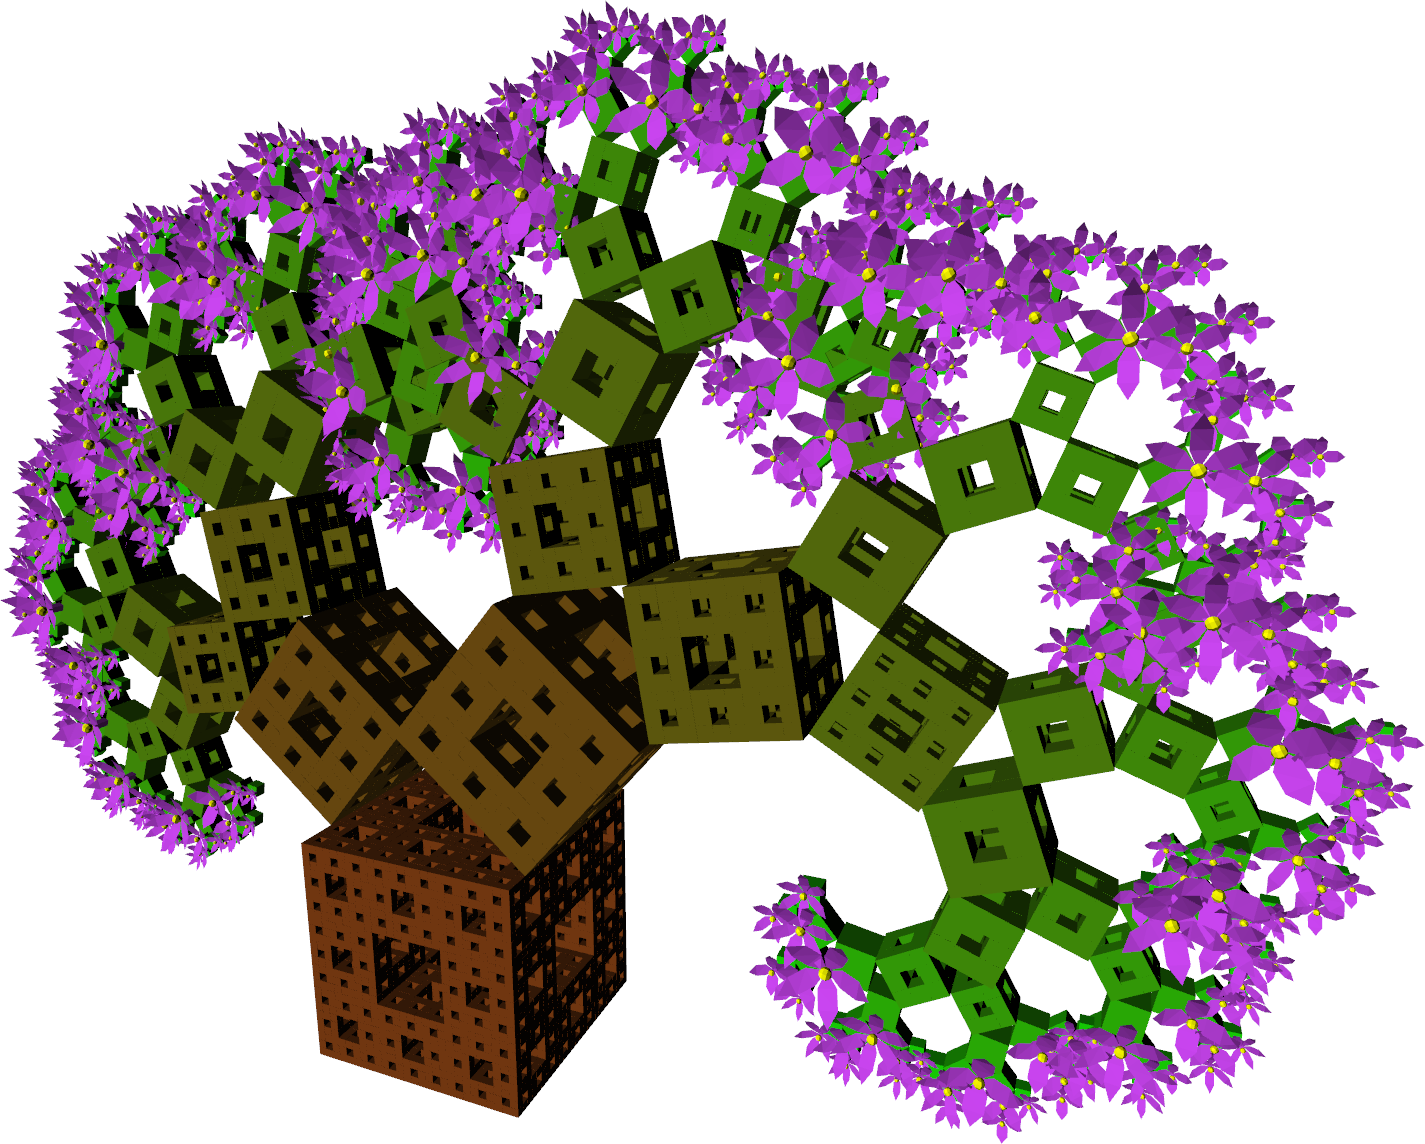
\includegraphics[width=0.9\textwidth]{HybridPythagoras}\label{fig:innerLsystemResult}}
	\caption{Example of interpreting s symbol as another \lsystem}
	\label{fig:innerLsystem}
\end{figure}

\begin{Lsystem}[label=lsys:innerLsystem,caption={Source code of \lsystem (Fig. \ref{fig:innerLsystemResult}) demonstrating use of an interpreting symbol as another \lsystem}]
lsystem HybridPythagorasTree(angle = 50) extends Branches {
	let angleComp = 90 - angle;  // angle complement
	let sinAngle = sin(deg2rad(angle));
	let sinAngleComp = sin(deg2rad(angleComp));
	set iterations = 8;
	set symbols axiom = F(64, 0);
	// interpret E(x) as DrawForward(x, x);  // cube
	@interpret E(x) as lsystem MengerSponge(x);@  // Menger sponge
	interpret m as MoveForward;
	interpret + as Yaw(angle);
	interpret - as Yaw(-angleComp);
	rewrite F(x)
		with left = x * sinAngle, right = x * sinAngleComp
		to E(x) [ + m(left / 2) F(right) ] - m(right / 2) F(left);
}

lsystem MengerSponge(size = 1) extends StdLsystem3D {
	let iters = if(size > 50, 2, if(size > 10, 1, 0));
	let cubeSize = size * (1/3)^iters;
	let renderBlooms = iters == 0;
	// add iteration to render blooms
	let iters = iters + if(renderBlooms, 1, 0);
	set iterations = iters;
	set symbols axiom = F;
	interpret F as DrawForward(cubeSize, cubeSize, #EEEEEE);
	interpret f as MoveForward(cubeSize / 2);
	@interpret B as lsystem Bloom(cubeSize);@  // renderes bloom
	rewrite F where renderBlooms to F [ ^ f B ];
	rewrite F to - f f + & f f ^ F F F +f+f- F F +f+f- F F +f+f- F
		-f+f+f^f F F &f&f^ F F &f&f^ F ^ ^ f f f & + f F F &f&f^ F
		^ ^ f f f & + f F F &f&f^ F ^ ^ f f f & + f F f & f f ^ +
		+ f f - f f f f f;
	rewrite f to f f f;
}

lsystem Bloom(size = 1) extends Polygons {
	let color = #d649ff;
	let leafCount = floor(random(4, 7));
	let angle = 150 / leafCount;
	set iterations = leafCount;
	set symbols axiom = F [ G(size/8) K ] leaf;
	interpret F as DrawForward(size * 0.5, size * 0.2, color);
	interpret G as MoveForward(size * 0.5);
	interpret K as DrawSphere(size / 6, #FFFF00);
	interpret + as Yaw(angle);
	interpret - as Yaw(-angle);
	interpret / as Roll;
	interpret ^ as Pitch(-15);
	rewrite leaf to /(360 / leafCount) [ ^(90) <(color) .
		+ ^ G . - ^ G . - ^ G . + +(180) + G . - ^ G .  > ] leaf;
}

process HybridPythagorasTree with ThreeJsRenderer;
\end{Lsystem}



\subsection{Final component system}

The final component system uses all the described functionality.
The component graph is shown in \autoref{fig:finalSystem}.
Two main \emph{process configurations} defined in the standard library use this scheme, namely the \hyperref[configurationSvgRenderer]{\emph{SvgRenderer}} and the \hyperref[configurationThreeJsRenderer]{\emph{ThreeJsRenderer}}
	(see appendix \ref{sec:stdLibProcessConfigurations}).

\begin{figure}[h!]
	\centering
	\begin{tikzpicture}[->,auto, node distance=3cm,>=latex,shorten >=2pt]
		\node (it) [block] {Iterator};
		\node (in) [block, above of=it, node distance=20mm] {Axiom provider};
		\node (rand) [block, below left of=it, node distance=28.284mm] {Random generator provider};
		\node (rw) [block, left of=it] {Rewriter};
		\node (caller) [block, right of=it, node distance=35mm] {Interpreter caller};
		\node (inter) [block, above of=caller, node distance=20mm] {Interpreter};
		\node (rend) [block, right of=inter] {Renderer};
		\node (out) [coord, right of=rend] {};
		\node (inner) [block, below of=caller, node distance=20mm] {Inner L-system processor};
				
		\draw (rw) to[bend left=40] (it);
		\draw (it) to[bend left=40] (rw);
		\draw (in) -- (it);
		\draw (it) -- (caller);
		\draw (it) -- (rand);
		\draw (caller) -- (inner);
		\draw [dashed] (caller) -- (inter);
		\draw (inter) -- (rend);
		\draw (rend) -- node {output} (out);
	\end{tikzpicture}
	\caption{Final component system}
	\label{fig:finalSystem}
\end{figure}

























\clearpage

\section{Web user interface}

The user interface is very important part of whole project.
To basic forms of user interface was considered, desktop application and web site.
The web was chosen because of following reasons.

\begin{description*}
	\item[Accessibility]
		Web is accessible on wide range of operating systems where desktop application can not be ported easily.
		Besides usual desktop systems it is possible to browse it on mobile devices like smart phones or tablets.		
	\item[No installation]
		End-user do not install anything, the application does not depend on user's OS.
		The solution is not easy to setup because it has many dependencies to third-party libraries.
		Web application is installed by experienced administrator and everything is set up properly.
	\item[Community]
		Users can share and discuss their work on the same place where they create it.
		This helps to create community which is important to all projects.
	\item[Up to date]
		Web user interface is always up to date.
		All updates are instantly applied for all users.
		Errors can be logged and administrator can fix them as soon as possible.		
\end{description*}

\begin{wrapfigure}{r}{0.4\textwidth}
	\vspace{-20pt}
	\includegraphics[width=\linewidth]{Sunflower}
	\caption{Logo of the web}
	\label{fig:logo}
	\vspace{-20pt}
\end{wrapfigure}

Web user interface also serve as comprehensive example of \lsystem processing library and its usage and capabilities.
Sunflower model in \autoref{fig:logo} was produced by the web site and because of its shape which fits in rectangle and good recognizability even as $32 \times 32$ pixels image it was chosen as the logo of the web page.

Web page have four main parts. First three parts, namely \emph{\lsystem processor}, \emph{Gallery of \lsystems} and \emph{Help} are accessible to anyone.
Fourth part is the \emph{Administration} and it is accessible only to administrators.

\subsection{\lsystem processor}

Main functionality of the web is processing of user's input (source code) and showing results.
For this purpose there is web page with big text area where the source code can be written.
There is three possibilities how to submit the source code.

First is processing source code and showing all results (or list of errors).
If there are too many outputs they are packed to one ZIP file.
All results can be downloaded.

Second possibility is to just compile source code and see compiled source code (no results are showed).
This is intended for debugging of errors in the input.

Last possibility which is available only for registered users is to save the source code.
To be able to save the source code successfully it must be without compilation errors.
For each saved source code unique is generated and it can be accessed by permanent link.
Saved inputs can be published in gallery.


\subsection{Gallery of \lsystems}

The gallery will serve as showcase of capabilities of \lsystems for new users as well as learning material.
All entries in gallery will have their source code included and anybody can try to process and customize it.
Registered users can rate other gallery entries.

Every registered user may contribute to gallery with their own creation.
To \lsystem into gallery user have to save and publish source code via \lsystem processor.
It is possible to alter thumbnail \lsystem over original \lsystem.
This allows to simplify images in thumbnail and show complex model in detail.

Tags can be assigned to each \lsystem in gallery.
Tag is short keyword, term or abbreviation which helps to describe \lsystem and allows it to be found again.
List of all tags can be listed and list of \lsystems filtered by specific tag can be shown.
Tag can contain short description of its meaning.
The description can be edited only by special user group.

\lsystems can be filtered also by user name.


\subsection{Help}

Important part of the web is the help.
Help contains few basic topics and FAQ (frequently asked questions) for new users.
Then there is list of predefined components, process configurations, constants, functions and operators.
Last part of the help is detailed syntax reference.


\subsection{Administration}

Administration section of the web is accessible to restricted group of users.
There is more administrators group every with different privileges.

The main administrators group is able to manage roles for all users, manage user groups (roles) and explore error logs.

Next group is able to explore all processed inputs on site, see all saved inputs and export input database to text file.

Last group can see list of submitted feedbacks and if the new feedback is submitted all users from this group will receive it via e-mail.


\subsection{Database}

The database will serve for saving all necessary data.
Figures \ref{fig:dbSchema1} and \ref{fig:dbSchema2} shows database scheme.
\emph{PK} after name means primary key and \emph{FK} foreign key.


\tikzstyle{db} = [draw, fill=blue!12, rectangle split, rectangle split parts=2]
\begin{figure}[p]
	\centering
	\begin{tikzpicture}[auto,>=latex]
		\node (user) [db, text width=6cm] {\textbf{User} \nodepart{second}
			UserId [Int32] (PK)\\
			Name [String] \\
			NameLowercase [String] \\
			PasswordHash [Binary] \\
			PasswordSalt [Binary] \\
			Email [String] \\
			RegistrationDate [DateTime] \\
			LastLoginDate [DateTime] \\
			LastActivityDate [DateTime] \\
			LastPwdChangeDate [DateTime]
		};
			
		\node (feedback) [db, below of=user, node distance=7cm, text width=6cm] {\textbf{Feedback} \nodepart{second}
			FeedbackId [Int32] (PK) \\
			UserId [String] (FK) \\
			Subject [String] \\
			SubmitDate [DateTime] \\
			Email [String] \\
			Message [String] \\
			IsNew [Bool]
		};
			
		\node (role) [db, above of=user, node distance=6cm, text width=6cm] {\textbf{Role} \nodepart{second}
			RoleId [Int32] (PK) \\
			Name [String] (FK) \\
			NameLowercase [String]
		};		
		
		\node (x) [coord, above right of=user, node distance=8cm] {};
		
		\node (vote) [db, above of=x, node distance=4cm, text width=6cm] {\textbf{Saved input vote} \nodepart{second}
			SavedInputId [Int32] (PK) \\
			UserId [Int32] (PK) \\
			Rating [Int32]
		};
		
		
		\draw [<-] (user) -- (feedback) node[pos=0.2]{0..1}  node[pos=0.55]{UserId}  node[pos=0.85]{*};
		\draw (role) -- (user) node[pos=0.2]{*}  node[pos=0.8]{*};
		\draw (vote) -- (x) node[pos=0.2]{*};
		\draw [->] (x) -- (user) node[pos=0.5]{UserId}  node[pos=0.8]{1};
		
		\draw [->] (x.east) -- +(3cm,0)  node[below,pos=0.5]{SavedInputId}  node[pos=0.8]{1}   node [xshift=1.5cm] {Saved inputs};
		\draw [<-] (user.east) ++(0,1cm) -- +(4cm,0) node[pos=0.2]{1}  node[below,pos=0.5]{CreationUserId}  node[pos=0.8]{*}   node [xshift=1.5cm] {Saved inputs};
		\draw [<-] (user.east) ++(0,-2cm) -- +(4cm,0) node[pos=0.2]{0..1}  node[below,pos=0.5]{UserId}  node[pos=0.8]{0..1}   node [xshift=1.5cm] {Input process};
		
	\end{tikzpicture}
	\caption{First half of the database scheme of the web}
	\label{fig:dbSchema1}
\end{figure}

\begin{figure}[p]
	\centering
	\begin{tikzpicture}[auto,>=latex]
		\node (input) [db, text width=6.5cm] {\textbf{Saved inputs} \nodepart{second}
			SavedInputId [Int32] (PK)\\
			UrlId [String] \\
			ParentInputProcessId [Int32] (FK) \\
			CreationUserId [Int32] (FK) \\
			CreationDate [DateTime] \\
			EditDate [DateTime] \\
			IsPublished [Bool] \\
			IsDeleted [Bool] \\
			PublishName [String] \\
			Views [Int32] \\
			SourceSize [Int32] \\
			OutputSize [Int64] \\
			Duration [Int64] \\
			MimeType [String] \\
			SourceCode [String] \\
			ThumbnailSourceExtension [String] \\
			Description [String] \\
			OutputMetadata [Binary] \\
			OutputThnMetadata [Binary] \\
			RatingSum [Int32] \\
			RatingCount [Int32]
		};
			
		\node (tag) [db, left of=input, node distance=7.5cm, text width=4.5cm] {\textbf{Tag} \nodepart{second}
			TagId [Int32] (PK) \\
			Name [String] \\
			NameLowercase [String] \\
			Description [String]
		};
			
		\node (proc) [db, below of=input, node distance=10cm, text width=6.3cm] {\textbf{Input process} \nodepart{second}
			InputProcessId [Int32] (PK) \\
			ParentInputProcessId [Int32] (FK) \\
			ChainLength [Int32] \\
			CanonicInputId [Int32] (FK) \\
			UserId [Int32] (FK) \\
			ProcessDate [DateTime] \\
			Duration [Int64]
		};
		
		\node (output) [db, below of=proc, node distance=6cm, text width=6cm] {\textbf{Process output} \nodepart{second}
			ProcessOutputId [Int32] (PK) \\
			InputProcessId [Int32] (FK) \\
			FileName [String] \\
			CreationDate [DateTime] \\
			LastOpenDate [DateTime] \\
			Metadata [Binary]
		};
		
		\node (canonic) [db, xshift=-1cm,  below left of=proc, node distance=8.5cm, text width=5.3cm] {\textbf{Canonic input} \nodepart{second}
			CanonicInputId [Int32] (PK) \\
			Hash [Int32] \\
			SourceCode [String] \\
			SourceSize [DateTime] \\
			OutputSize [DateTime]
		};
		
		
		\draw (input) -- (tag)  node[pos=0.2]{*}  node[pos=0.8]{*};
		\draw [->] (input) -- (proc)  node[pos=0.2]{*}  node[pos=0.5]{ParentInputProcessId}  node[pos=0.8]{0..1};
		\draw [<-] (proc) -- (output)  node[pos=0.2]{0..1}  node[pos=0.6]{InputProcessId}   node[pos=0.9]{*};
		\draw [->] (proc) -- (canonic)  node[pos=0.08]{*}  node[pos=0.35]{CanonicInputId}   node[pos=0.65]{1};
		\draw [->] (proc) edge [in=180,out=190,loop] node[pos=0.15]{0..1}  node[pos=0.5]{ParentInputProcessId}   node[pos=0.9]{*} ();
		
		\draw [<-] (input.west) ++(0,4cm) -- +(-4cm,0) node[above,pos=0.2]{1}  node[below,pos=0.5]{SavedInputId}  node[above,pos=0.8]{*}   node [xshift=-2cm] {Saved input vote};
		\draw [->] (input.west) ++(0,-4cm) -- +(-4cm,0) node[above,pos=0.2]{1}  node[below,pos=0.5]{CreationUserId}  node[above,pos=0.8]{*}   node [xshift=-1cm] {User};
		\draw [->] (proc.west) ++(0,1cm) -- +(-4cm,0) node[above,pos=0.2]{0..1}  node[below,pos=0.5]{UserId}  node[above,pos=0.8]{0..1}   node [xshift=-1cm] {User};
	\end{tikzpicture}
	\caption{Second half of the database scheme of the web}
	\label{fig:dbSchema2}
\end{figure}


In the left part of the scheme (\autoref{fig:dbSchema1}) are tables \emph{User} and \emph{Roles} with relation \emph{n} to \emph{n} (any user can be in any number of roles).
both tables table contains column called \emph{NameLowercase} for canonical representation of user names for easier searching.
\emph{Feedback} table for saving posted feedback have foreign key to \emph{Users} (if registered user submit a feedback).

The right part of the scheme is (\autoref{fig:dbSchema2}) more complicated.
Every processed input is saved to the \emph{Input process} table.
To optimize size of the database the source code is not saved for every input process but it is canonicalized and saved to the \emph{Canonic input} table.
Hash is counted for every saved canonical input to speed up lookup for identical inputs.
This system ensures that in the database will not be saved two identical source codes.
One might thing that the probability of processing two identical source codes is very low but it is not true.
The most users trying to process \lsystems from gallery and do minor changes to them like changing number of iterations.

Results of processing (like images) are not saved directly to database because they are relatively big.
They are saved to local disk to working directory (which can be configured).
To ensure correct cleaning of files in the working directory there is table called \emph{Process output}.
Record of each produced file is saved into this table.
If file is viewed by user the \emph{LastOpenDate} entry is updated.
If the number of stored files exceeds maximum (which can be configured) the files with the longest time before last opening are deleted.
This mechanism allows to keep alive old but viewed files with no need to saving them permanently (for example for sharing with friend).

Moreover the new files are saved with the \emph{LastOpenDate} lowered by one minute over the \emph{CreationDate}.
This will cause that deleting of non-viewed files is likely than viewed ones.
It can protect wiping all input from database by some bot who do not open processed outputs.

Lets get back to saving of all processed inputs to the \emph{Input process} table.
If user is creating \lsystem the process is iterative.
Parent input processes are saved (in \emph{ParentInputProcessId}) as user develops the \lsystem.
This set of processes forms a chain.
The longer the chain of processes is the better can be expected.
The length of a chain can be counted by searching the database an resolving the \emph{ParentInputProcessId} column.
However this process can take very long time because the \emph{Input process} table will likely have many rows.
To be possible to easily find longest chains the chain length is counting for each row in column \emph{ChainLength}.

If new input is about to save to the \emph{Input process} table and it do not have parent (for example first process after opening the page) the \emph{Canonic input} table is searched for corresponding input.
If the canonical input it is found the oldest\footnote{More input process entries can share one canonical input entry.} corresponding input process is selected as the parent.


\subsubsection{Saved inputs}

Registered users can save their inputs.
They are saved to the \emph{Saved inputs} table which also serves as table for the gallery.
For every saved input is generated unique ID stored in the \emph{UrlId} column.
This is is used in the permanent link which allows permanent access to all saved inputs.

Saved inputs can be edited by owner but more importantly the can be published to the gallery.
In the gallery inputs can be rated.
For this is table \emph{Saved input vote}.
Primary key to this table is pair of \emph{SavedInputId} and \emph{UserId} allowing each user to vote to every input just once (of course the vote can be changed).

Published entries in the \emph{Saved inputs} table are sorted by average rating taking into account total number of votes (the more votes the better).
To speed the sorting and eliminate joining with the \emph{Saved input vote} table the sum and the count of votes is stored directly in the \emph{Saved inputs} table.

Source code of saved inputs is saved as is (without any canonicalization) to preserve comments and formatting.
To allow generating thumbnail different from the original image and to save space and user effort the thumbnail is generated by adding content of the \emph{ThumbnailSourceExtension} to the \emph{SourceCode}.
Because the last result is saved the source code in the \emph{ThumbnailSourceExtension} can produce thumbnail easily with usage of next process statement.

























































\chapter{Implementation}
\label{chap:implementation}

In this chapter will be described implementation of designed system.
[TODO]


\section{Choice of development environment}

As development environment was chosen .NET because of following reasons.

\begin{description*}
	\item[Multiplatformity]
		Thanks to Mono project\footnote{Mono is an open source implementation of Microsoft's .NET Framework \url{http://www.mono-project.com}}
			.NET libraries and executables can be used not only on Windows but also on Linux, Mac and many other operating systems.
	\item[Development tools]
		Visual Studio is powerful integrated development environment (IDE) with many integrated tools (like inteli-sense, unit testing or T4 templates) and useful downloadable plugins.
	\item[Reflection]
		Reflection is the ability to examine types and work with meta-data, properties and functions of an object at runtime.
		Reflection can be used to load various plugins or data at runtime and help extensibility in great way.
	\item[Parser generator]
		FsLex and FsYacc are lexer and parser generators written in F\# with good support by Visual Studio.
		Generated lexer and parser are also in F\# thus they can be easily used in any .NET project.
	\item[Web framework]
		ASP.NET MVC is a lightweight presentation framework for creating web applications in .NET.
\end{description*}

The most of code will be written in C\# expect input lexer and parser which will be in F\#. 


\section{Solution structure}

The solution is divided into 6 projects: \lsystem processing library (Malsys), web user interface (Malsys.Web), abstract syntax tree (Malsys.Ast), syntax parser (Malsys.Paring), common functionality (Malsys.Common) and project with tests (Malsys.Tests).

The main reason why solution do not contain lower amount of projects is because syntax parser is written in F\# which is also language from .NET family but it is not possible to compile F\# and C\# into single DLL.
Abstract syntax tree (AST) is separated from parser because AST will be compiled by compilers written in C\# and it is desirable to have AST data structures written in C\#.
It is also more comfortable to design AST classes in C\# because F\# is functional language and syntax of classes definition is quite complex.
Common functionality is separated into single project because it will be needed in all projects and solution can not have circular dependencies of projects.
Web project is separated from main project intentionally to allow usage of \lsystem processing library independently.
And finally test project is separated to be possible to test all projects independently.
Dependencies of projects in solution are shown in the Figure \ref{fig:solutionDependencies}.

\begin{figure}[h]
	\centering
	\begin{tikzpicture}[auto, node distance=1cm,>=latex']
		\node (c) [block] {Malsys.Common};
		\node (m) [block, below=of c] {Malsys};
		\node (a) [block, right=of m] {Malsys.Ast};
		\node (p) [blockx, right=of a] {Malsys.Parsing};
		\node (w) [block, left=of m] {Malsys.Web};
		\node (t) [block, below=of m] {Malsys.Tests};
		\node (cSharp) [block, minimum width=1em, minimum height=1em, below=1.5cm of p] {C\#};
		\node (fSharp) [blockx, minimum width=1em, minimum height=1em, right=0.5cm of cSharp] {F\#};
		
		\draw [->] (a) edge node {} (c);
		
		\draw [->] (p) edge[bend right=10] node {} (c);
		\draw [->] (p) edge node {} (a);
		
		\draw [->] (m) edge node {} (c);
		\draw [->] (m) edge[bend right] node {} (p);
		\draw [->] (m) edge node {} (a);
		
		\draw [->] (w) edge[bend left=20] node {} (c);
		\draw [->] (w) edge node {} (m);
		\draw [->] (w) edge[bend right=25] node {} (a);
		
		\draw [->] (t) edge[bend left=56] node {} (c);
		\draw [->] (t) edge node {} (m);
		\draw [->] (t) edge[bend right=20] node {} (p);
		\draw [->] (t) edge[bend right=20] node {} (a);
		\draw [->] (t) edge[bend left=20] node {} (w);
	\end{tikzpicture}
	\caption{Dependencies of projects in solution}
	\label{fig:solutionDependencies}
\end{figure}




[TODO]
%Input source code needs to be parsed to \emph{abstract syntax tree} further called AST.
%Generally there are two approaches how to parse it.
%Write parser from scratch or use third-party parser generator.
%Because syntax is 























\chapter{Results}

This section summarizes results

\section{Web user interface}

\begin{wrapfigure}{r}{0.4\textwidth}
	
\includegraphics[width=\linewidth]{malsys_cz}
	\caption{\url{http://malsys.cz}}
	\label{fig:malsysQr}
\end{wrapfigure}

The web user interface was deployed and it is accessible at address \emph{http://malsys.cz}.
The main function of the web is to process \lsystems.
Detailed instructions can be found in appendix \ref{chap:userDoc}.
Web site includes \lsystem gallery and help.

Any user can register and gain some advantages.
Registered users can save and publish their \lsystems to public gallery and they have longer time limit for processing of \lsystems.

Web page is displayed correctly in the most common web browsers namely Google Chrome, Opera, Firefox, Internet Explorer and Safari.
It is possible to browse it in smart phones or tablets.
\autoref{fig:galleryInDevices} shows print-screens of the first page of the gallery on various operating systems.
Web page is supports pinning to Windows taskbar (\autoref{fig:pinIe}). 

\begin{figure}[h]
	\centering
	\subfloat{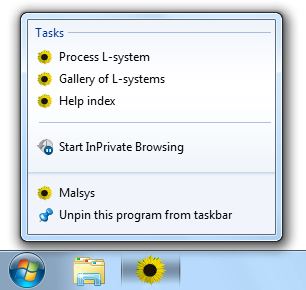
\includegraphics[scale=0.5]{JumpList}} ~
	\subfloat{
\includegraphics[scale=0.5]{PinnedIeHeader}}
	\caption{Jump-list of pinned site and header of opened Internet Explorer 9 using pinned shortcut}
	\label{fig:galleryInDevices}
\end{figure}


\begin{figure}[p]
	\centering
	\subfloat[Windows 7 (Google Chrome)]{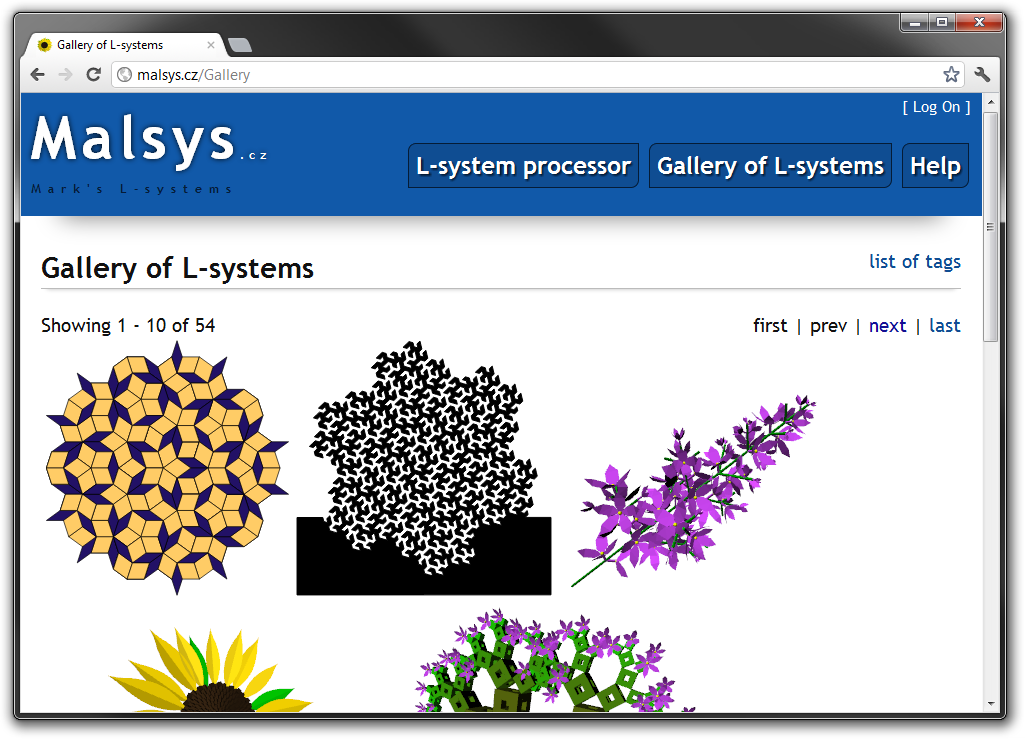
\includegraphics[width=\linewidth]{GalleryInChrome}}
	\\
	\subfloat[Android OS (Firefox)]{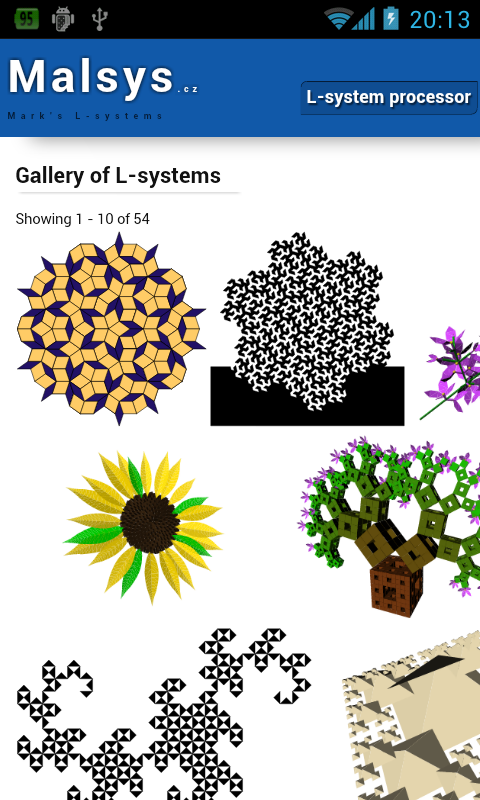
\includegraphics[height=7cm]{GalleryOnAndroid}} ~
	\subfloat[Windows Phone (IE9 mobile)]{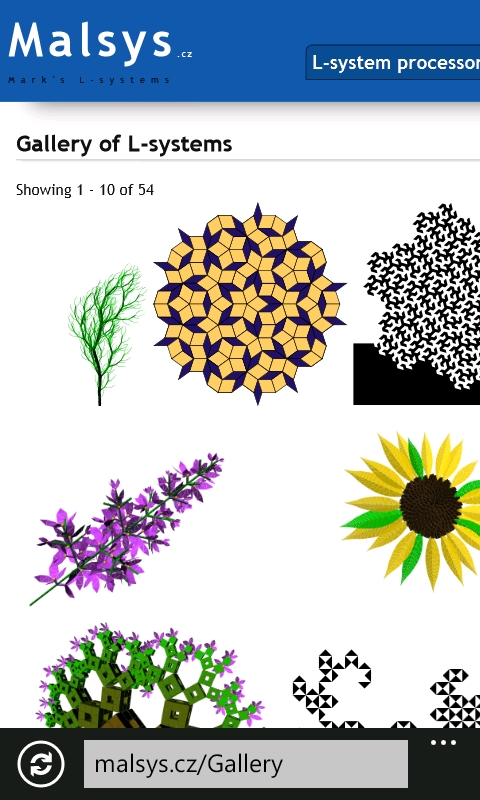
\includegraphics[height=7cm]{GalleryOnWindowsPhone}} ~
	\subfloat[Amazon Kindle 3]{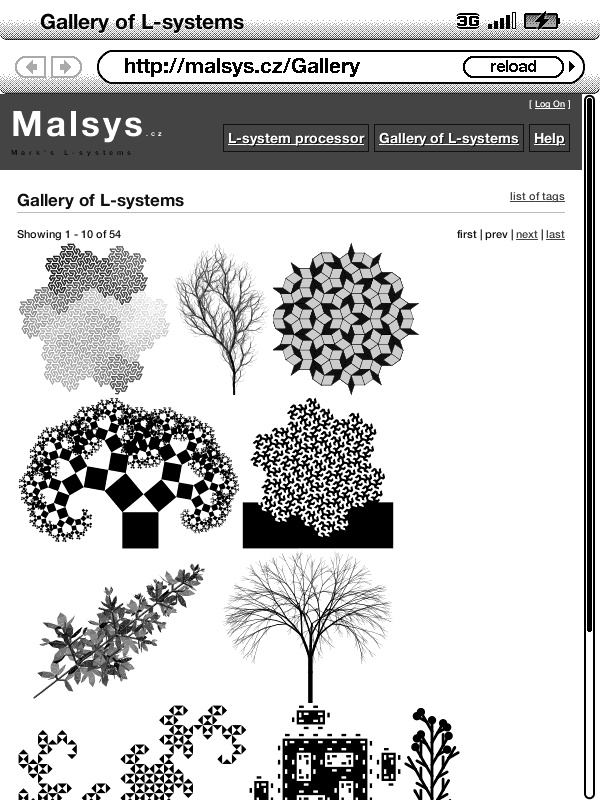
\includegraphics[height=7cm]{GalleryOnKindle}}
	\caption{The first page of the gallery displayed on various operating systems}
	\label{fig:pinIe}
\end{figure}


\subsection{Visitors and traffic}

The web was officially released on 15 April 2012.
Two days later it was posted some notifications on Twitter and Facebook.
This day number of visitors peeked at 142 but most of them just checked the gallery and next day the the messages on social networks were lost.

About week after initial release short newsflash was posted on Czech server \url{http://root.cz} which attracted 255 visitors that day.
But visitors from the root.cz was not just looking in the gallery.
In the contrast with visitors from social networks users from the root.cz started to experiment with \lsystems.
This was probably because of fact that the root.cz is the a site about computer technologies, software and programming and users understood \lsystems better.

At the end of May, one and half months after initial release malsys.cz was seen by over 1000 unique visitors and they browsed over 9000 pages.


\section{Showcase of \lsystems}

The most \lsystems is used in this thesis as figures illustration described themes.
In this section are images of some more \lsystems.

\begin{figure}[h]
	\subfloat{
		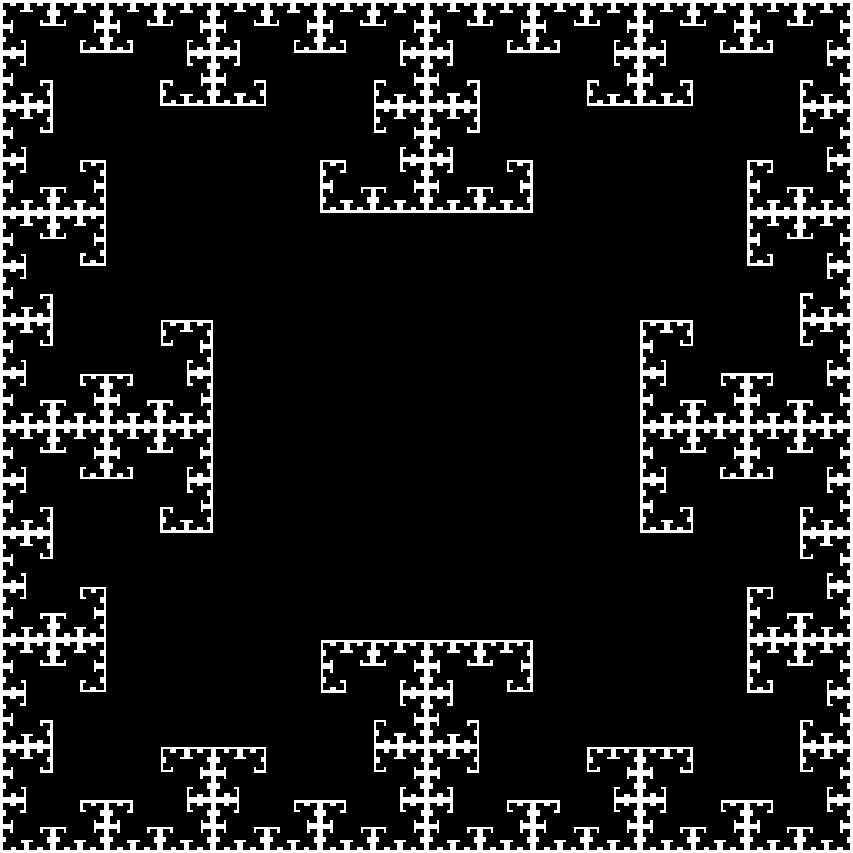
\includegraphics[width=0.49\linewidth]{Tsquare}
		\label{fig:introLilac}
	} \hfill
	\subfloat{
		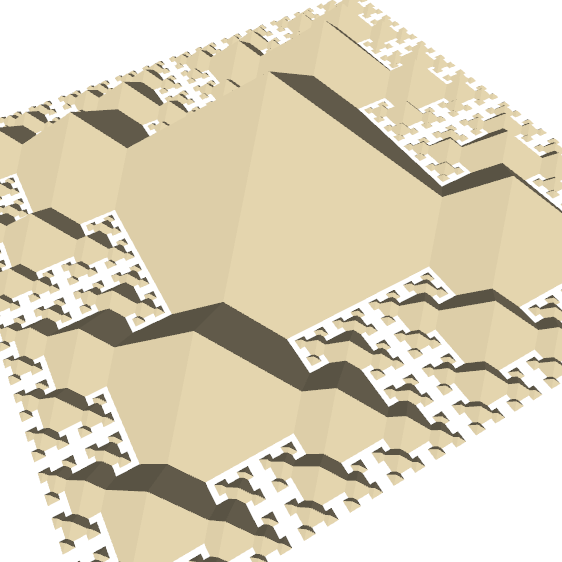
\includegraphics[width=0.49\linewidth]{Tsquare3D}
		\label{fig:introHTree}
	}
	\caption{T-square fractal (left) and its generalization to 3D with pyramids instead of squares (right)}
\end{figure}

\begin{figure}[h]
	\subfloat{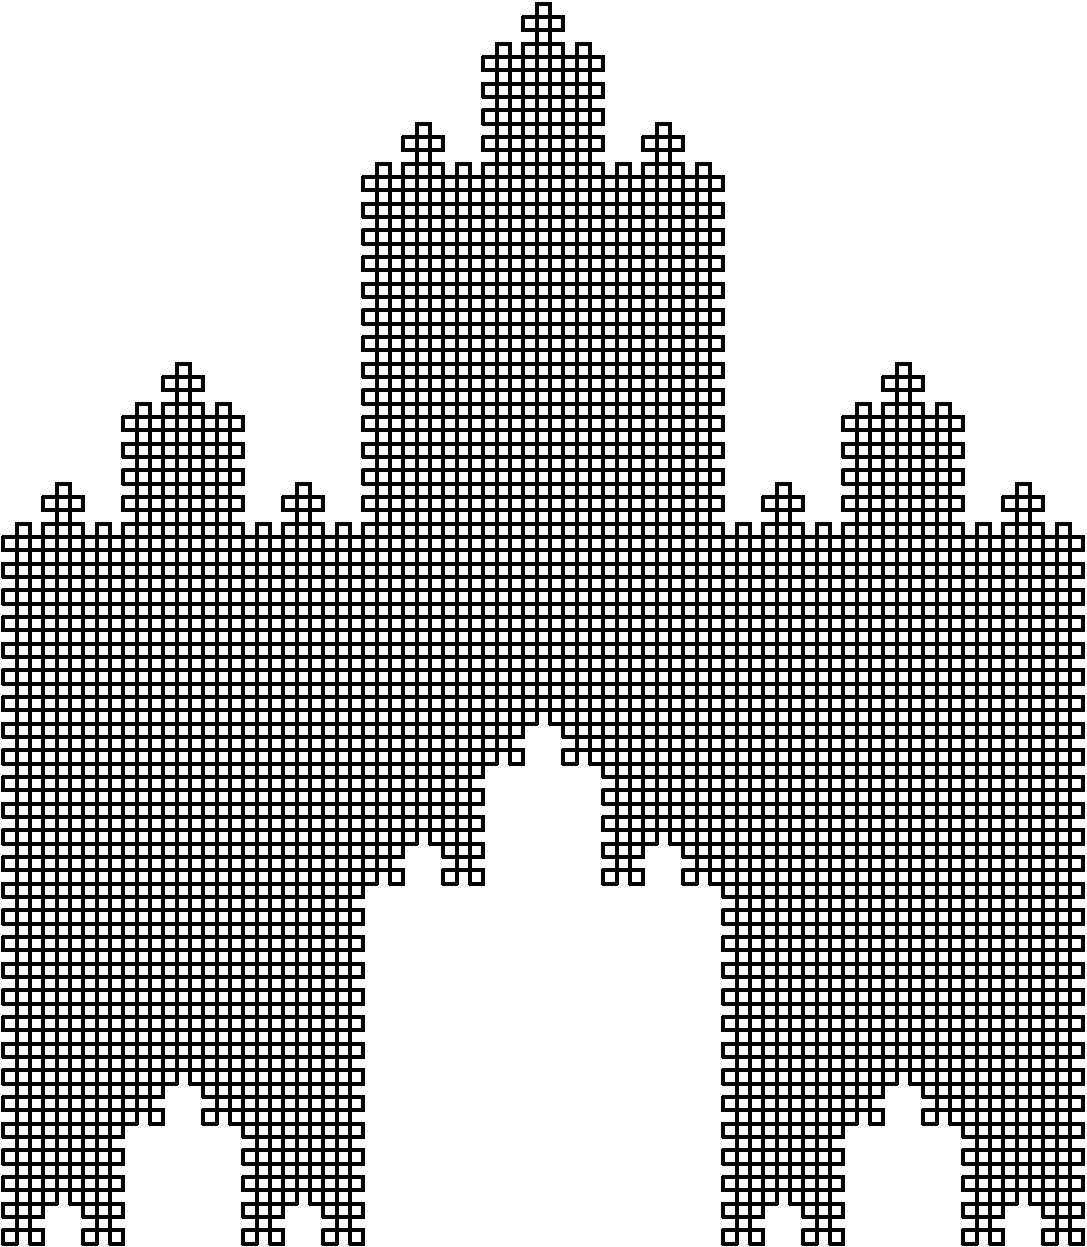
\includegraphics[width=0.49\linewidth]{DekkingsChurch}}
	\hfill
	\subfloat{
\includegraphics[width=0.49\linewidth]{HilbertCurve}}
	\caption{Dekking's chirch (left) and Hilbert curve (right)}
\end{figure}

\begin{figure}[p]
	\centering
	\subfloat{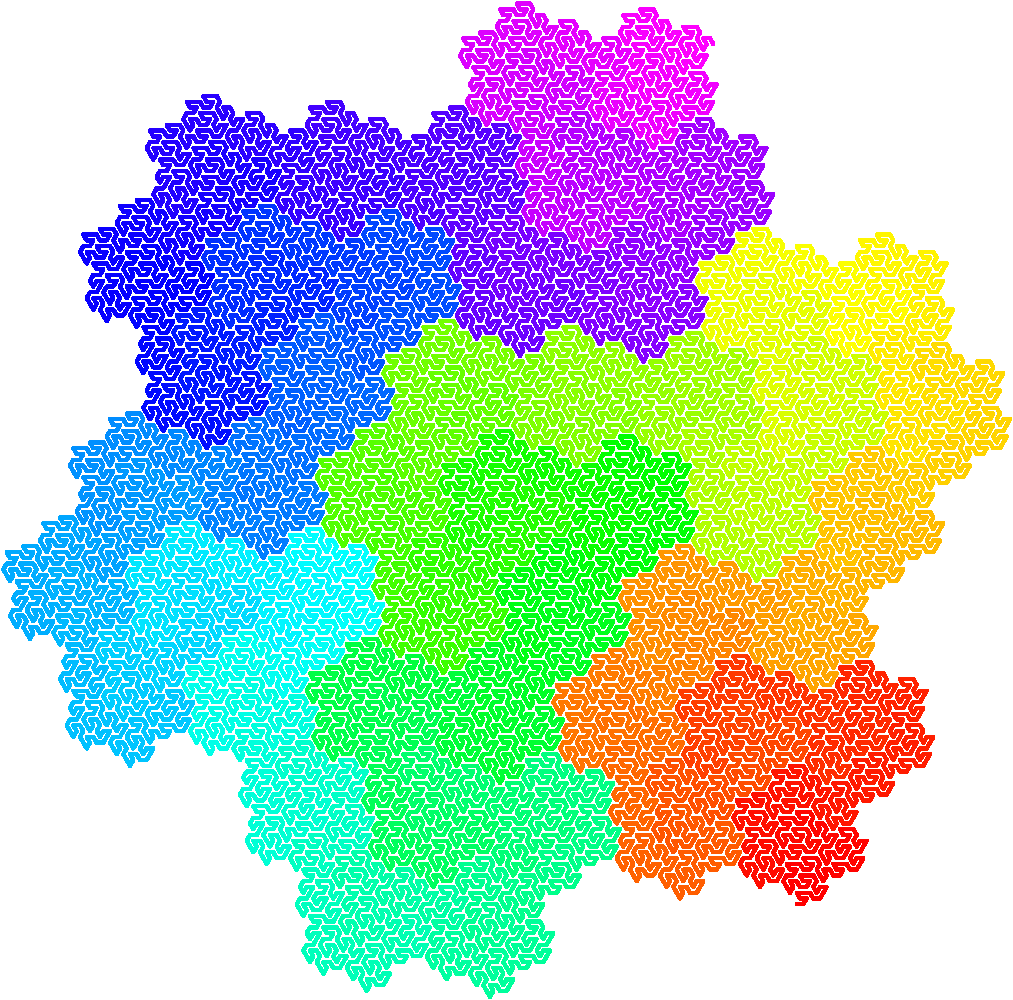
\includegraphics[width=	\linewidth]{HexaGosper}}
	\caption{Hexagonal Gosper curve}
\end{figure}

\newsavebox{\lstBoxGosper}
\begin{lrbox}{\lstBoxGosper}
\consolas
\footnotesize
\begin{lstlisting}
            ________          
            \       \         
  ________   \____   \        
  \       \      /   /        
   \____   \____/   /   ____  
       /            \   \   \ 
  ____/   ________   \   \   \
 /        \       \   \  /    
/   ____   \____   \   \/     
\   \   \      /   /          
 \   \   \____/   /   ____    
  \  /            \  /   /    
   \/   ________   \/   /     
        \       \      /      
         \____   \____/       
             /                
        ____/                 
\end{lstlisting}
\end{lrbox}

\begin{figure}[p]
	\subfloat{
		\minipage{0.47\linewidth}\noindent
			
\includegraphics[width=\linewidth]{HexaGosperFilled}
		\endminipage
	}
	\hfill
	\subfloat{
		\usebox{\lstBoxGosper}
	}
	\caption{Hexagonal Gosper curve as polygon (left) and as ASCII art (right)}
\end{figure}

\begin{figure}[p]
	\centering
	\subfloat{
\includegraphics[width=\linewidth]{IslandsAndLakes}}
	\caption{Islands and lakes}
\end{figure}

\begin{figure}[p]
	\subfloat{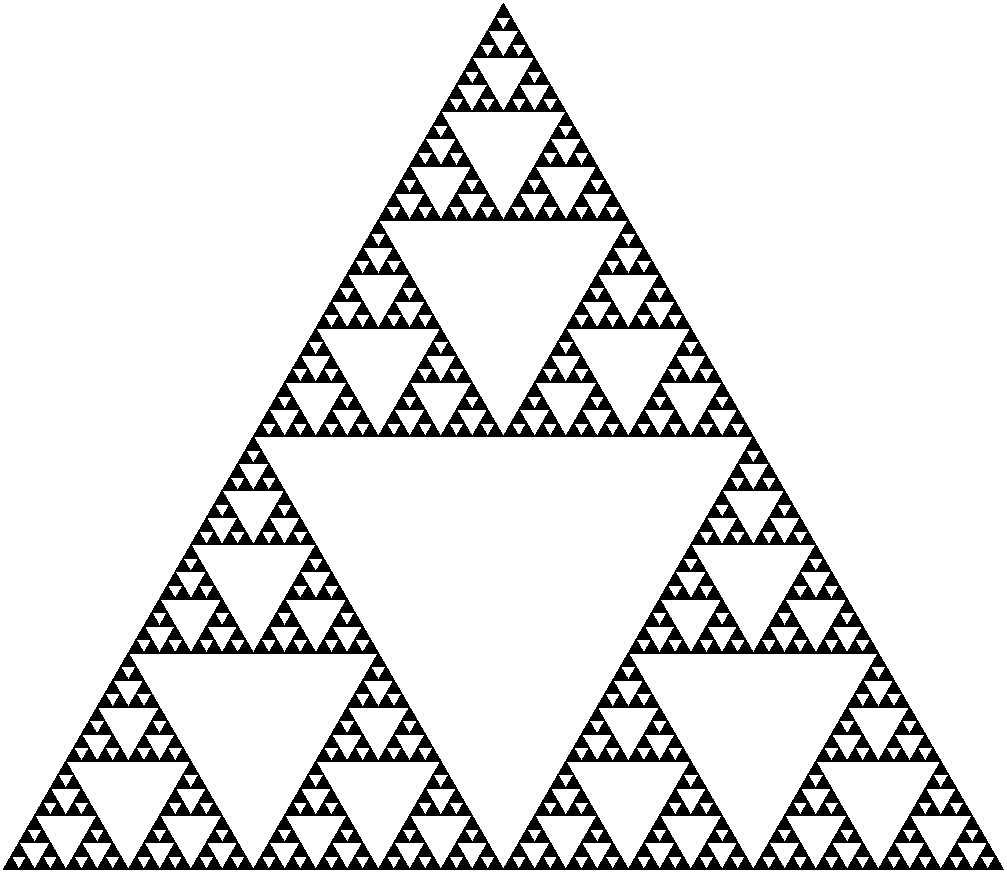
\includegraphics[width=0.49\linewidth]{SierpinskiTriangle}}
	\hfill
	\subfloat{
\includegraphics[width=0.49\linewidth]{SierpinskiTriangleI}}
	\caption{Basic (left) and inverted (right) Sierpinski triangles}
\end{figure}

\begin{figure}[p]
	\centering
	\subfloat{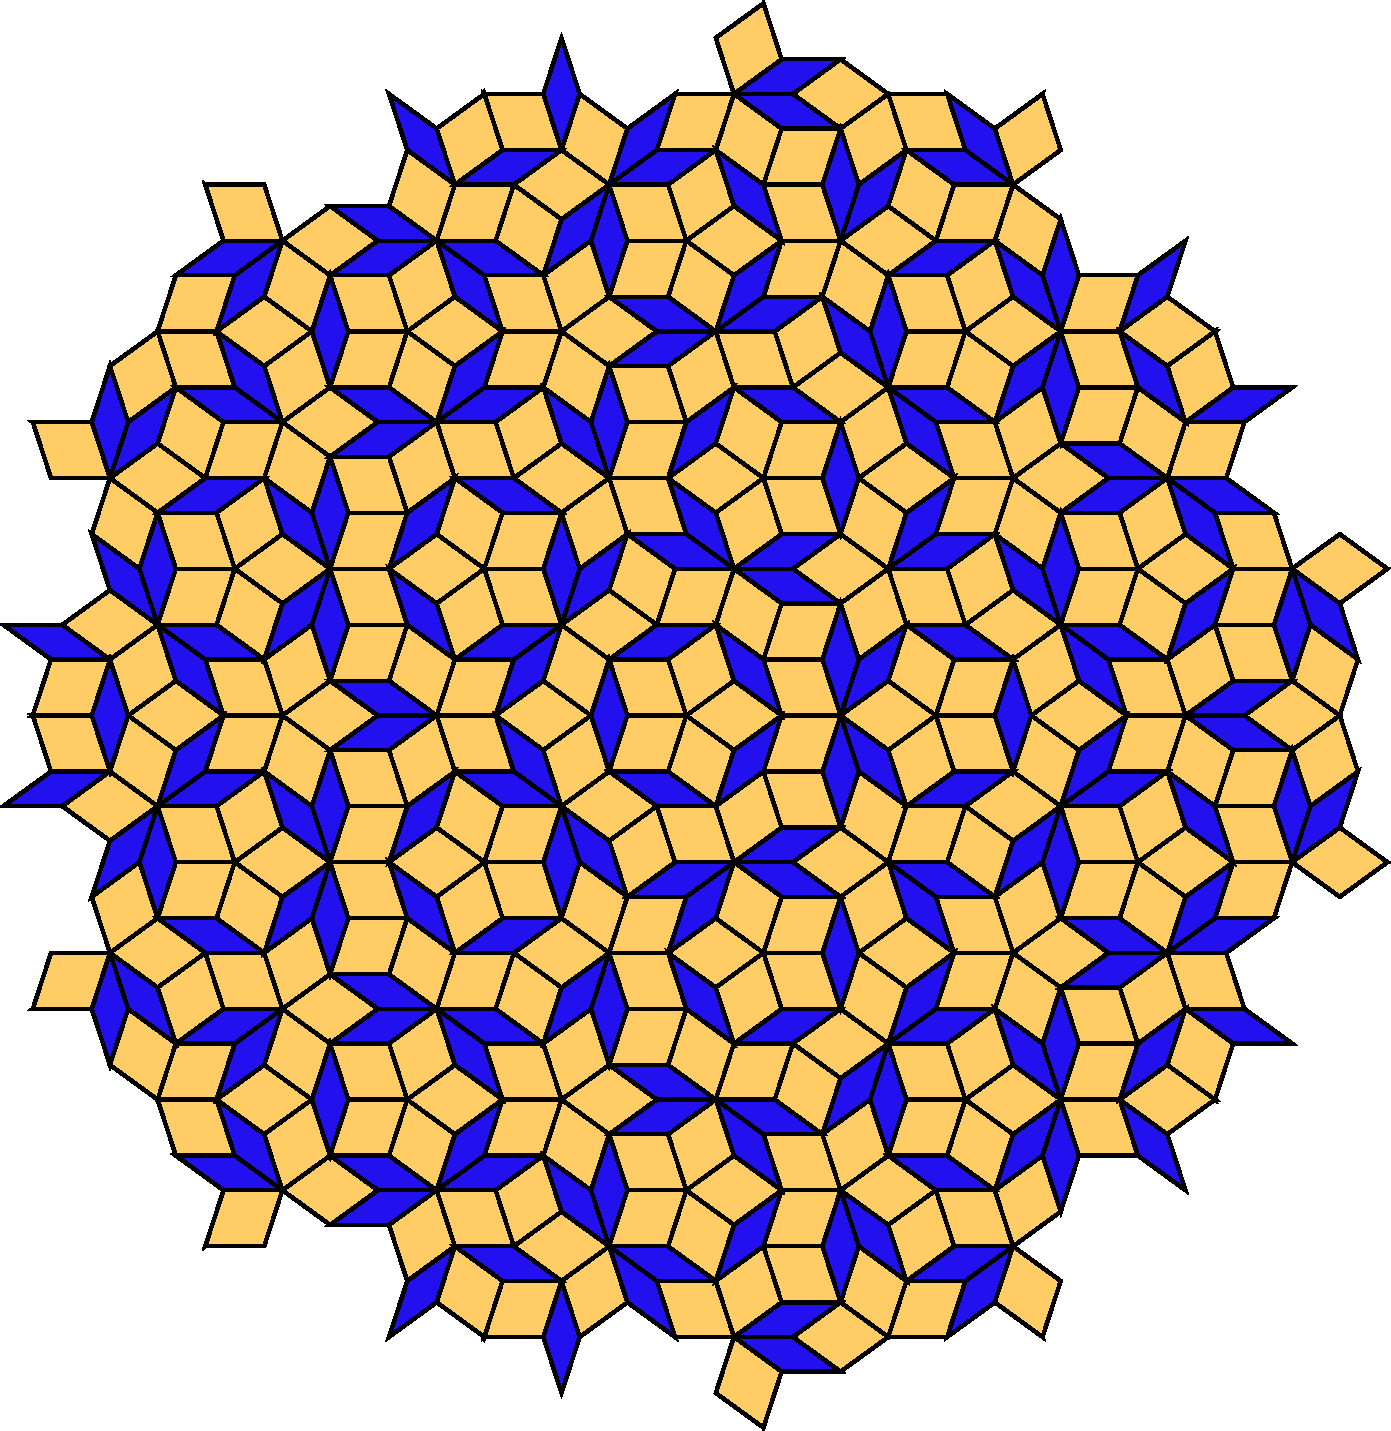
\includegraphics[width=\linewidth]{PenroseTiling}}
	\caption{Penrose tiling}
\end{figure}

\begin{figure}[p]
	\subfloat{\includegraphics[width=0.40\linewidth]{Circles}}
	\hfill
	\subfloat{\includegraphics[width=0.58\linewidth]{Circles3D}}
	\caption{Circles (left) and its generalized version in 3D (right)}
\end{figure}

\begin{figure}[p]
	\centering
	\subfloat{\includegraphics[width=\linewidth]{LilacHuge}}
	\caption{Lilac panicle}
\end{figure}

\begin{figure}[p]
	\centering
	\subfloat{\includegraphics[width=\linewidth]{SunFlowerHuge}}
	\caption{Sunflower}
\end{figure}

\begin{figure}[p]
	\subfloat{\includegraphics[width=0.28\linewidth]{Plant1}}
	\hfill
	\subfloat{\includegraphics[width=0.36\linewidth]{Dandelion}}
	\hfill
	\subfloat{\includegraphics[width=0.25\linewidth]{Plant2}}
	\caption{Models of plant-like structures with withered dandelion in the middle}
\end{figure}



\section{Solution statistics}

\autoref{tbl:stats} shows number of lines of code written by hand based on file types.
Listed numbers do not include generated code (if not stated otherwise).
Also note that help pages with \emph{predefined stuff} in the web are generated dynamically thus their content is not included in statistics of total line count.


\begin{table}[h]
	\centering
	\begin{tabular}{p{65pt} c c p{200pt}}
   		\toprule
   		Extension & Type & Line count & Comment\\
   		\midrule
		.cs & C\# & > 30 000 &  \\ \hline
		.fs, .fsy, .fls & F\# & > 1 000 & F\# files together with lexer and parser definitions \\ \hline
		.cshtml & Razor & > 10 000 & views of the razor view engine\\ \hline
		.generated.cs, .designer.cs & C\# & > 5 000 & automatically generated files \\ \hline
		\bottomrule
	\end{tabular}
	\caption{Number of lines of code written by hand (if not stated otherwise) based on file types}
	\label{tbl:stats}
\end{table}


























\chapwithtoc{Conclusion}

The goal of this work was to create online feature-rich development environment for anybody who wants to experiment with \lsystems.
This goal was achieved and the result can be seen at \url{http://malsys.cz}.
However it was created more than just web based \lsystem generator.

\begin{wrapfigure}{r}{0.5\textwidth}
	\includegraphics[width=\linewidth]{HexaGosperNeedlework}
	\caption{Needlework of Hexa-Gosper curve}
	\label{fig:HexaGosperNeedlework}
\end{wrapfigure}

As part of the solution was created standalone modular \lsystem processing library which process \lsystems with component-based system.
Component system and configuration of individual components is defined in the input together with \lsystems.
Components can be created or extended by user which brings great extensibility to \lsystem processing.
Many components are already part of the library.
They are used on the web to process \lsystems and produce 2D images and 3D scenes or even ASCII art.

Component is piece of program thus it can do anything.
For example it is possible to create special component which will interpret \lsystem symbols as commands for some CNC%
	\footnote{CNC stands for Computer Numerical Control and refers specifically to a computer \emph{controller} which drives the powered mechanical device
		which for instance uses number of different tools-drills, saws, etc. for fabricating materials like metal or wood.} 
	sewing machine which can sew an ornament on T-shirt, carpet or curtain (\autoref{fig:HexaGosperNeedlework}).
If stochastic \lsystem will be used no two T-shirts will have the same ornament on it.
This example is relatively bizarre but it reflects extensibility of the library well.

Part of the created web interface is the gallery of \lsystems with more than 50 inserted \lsystems (in time of publishing this thesis) and it is slowly becoming unique database of all basic \lsystems.
Any registered user can save their \lsystems and publish them to the gallery.
Published \lsystems can be rated.


\section*{Future work}

Web user interface does not provide any way for communication between users.
A great improvement will be possibility to add comments to the gallery entries and write personal messages to other users.
Also some simple forum could be helpful.

The \lsystem processing library was written with emphasis on functionality and simplicity, not the performance.
The performance for processing \lsystem on the web is sufficient because it is even not possible to display large outputs in web browsers.
However there are many areas where improvements can be made.
For example compiler can optimize expression trees to eliminate static expressions ($1 + 2 \rightarrow 3$).

Because of component-based design of the \lsystem processing library it is possible to extend it with minimal effort.
The plan was to create renderer which renderes the scene with the PovRay ray-tracer but there was no time for it.

The syntax parser has poor error recovery which should be improved.
Some syntax errors even do not show their position.

































\nocite{*}  % Show all Bib-entries
\printbibliography

%\addcontentsline{toc}{chapter}{List of Figures}
%\listoffigures

%\addcontentsline{toc}{chapter}{List of Tables}
%\listoftables

%\addcontentsline{toc}{chapter}{List of source codes}
%\lstlistoflistings


\openright
\begin{appendices}


\chapter{Contents of attached CD}
\label{chap:attachedCd}




\chapter{Input syntax reference}
\label{chap:syntax}

This appendix contains formal definition of the designed syntax.
The syntax is described with the regular expressions which are explained in the first section.
The syntax is described from the most general parts to more concrete parts.

\section{Regular expressions}
\label{sec:regexps}

Table \ref{tbl:regexpExplanation} explains the syntax of the regular expressions used for description of the input syntax.

\begin{table}[ht]
	\centering
	\begin{tabular}{c p{160pt} p{170pt}}
   		\toprule
   		Regexp & Definition & Example \\
   		\midrule
		\texttt{' '} & matches the text between quotes (and nothing else) & \texttt{'let'} matches only string \texttt{let} \\ \hline
		\texttt{[ ]} & matches one of any characters enclosed in brackets & \texttt{[ab]} matches only \texttt{a} or \texttt{b} \\ \hline
		\texttt{[ - ]} & matches single character between two specified characters (inclusive) & \texttt{[0-9]} matches any digit from \texttt{0} to \texttt{9} \\ \hline
		\texttt{|} & matches regexp on the right \emph{OR} on the left of pipe & \texttt{'gray'|'grey'} matches only \texttt{gray} or \texttt{grey} \\ \hline
		\texttt{?} & preceding regexp must match zero or one times & \texttt{'colo' 'u'? 'r'} matches only \texttt{color} or \texttt{colour} \\ \hline
		\texttt{+} & preceding regexp must match one or more times & \texttt{[0-9]+} matches any non-negative integer like \texttt{5} or \texttt{42} \\ \hline
		\texttt{*} & preceding regexp must match zero or more times & \texttt{'b' 'e'*} matches \texttt{b}, \texttt{be} or \texttt{beee} \\
		\bottomrule
	\end{tabular}
	\caption{Meaning of syntax of regular expressions}
	\label{tbl:regexpExplanation}
\end{table}


\section{Tokens}

A token is atomic element of grammar.
In the token can not be any white-space character however the white-space characters are often used to separate individual tokens.
Names of the tokens will be upper-case to distinguish them from the grammar rules.


\subsection{Identifier}
\begin{Grammar}
ID = (ALPHA_CHAR | '_') (ALPHA_CHAR | DIGIT | '_')* '\''*
\end{Grammar}

The \texttt{ID} token represents identifier which starts with alphabetic character (letter) or underscore and may also contain digits.
At the end can be apostrophes to allow identifiers such as \texttt{a'} or \texttt{a''}.

Note that regular expression is simplified by the \emph{ALPHA\_CHAR} and \emph{DIGIT} to avoid using characters groups in unicode.
The ALPHA\_CHAR matches any letter and the DIGIT matches any digit character.


\subsection{Number}
\begin{Grammar}
NUMBER = [0-9]+ ('.' [0-9]+)? ([eE] ('+'|'-')? [0-9]+)?
	| '0'[bB] [01]+
	| '0'[oO] [0-7]+
	| '0'[xX] ([0-9] | [a-f] | [A-F])+
	| '#' ([0-9] | [a-f] | [A-F])+
\end{Grammar}

The \texttt{NUMBER} token represents a number literal.
Numbers can be specified in five formats: floating-point, binary, octal and hexadecimal prefixed \texttt{0x} or \texttt{\#}.


\subsection{Operator}
\begin{Grammar}
OPERATOR = (firstOpChar opChar*) | '==' | '/'

firstOpChar = [!$%&\<>@^|~:-] | '?' | '+' | '*'
opChar = firstOpChar | '=' | '/'
\end{Grammar}%$

The \texttt{OPERATOR} token represents an operator in mathematical expression.



\section{Input syntax}

The syntax is described with regular expressions explained in \autoref{sec:regexps}.
The regular expressions can contain literals, tokens or other regular expressions.
The input grammar is white-space independent, between any two regular expression members can be any number of white-space characters.

In each subsection, the first line of formal specification is the regular expression for described statement.
Next lines are describing regular expressions used in the main definition.


\subsection{Input}
\begin{Grammar}
input = inputStatement*

inputStatement = emptyStatement
	| constantDef
	| functionDef
	| lsystemDef
	| processStatement
	| processConfigDef
\end{Grammar}

The \emph{Input} rule is the start rule of the input syntax.
The Input can contain constant, function and \lsystem definitions, process statements and process configuration definitions.
Empty statement allows redundant semicolons between statements.


\subsection{Empty statement}

\begin{Grammar}
emptyStatement = ';'
\end{Grammar}

Empty statement allows redundant semicolons in syntax.


\subsection{Constant definition}
\begin{Grammar}
constantDef = 'let' ID '=' expression ';'
\end{Grammar}

Defines a constant with name represented by \texttt{ID} with value represented by \texttt{expression}.


\subsection{Function definition}
\begin{Grammar}
functionDef = 'fun' ID paramsDefValListParens
	'{' constantDef* 'return' expression ';' '}'
\end{Grammar}

Defines a function with name represented by \texttt{ID}, parameters (with optional default values) \texttt{paramsDefValListParens},
	local constants \texttt{constantDef} and return value \texttt{expression}.


\subsection{\lsystem definition}
\begin{Grammar}
lsystemDef = 'abstract'? 'lsystem' ID paramsDefValListParens?
	baseLsystems? '{' lsystemStatement* '}'

baseLsystems = 'extends' baseLsystemsList
baseLsystemsList = ID exprListParens? (',' baseLsystemsList)?
lsystemStatement = emptyStatement
	| constantDef
	| functionDef
	| componentPropertyAssign
	| symbolsInterpretationDef
	| rewriteRule
\end{Grammar}

Defines an \lsystem with name represented by \texttt{ID}, optional parameters (with optional default values) \texttt{paramsDefValListParens},
	base \lsystems \texttt{baseLsystems} and \lsystem statements \texttt{lsystemStatement}.
Arguments can be supplied to each base \lsystem.
The \lsystem statement can be constant, function and symbols interpretation definition, component property assign and rewrite rule.


\subsubsection{Component property assign}
\begin{Grammar}
componentPropertyAssign = 'set' ID '=' expression ';'
	| 'set' 'symbols' ID '=' symbolExprArgs* ';'
\end{Grammar}

Defines a component property assign of property with name represented by \texttt{ID} to value represented by \texttt{expression} (value properties)
	or to list of symbols \texttt{symbolExprArgs} (symbol properties). 


\subsubsection{Symbols interpretation definition}
\begin{Grammar}
symbolsInterpretationDef = 'interpret'
	symbol+ paramsDefValListParens? 'as' ID exprListParens? ';'
\end{Grammar}

Defines an interpretation method with name represented by \texttt{ID} to symbols \texttt{symbol}.
If parameters \texttt{paramsDefValListParens} are specified values of arguments of interpreted symbols are matched to parameters and they can be used as variables in the interpretation method arguments \texttt{exprListParens}.


\subsubsection{Rewrite rule definition}
\begin{Grammar}
rewriteRule = 'rewrite' rrPattern rrConsts? rrCondition?
	'to' rrReplacement ';'
\end{Grammar}

Defines a rewrite rule for symbol (and its context) specified in \texttt{rrPattern} to symbols \texttt{rrReplacement}.
Optionally there can be specified local constants \texttt{rrConsts} and condition \texttt{rrCondition}.


\subsubsection{Rewrite rule pattern}
\begin{Grammar}
rrPattern = rrContext? symbolOptParams rrContext?

symbolOptParams = SYMBOL symbol_params?
symbol_params = '(' ( ID (',' ID)* )? ')'
rrContext = '{' symbolPptParams* '}'
\end{Grammar}

Defines a pattern of the rewrite rule which defines rewriting of a symbol represented by \texttt{symbolOptParams}.
The first \texttt{rrContext} represents left context of main symbol \texttt{symbolOptParams} and the second \texttt{rrContext} represents right context.
Main symbol and every symbol in context can have specified parameters names.
Actual arguments of matched symbols will be set to specified parameters.


\subsubsection{Rewrite rule constants definition}
\begin{Grammar}
rrConsts = 'with' rrCostDefsList

rrCostDefsList = ID '=' expression  (',' rrCostDefsList)?
\end{Grammar}

Defines local variables in the rewrite rule separated by comma.
Syntax is similar to the constant definition but there is no \emph{let} keyword at the beginning and no semicolon at the end.


\subsubsection{Rewrite rule condition}
\begin{Grammar}
rrCondition = 'where' expression
\end{Grammar}

Defines a rewrite rule condition.


\subsubsection{Rewrite rule replacement}
\begin{Grammar}
rrReplacements = 'nothing'
	| symbolExprArgs* rrWeight? ('or'? 'to' rrReplacements)?

rrWeight = 'weight' expression
\end{Grammar}

Defines one or more replacements for the rewrite rule.
Each replacement can have probability weight.



\subsubsection{\lsystem symbol}
\begin{Grammar}
symbol = ID | OPERATOR | '[' | ']' | '.'
symbolExprArgs = symbol exprListParens?
\end{Grammar}


\subsection{Process configuration definition}
\begin{Grammar}
processConfigDef = 'configuration' ID '{' processConfigStatement* '}'

processConfigStatement = emptyStatement
	| procConfComponentDef
	| procConfContainerDef
	| procConfConnectionDef
\end{Grammar}

Defines a process configuration with name represented by \texttt{ID} with statements \texttt{processConfigStatement}.
Statements can be component, container or connection definition.


\subsubsection{Process configuration component definition}
\begin{Grammar}
procConfComponentDef = 'component' ID 'typeof' typeId ';'
\end{Grammar}

Defines a component with name represented by \texttt{ID} with type \texttt{typeId}.


\subsubsection{Process configuration container definition}
\begin{Grammar}
procConfContainerDef =
	'container' ID 'typeof' typeId 'default' typeId ';'
\end{Grammar}

Defines a container with name represented by \texttt{ID} with type \texttt{typeId} (first) with default component with type \texttt{typeId} (second).


\subsubsection{Process configuration connection definition}
\begin{Grammar}
procConfConnectionDef = 'virtual'? 'connect' ID 'to' ID '.' ID ';'
\end{Grammar}

Defines a connection of component with name represented by \texttt{ID} (first) to property with name \texttt{ID} (third) of component with name \texttt{ID} (second).


\subsection{Process statement}
\begin{Grammar}
processStatement = 'process' name exprListParens?
	'with' ID useComponents* ';'

name = 'all' | ID
useComponents = 'use' ID 'as' ID
\end{Grammar}

Defines processing of one or \emph{all} \lsystems represented by \texttt{name} with parameters \texttt{exprListParens} with process configuration \texttt{ID}.
At the end or process statement can be specified usage of extra components in containers in configuration.



\subsection{Mathematical expression}

\begin{Grammar}
expression = exprMember+

exprMember = NUMBER
	| ID
	| OPERATOR
	| exprIndexer
	| exprArray
	| exprFunction
	| '(' expression ')'
exprIndexer = '[' expression ']'
exprArray = '{' exprList? '}'
exprFunction = ID exprListParens
\end{Grammar}

The expression consists of list of members.
The \texttt{ID} token represents a variable.
Meaning of the rest of members are obvious from their names.
The grammar of expression is not strict, correctness of the expression will ensure the compiler.
The parser can not parse expression as tree because the operators are not defined while parsing.



\subsection{Common rules}

\subsubsection{Mathematical expression list}
\begin{Grammar}
exprList = expression (',' expression)*
exprListParens = '(' exprList? ')'
\end{Grammar}


\subsubsection{List of parameters with default values}
\begin{Grammar}
paramsDefValList = ID ('=' expression)?  (',' paramsDefValList)?
paramsDefValListParens = '(' paramsDefValList? ')'
\end{Grammar}


\subsubsection{Type identifier}
\begin{Grammar}
typeId = ID ('.' ID)*
\end{Grammar}

Represents a fully qualified type identifier.











\newcommand{\figCaption}[1]{\paragraph{Figure \ref{#1}} [page \pageref{#1}]}
\newcommand{\figCaptionTwo}[2]{\paragraph{Figure \ref{#1}, \ref{#2}} [page \pageref{#1}, \pageref{#2}]}

\chapter{About figures}
\label{chap:aboutFigures}

All images of \lsystems in this thesis (if not stated otherwise) are created in the created web by written \lsystem processing library.
Some source codes in the thesis and may be simplified because of lack of the space.
This appendix contains additional information about figures and their source codes.

\figCaptionTwo{fig:introLilac}{fig:rsltLilac} 3D model of lilac panicle \cite[p.~92]{PL91}. 
Some blooms have 4 and some 5 leafs.

\begin{LsystemBreak}
lsystem LilacInflorescences extends Branches {	
	// A(energy, branchEnergy)
	set symbols axiom = F(50) A(12, 5);
	set iterations = 12;

	interpret F as DrawForward(10, 2, #00AA00);
	interpret K(age) as lsystem Bloom(age);
	interpret + as Pitch(60);
	interpret - as Pitch(-60);
	interpret / as Roll(90);

	rewrite A(energy) where energy <= 0 to K(1);
	rewrite A(energy, branchEnergy) to [ - / K(1) ] [ + / K(1) ]
		I(0, branchEnergy) / A(energy - 1, branchEnergy);
	rewrite I(t, energy) where energy <= 0 to nothing;
	rewrite I(t, energy) with e = energy - 1, be = energy where t==2
		to I(t + 1, e) [ - F F A(e, be) ] [ + F F A(e, be) ];
	rewrite I(t, e) to F I(t + 1, e - 1);
	rewrite K(age) to K(age + 1);
}
abstract lsystem Bloom(age = 4) extends Polygons {
	let color = #d649ff;
	let leafCount = round(random(3.5, 5.5));
	let angle = 150 / leafCount;
	let size = min(4, age);

	set symbols axiom = F [ G(1.5) K ] leaf;
	set iterations = leafCount;

	interpret F as DrawForward(size * 2.5, 1 + size / 4, color);
	interpret G as MoveForward(size * 2.5);
	interpret K as DrawSphere(size / 2, #ffff00);
	interpret + as Yaw(angle);
	interpret - as Yaw(-angle);
	interpret | as Yaw(180);
	interpret / as Roll;
	interpret ^ as Pitch(-15);

	rewrite leaf to /(360 / leafCount) [ ^(40 + 10*size) <(color) .
		+ ^ G . - ^ G . - ^ G . + | +   G . - ^ G .  > ] leaf;
}
process all with ThreeJsRenderer;
\end{LsystemBreak}


\figCaption{fig:introHTree} H-tree fractal \cite[p.~50]{PL91}.

\begin{LsystemBreak}
lsystem Htree(R = sqrt(2)) extends Branches {
	set symbols axiom = + A(1);
	set iterations = 11;
	set lineCap = none;

	interpret F(x) as DrawForward(R^x * 2 ^ -(currentIteration / 2) * 256, x);
	interpret + as TurnLeft(90);
	interpret - as TurnLeft(-90);

	rewrite A to F(1) [+A] [-A];
	rewrite F(x) to F(x + 1);
}
process all with SvgRenderer;
\end{LsystemBreak}


\figCaption{fig:introMengerSponge} Menger sponge.

\begin{LsystemBreak}
lsystem MengerSponge {
	set iterations = 3;
	set symbols axiom = F;

	interpret F as DrawForward(10, 10, #FFFFFF);
	interpret f as MoveForward(5);
	interpret + as Yaw(90);
	interpret - as Yaw(-90);
	interpret ^ as Pitch(90);
	interpret & as Pitch(-90);

	rewrite F to - f f + & f f ^ F F F +f+f- F F +f+f- F F +f+f- F
		-f+f+f^f F F &f&f^ F F &f&f^ F ^ ^ f f f & + f F F &f&f^ F
		^ ^ f f f & + f F F &f&f^ F ^ ^ f f f & + f F f & f f ^ +
		+ f f - f f f f f;
	rewrite f to f f f;
}
process all with ThreeJsRenderer;
\end{LsystemBreak}


\figCaption{fig:rowOfTrees} Row of trees \citep[p.~48]{PL91}.

\begin{LsystemBreak}
lsystem RowOfTrees {
	set symbols axiom = F(1, 0);
	set iterations = 10;
	let p = 0.3;
	let q = 1-p;
	let h = (p*q)^0.5;

	interpret F(x) as DrawForward(x * 2 ^ -(currentIteration / 10) * 1024,1);
	interpret + as TurnLeft(86);
	interpret - as TurnLeft(-86);

	rewrite F(x,t) where t == 0 to F(x*p,2) + F(x*h,1) - - F(x*h,1) + F(x*q,0);
	rewrite F(x,t) to F(x,t-1) ;
}
process all with SvgRenderer;
\end{LsystemBreak}


\figCaption{fig:extensionExampleResult} Tree model with simulated gravity \cite[p.~60]{PL91}.
The tree is actually in 3D but it is rendered as 2D.
It is possible to render 3D model using the ThreeJsRenderer.

Changing the \emph{d1}, \emph{d2}, \emph{angle}, \emph{l} and \emph{w} parameters can be created different tree model.

\begin{LsystemBreak}
lsystem Tree extends Branches {
	let d1 = 94.74; let d2 = 132.63;  // divergence angle 1 and 2
	let angle = 18.95;  // branching angle
	let l = 1.109; let w = 1.732;  // length and width increase rate

	set symbols axiom = /(45) F(100, 1) A;
	set iterations = 6;
	set initialAngle = 90;
	@set tropismVector = {0, -1, 0};@
	@set tropismCoefficient = 0.15;@

	interpret F as DrawForward;
	interpret f as MoveForward;
	interpret & as Pitch(-angle);
	interpret / as Roll;

	rewrite A to F(50, w) [ & F(50, 1) A ] /(d1)
		[ & F(50, 1) A ] /(d2) [ & F(50, 1) A ];
	rewrite F(length, width) to F(length * l, width * w);
	rewrite f(length) to F(length * w);
}
process all with SvgRenderer;
\end{LsystemBreak}


\figCaptionTwo{fig:logo}{fig:rsltSunflower} Sunflower \cite[p.~103]{PL91}.
The number of seeds and leafs is configurable.

\begin{LsystemBreak}
lsystem Sunflower(@seedCount = 300, altSeedCount = 50, greenLeafCount = 15,@
		@yellowLeafCount = 35@) extends Branches {

	set symbols axiom = A(0);
	set iterations = seedCount + altSeedCount + greenLeafCount + yellowLeafCount;

	interpret f as MoveForward;
	interpret Seed as DrawForward(24, 18, #332211);
	interpret AltSeed as DrawForward(24, 18, #24180C);
	interpret GreenLeaf as lsystem Leaf(lighten(#00AA00, random(0, 0.1)));
	interpret YellowLeaf as lsystem Leaf(lighten(#E5C500, random(0, 0.1)));
	interpret + as Yaw(137.515);
	interpret / as Roll(45);
	interpret ^ as Pitch(90);
	interpret & as Pitch(-90);

	let altSeedTreshold = seedCount;
	let greenLeafTreshold = seedCount + altSeedCount;
	let yellowLeafTreshold = seedCount + altSeedCount + greenLeafCount;

	rewrite A(n) where n > yellowLeafTreshold  
		to + [ f(n^0.5 * 10 - 20) ^(random(5, 15)) YellowLeaf ] A(n+1);
	rewrite A(n) where n > greenLeafTreshold
		to + [ f(n^0.5 * 10 - 20) & f(10) ^ ^(random(0, 5)) GreenLeaf ] A(n+1);
	rewrite A(n) where n > altSeedTreshold 
		to + [ f(n^0.5 * 10) ^ f(-12) /(random(-20, 20)) AltSeed ] A(n+1);
	rewrite A(n) to + [ f(n^0.5 * 10 - 10) / Seed ] A(n+1);
}
abstract lsystem Leaf(color = #E5C500) extends Polygons {
	let la = 5; let ra = 1.1; let lb = 1; let rb = 1.2; let pd = 1;
	let angle = 60;
	set symbols axiom =	[ [ +(angle) ^ B(0) <(color) . ] A(1, angle) . > ]
		[ [ +(-angle) ^ B(0) <(color) . ] A(1, -angle) . > ];
	set iterations = random(18, 20);

	interpret G as MoveForward;
	interpret + as Yaw(60);
	interpret - as Yaw(-60);
	interpret ^ as Pitch(10);

	rewrite A(t, angle) to . G(la, ra) . [ +(angle) ^ B(t) . > ]
		[ +(angle) ^ B(t) <(color) . ] A(t+1, angle);
	rewrite B(t) where t > 0 to G(lb, rb) B(t - pd);
	rewrite G(s, r) to G(s*r, r);
}
process all with ThreeJsRenderer;
\end{LsystemBreak}


\figCaption{fig:triangulationSpiral} A spiral polygon demonstrating capabilities of 3D triangulizer.

\begin{LsystemBreak}
lsystem Spiral3D extends Polygons {
	set symbols axiom = <(#AAAAAA) .  X  + F . + Y >;
	set iterations = 14;	
	@set polygonTriangulationStrategy = maxDistanceFromNonTriangulated;@

	interpret F as MoveForward(1);
	interpret + as Yaw(60);
	interpret - as Yaw(-60);
	interpret ^ as Pitch(10);
	interpret & as Pitch(-10);

	rewrite X to ^ F F . & + X;
	rewrite Y to & & F . ^ ^ - Y;
}
process all with ThreeJsRenderer;
\end{LsystemBreak}


\figCaption{fig:rsltTsquares} 3D T-square fractal with pyramids instead of squares.

\begin{LsystemBreak}
lsystem TPyramid extends Branches {
	let size = 64;
	set symbols axiom = F(size) f(-size/2) + f(size/2) + + [ X(size/2) ] f(size) +
		 [ X(size/2) ] f(size) + [ X(size/2) ] f(size) + X(size/2);
	set iterations = 5;
	
	interpret F(x) as lsystem Pyramid(x);
	interpret f as MoveForward;
	interpret + as Yaw(90);

	rewrite X(s) with h = s / 2
		to F(s) f(-h) + f(h) + + [ X(h) ] f(s) + [ X(h) ] f(s) + X(h);
}
abstract lsystem Pyramid(size = 20, color = #F3E3B9) extends StdLsystem3D {
	let h = size / 2; let sq = h * sqrt(3); let a = 90 - rad2deg(asin(sqrt(2/3)));
	set symbols axiom = [ ^(90) f(h) &(90) +(45)
		[ <(color) . &(a) f(sq) . ^(a) +(135) f(size) . > ] +(90)
		[ <(color) . &(a) f(sq) . ^(a) +(135) f(size) . > ] +(90)
		[ <(color) . &(a) f(sq) . ^(a) +(135) f(size) . > ] +(90)
		[ <(color) . &(a) f(sq) . ^(a) +(135) f(size) . > ] ];
}
process all with ThreeJsRenderer;
\end{LsystemBreak}


\figCaption{fig:rsltHexaGosper} Hexagonal Gosper curve \cite[p.~12]{PL91}.

\begin{LsystemBreak}
lsystem HexagonalGosperCurve {
	set symbols axiom = L;
	set iterations = 5;
	set continuousColoring = true;

	interpret R L as DrawForward(4);
	interpret + as TurnLeft(60);
	interpret - as TurnLeft(-60);

	rewrite L to L + R + + R - L - - L L - R +;
	rewrite R to - L + R R + + R + L - - L - R;
}
process all with SvgRenderer;
\end{LsystemBreak}


\figCaption{fig:rsltIslandsLakes} Islands and lakes (colored) \cite[p.~9]{PL91}

\begin{LsystemBreak}
lsystem IslandsAndLakesColored extends Polygons {
	let darkColor = #000000;
	let lightColor = #FFFFFF;

	set symbols axiom = <(darkColor,0) . f. - f. - f. - f. >;
	set iterations = 2;
	set reversePolygonOrder = true;

	interpret f g as MoveForward(8);
	interpret + as TurnLeft(90);
	interpret - as TurnLeft(-90);

	rewrite f to f + g <(darkColor, 0) . f. - f. f. - f. - f. f. > + g + f f
		- g <(lightColor, 0) . f. + f. f. + f. + f. f. > - g - f f f;
	rewrite g to g g g g g g;
}
process all with SvgRenderer;
\end{LsystemBreak}


\figCaption{fig:rsltSierpinski} Sierpinski triangles

\begin{LsystemBreak}
lsystem SierpinskiTrangle extends Polygons {
	set symbols axiom = F + F + F;
	set iterations = 6;

	interpret F f as MoveForward(2 ^ -currentIteration * 600);
	interpret + as TurnLeft(120);
	interpret - as TurnLeft(-120);

	rewrite F to <(0,0) . F . + F . > + f + f F;
	rewrite f to f f;
	rewrite < to nothing;
	rewrite . to nothing;
	rewrite > to nothing;
}
process all with SvgRenderer;
\end{LsystemBreak}


\figCaption{fig:rsltPenrose} Penrose tiling.

\begin{LsystemBreak}
lsystem PenroseTiling extends StdLsystem {
	set symbols axiom = [N] + + [N] + + [N] + + [N] + + [N];
	set iterations = 5;
	@set reversePolygonOrder = true;@
	let darkClr = #221166;  // dark blue
	let lightClr = #FFCC66;  // dark yellow

	interpret M N O P as MoveForward(2 ^ -(currentIteration / 2) * 200);
	interpret + as TurnLeft(36);
	interpret - as TurnLeft(-36);

	rewrite M to O + + <(darkClr,2,#0) . P . - - - - N . [ - O . - - - - M . > ] + +;
	rewrite N to + <(lightClr,2,#0) . O . - -  P . [ - - - M . - - N . > ] +;
	rewrite O to - <(lightClr,2,#0) . M . + +  N . [ + + + O . + + P . > ] -;
	rewrite P to - - <(darkClr,2,#0) . O . + + + + M . [ + P . + + + + N . > ] - - N;
}
process all with SvgRenderer;
\end{LsystemBreak}


\figCaption{fig:rsltCircles} 3D version of Circles fractal.
Bigger circles are made from more polygons (see the third parameter of the \emph{DrawSphere} interpretation method).

\begin{LsystemBreak}
lsystem Circles3D extends Branches {
	set symbols axiom = [ X(60) ] + [ X(60) ] + [ X(60) ] + X(60);
	set iterations = 3;
	@set smoothShading = true;@

	let scale = 3;
	interpret F as MoveForward;
	interpret K(n) as DrawSphere(n, #FFFFFF, @n^(1/3)@);
	interpret + as Yaw(90);
	interpret - as Yaw(-90);
	interpret ^ as Pitch(90);
	interpret & as Pitch(-90);

	rewrite K(n) to K(2*n);
	rewrite F(n) to F(2*n);
	rewrite X to K(2 * scale) F(3 * scale) [ + X ] [ - X ] [ ^ X ] [ & X ] X;
}
process all with ThreeJsRenderer;
\end{LsystemBreak}


\figCaption{fig:rsltHilbert} 3D Hilbert curve.

\begin{LsystemBreak}
lsystem HilbertCurve3D extends StdLsystem3D {
	set iterations = 4;
	set symbols axiom = X;
	set continuousColoring = true;

	interpret F as DrawForward(16,2);
	interpret f as MoveForward(-1);

	rewrite X to ^ \textbackslash X f F ^ \textbackslash X f F X - f F ^ / /
		X f F X & f F + / / X f F X - f F / X - /;
}

process all with ThreeJsRenderer;
\end{LsystemBreak}


\figCaption{fig:rsltDekkingsChurch} Dekkings church, \emph{Advances in Math}, vol. 44, 1982, pp. 78-104.
Works only for odd iterations.

\begin{LsystemBreak}
lsystem DekkingsChurch {
	set symbols axiom = w x y z;
	set iterations = 7;

	interpret F as DrawForward(8);
	interpret + as TurnLeft(90);
	interpret - as TurnLeft(-90);

	rewrite F to nothing;
	rewrite w to F w + F - z F w - F + x;
	rewrite z to + + F - - y - F + x + + F - - y - F + x;
	rewrite y to + + F - - y + F - z;
	rewrite x to F w + F - z;
}
process all with SvgRenderer;
\end{LsystemBreak}



\paragraph{Growing plant} Following \lsystem simulates the growth of the \emph{Mycelis muralis}~\cite[p.~89]{PL91}.
Those lucky ones who have a printed version of this thesis can watch the animation of the growth in the bottom left corner of this thesis.
Just turn the thesis with face down, open it, grab all pages at the bottom corner and slowly drop one page after another with a thumb.
\autoref{fig:MycelisMuralis} shows some frames of the animation.

\begin{LsystemBreak}
lsystem MycelisMuralis extends StdLsystem {
	set symbols axiom = I(20) F A(0);
	set iterations = 50;
	set initialAngle = 90;
	set scale = 4;
	set symbols contextIgnore = + / F W I K;

	interpret K as DrawSphere(3);

	rewrite {S} A to T V K;
	rewrite {V} A to T V K;
	rewrite A(t) where t > 0 to A(t-1);
	rewrite A(t)             to M [ +(30) G ] F /(180) A(2);
	rewrite {S} M     to S;
	rewrite     S {T} to T;
	rewrite {T} G     to F A(2);
	rewrite {V} M     to S;
	rewrite     T {V} to W;
	rewrite     W     to V;
	rewrite I(t) where t > 0 to I(t - 1);
	rewrite I                to S;
}
process all with SvgRenderer;
\end{LsystemBreak}

\begin{figure}[p]
	\subfloat[1]{\includegraphics[scale=0.5]{MycelisMuralis01}} ~
	\subfloat[20]{\includegraphics[scale=0.5]{MycelisMuralis20}} ~
	\subfloat[41]{\includegraphics[scale=0.5]{MycelisMuralis41}} ~
	\subfloat[45]{\includegraphics[scale=0.5]{MycelisMuralis45}} ~
	\subfloat[50]{\includegraphics[scale=0.5]{MycelisMuralis50}} ~
	\subfloat[55]{\includegraphics[scale=0.5]{MycelisMuralis55}} ~
	\subfloat[60]{\includegraphics[scale=0.5]{MycelisMuralis60}} ~
	\subfloat[65]{\includegraphics[scale=0.5]{MycelisMuralis65}} \\
	\subfloat[70]{\includegraphics[scale=0.45]{MycelisMuralis70}} ~
	\subfloat[75]{\includegraphics[scale=0.45]{MycelisMuralis75}} ~
	\subfloat[80]{\includegraphics[scale=0.45]{MycelisMuralis80}} \\
	\subfloat[90]{\includegraphics[scale=0.44]{MycelisMuralis90}} ~
	\subfloat[98]{\includegraphics[scale=0.44]{MycelisMuralis98}} ~
	\subfloat[110]{\includegraphics[scale=0.44]{MycelisMuralis110}}
	\caption{Some iterations of the \emph{MycelisMuralis} \lsystem}
	\label{fig:MycelisMuralis}
\end{figure}







\chapter{Components}
\label{chap:components}

This appendix contains list of all important\footnote{Components for debugging are omitted.} components with their comprehensive description.
In order to save space in the printed version of the thesis the list of interfaces is available only int the web user interface.

All components are in the main project called \emph{Malsys} int the namespace \emph{Malsys.Processing.Components}.
If some component is in sub-namespace, then the path from the main namespace is in the bracket after component type.

All listed components can be accessed in process configurations by type name or full name (type name with all namespaces).
For example component called \nameref{Malsys.Processing.Components.Interpreters.TurtleInterpreter} can be accessed by name \texttt{TurtleInterpreter} or full name \texttt{Malsys.Processing.Components.Interpreters.TurtleInterpreter}.

\section{Legend}

Explanation of tags which describes special properties of some members.

\begin{description*}
	\item[abstract]
		Components marked as \emph{abstract} can not be instantiated.
		They can be used in the same way as interfaces (only as container type).
	\item[run-time only]
		Gettable properties (or callable functions) marked as \emph{run-time only} can be get (called) only while L-system is processed (in rewrite rules or interpretation methods).
		Especially they can not be get (called) in L-system let or set statements.
	\item[mandatory]
		Value of settable properties (and settable symbol properties) marked as \emph{mandatory} must be set in L-system definition.
		Parameters of interpretation method marked as \emph{mandatory} must be supplied to interpretation method.
	\item[optional]
		Connectable properties marked as \emph{optional} may not be connected by process configuration (by default they must be connected).
	\item[allowed multiple]
		More components can be connected to connectable properties marked as \emph{allowed multiple} (by default only one component can be connected).
		
\end{description*}





\section{Components}

	
	% ======== SvgRenderer2D =====================================================================

\subsection{2D SVG renderer}
\label{Malsys.Processing.Components.Renderers.SvgRenderer2D}
Provides commands for rendering 2D image.
            Result is vector image in SVG (Scalable Vector Graphics, plain text XML).
            Result is by default compressed by GZip (svgz).\paragraph{Type name}
SvgRenderer2D (Renderers.SvgRenderer2D) 	\paragraph{Assignable to interfaces}
		\hyperref[Malsys.Processing.Components.IComponent]{IComponent}%
, 		\hyperref[Malsys.Processing.Components.IProcessComponent]{IProcessComponent}%
, 		\hyperref[Malsys.Processing.Components.IRenderer]{IRenderer}%
, 		\hyperref[Malsys.Processing.Components.Renderers.IRenderer2D]{IRenderer2D}%
	\paragraph{Settable properties}\textcolor{gray}{of 2D SVG renderer}
	\begin{description*}
		\item[margin]
		(accepts value or array)
			-- Margin of result image.
			\\ Expected value: One number (or array with one number) for all margins, array of two numbers for vertical and horizontal margins
            or array of four numbers as top, right, bottom and left margin respectively.
			\\ Default value: 2
		\item[compressSvg]
		(accepts value)
			-- If set to true result SBG image is compressed by GZip.
            GZipped SVG images are standard and all programs supporting SVG should be able to open it.
            GZipping SVG significantly reduces its size.
			\\ Expected value: true or false
			\\ Default value: true
		\item[scale]
		(accepts value)
			-- Scale of result image.
			\\ Expected value: Positive number.
			\\ Default value: 1
		\item[lineCap]
		(accepts value)
			-- Cap of each rendered line.
			\\ Expected value: 0 for no caps, 1 for square caps, 2 for round caps
			\\ Default value: 2 (round caps)
	\end{description*}
	
	% ======== BaseRenderer3D =====================================================================

\subsection{3D renderer base}
\label{Malsys.Processing.Components.Renderers.BaseRenderer3D}
Provides commands for rendering 3D scene and also
            some basic functionality common for all 3D renderers.	\paragraph{Abstract component} (can not be instantiated)
\paragraph{Type name}
BaseRenderer3D (Renderers.BaseRenderer3D) 	\paragraph{Derived components}
		\hyperref[Malsys.Processing.Components.Renderers.ThreeJsSceneRenderer3D]{ThreeJsSceneRenderer3D}%
	\paragraph{Derived interfaces}
		\hyperref[Malsys.Processing.Components.IComponent]{IComponent}%
, 		\hyperref[Malsys.Processing.Components.IProcessComponent]{IProcessComponent}%
, 		\hyperref[Malsys.Processing.Components.IRenderer]{IRenderer}%
, 		\hyperref[Malsys.Processing.Components.Renderers.IRenderer3D]{IRenderer3D}%
	
	% ======== ThreeJsSceneRenderer3D =====================================================================

\subsection{3D Three.js renderer}
\label{Malsys.Processing.Components.Renderers.ThreeJsSceneRenderer3D}
Provides commands for rendering 3D scene.
            Result is JavaScript script defining 3D scene in JavaScript 3D engine Three.js.\paragraph{Type name}
ThreeJsSceneRenderer3D (Renderers.ThreeJsSceneRenderer3D) 	\paragraph{Base components}
		\hyperref[Malsys.Processing.Components.Renderers.BaseRenderer3D]{BaseRenderer3D}%
	\paragraph{Assignable to interfaces}
		\hyperref[Malsys.Processing.Components.IComponent]{IComponent}%
, 		\hyperref[Malsys.Processing.Components.IProcessComponent]{IProcessComponent}%
, 		\hyperref[Malsys.Processing.Components.IRenderer]{IRenderer}%
, 		\hyperref[Malsys.Processing.Components.Renderers.IRenderer3D]{IRenderer3D}%
	\paragraph{Settable properties}\textcolor{gray}{of 3D Three.js renderer}
	\begin{description*}
		\item[smoothShading]
		(accepts value)
			-- If set to true, triangles will be shaded smoothly.
            This can improve quality of spheres or cylinders but it has no effect on cubes.
            Also it significantly reduces performance of rendering.
			\\ Expected value: true or false
			\\ Default value: false
		\item[polygonTriangulationStrategy]
		(accepts value)
			-- Polygon triangulation strategy.
			\\ Expected value: 0 for "fan from first point",
            1 triangles with minimal angle are prioritized,
            2 triangles with maximal angle are prioritized,
            3 triangles with maximal distance from all other points are prioritized,
            4 triangles with maximal distance from not-yet-triangulated points are prioritized
			\\ Default value: 2
		\item[cameraPosition]
		(accepts array)
			-- Camera position. If not set it is counted automatically.
			\\ Expected value: Array 3 numbers representing x, y and z coordinate of camera position.
			\\ Default value: counted dynamically
		\item[cameraUpVector]
		(accepts array)
			-- Camera up vector.
			\\ Expected value: Array 3 numbers representing x, y and z up vector of camera.
			\\ Default value: \{0, 1, 0\}
		\item[cameraTarget]
		(accepts array)
			-- Camera target. If not set it is counted automatically.
			\\ Expected value: Array 3 numbers representing x, y and z coordinate of camera target.
			\\ Default value: counted dynamically
	\end{description*}
	
	% ======== AxiomProvider =====================================================================

\subsection{Axiom provider}
\label{Malsys.Processing.Components.Common.AxiomProvider}
Provides symbols set by user to Axiom property.\paragraph{Type name}
AxiomProvider (Common.AxiomProvider) 	\paragraph{Base components}
		\hyperref[Malsys.Processing.Components.Common.SymbolProvider]{SymbolProvider}%
	\paragraph{Assignable to interfaces}
		\hyperref[Malsys.Processing.Components.IComponent]{IComponent}%
, 		\hyperref[Malsys.Processing.Components.IProcessComponent]{IProcessComponent}%
, 		\hyperref[Malsys.Processing.Components.ISymbolProvider]{ISymbolProvider}%
	\paragraph{Settable symbol properties}\textcolor{gray}{of Axiom provider}
	\begin{description*}
		\item[axiom]
			-- Storage for axiom.
            Value is provided to connected component.
		\item[Symbols]
			-- Symbol string which is provided.
	\end{description*}
	
	% ======== ConstantsDumper =====================================================================

\subsection{Constants dumper}
\label{Malsys.Processing.Components.Common.ConstantsDumper}
Prints all defined constants from global scope.
            To use this component process input with some dummy L-system and
            with process configuration containing only this component.
            Standard library in Malsys offers predefined L-system and configuration for this.
            Just use following process statement.
            process Constants with ConstantDumper;\paragraph{Type name}
ConstantsDumper (Common.ConstantsDumper) 	\paragraph{Assignable to interfaces}
		\hyperref[Malsys.Processing.Components.IComponent]{IComponent}%
, 		\hyperref[Malsys.Processing.Components.IProcessStarter]{IProcessStarter}%
	\paragraph{Settable properties}\textcolor{gray}{of Constants dumper}
	\begin{description*}
		\item[DumpAllConstants]
		(accepts value)
			-- Default behavior is to print only constants in main input.
            If this is set to true all constants will be printed.
			\\ Expected value: true or false
			\\ Default value: false
	\end{description*}
	
	% ======== HexaAsciiInterpreter =====================================================================

\subsection{Hexagonal ASCII interpreter}
\label{Malsys.Processing.Components.Interpreters.HexaAsciiInterpreter}
Hexagonal ASCII interpreter interprets symbols as lines on hexagonal grid rendering them as text (ASCII art).\paragraph{Type name}
HexaAsciiInterpreter (Interpreters.HexaAsciiInterpreter) 	\paragraph{Assignable to interfaces}
		\hyperref[Malsys.Processing.Components.IComponent]{IComponent}%
, 		\hyperref[Malsys.Processing.Components.IInterpreter]{IInterpreter}%
, 		\hyperref[Malsys.Processing.Components.IProcessComponent]{IProcessComponent}%
	\paragraph{Settable properties}\textcolor{gray}{of Hexagonal ASCII interpreter}
	\begin{description*}
		\item[scale]
		(accepts value)
			-- Scale of result ASCII art.
            Value representing number of characters to draw per line.
			\\ Expected value: Positive number.
			\\ Default value: 1
		\item[horizontalScaleMultiplier]
		(accepts value)
			-- Horizontal scale multiplier is used to multiply number of characters per horizontal line.
            Default value is 2 because ordinary characters are 2 times taller than wider.
			\\ Expected value: Positive number.
			\\ Default value: 2
	\end{description*}
	\paragraph{Connectable properties}\textcolor{gray}{of Hexagonal ASCII interpreter}
	\begin{description*}
		\item[Renderer]
		(type \hyperref[Malsys.Processing.Components.IRenderer]{IRenderer})
			-- Render for rendering of ASCII art.
            Connected renderer must implement ITextRenderer interface.
	\end{description*}
	\paragraph{Interpretation methods}\textcolor{gray}{of Hexagonal ASCII interpreter}
	\begin{description*}
		\item[Nothing]
			-- Symbol is ignored.
		\\ Parameters: 0 
		\item[MoveForward]
			-- Moves forward (without drawing) by one tile in current direction.
		\\ Parameters: 0 
		\item[DrawLine]
			-- Draws line (from characters) in current direction.
		\\ Parameters: 0 
		\item[TurnLeft]
			-- Turns left by 60 degrees.
		\\ Parameters: 0 
		\item[TurnRight]
			-- Turns right by 60 degrees.
		\\ Parameters: 0 
		\item[TurnAround]
			-- Turns by 180 degrees.
		\\ Parameters: 0 
		\item[StartBranch]
			-- Saves current state (on stack).
		\\ Parameters: 0 
		\item[EndBranch]
			-- Loads previously saved state (returns to last saved position).
		\\ Parameters: 0 
	\end{description*}
	
	% ======== InnerLsystemIterator =====================================================================

\subsection{Inner L-system iterator}
\label{Malsys.Processing.Components.RewriterIterators.InnerLsystemIterator}
Specialized iterator for iterating inner L-systems.
            Axiom is directly in iterator as property to optimize number of components.
            AxiomProvider property is ignored.\paragraph{Type name}
InnerLsystemIterator (RewriterIterators.InnerLsystemIterator) 	\paragraph{Base components}
		\hyperref[Malsys.Processing.Components.RewriterIterators.MemoryBufferedIterator]{MemoryBufferedIterator}%
	\paragraph{Assignable to interfaces}
		\hyperref[Malsys.Processing.Components.IComponent]{IComponent}%
, 		\hyperref[Malsys.Processing.Components.IIterator]{IIterator}%
, 		\hyperref[Malsys.Processing.Components.IProcessComponent]{IProcessComponent}%
, 		\hyperref[Malsys.Processing.Components.IProcessStarter]{IProcessStarter}%
, 		\hyperref[Malsys.Processing.Components.ISymbolProvider]{ISymbolProvider}%
	\paragraph{Gettable properties}\textcolor{gray}{of Inner L-system iterator}
	\begin{description*}
		\item[currentIteration]
 \textit{run-time only} 		(returns value)
			-- Number of current iteration. Zero is axiom (no iteration was done), first iteration have number 1
            and last is equal to number of all iterations specified by Iterations property.
		\item[iterations, i]
 \textit{run-time only} 		(returns value)
			-- Number of iterations to do with current L-system.
	\end{description*}
	\paragraph{Settable properties}\textcolor{gray}{of Inner L-system iterator}
	\begin{description*}
		\item[iterations, i]
		(accepts value)
			-- Number of iterations to do with current L-system.
			\\ Expected value: Non-negative number representing number of iterations.
			\\ Default value: 0
		\item[interpretEveryIteration]
		(accepts value)
			-- If set to true iterator will send symbols from all iterations to connected interpret.
            Otherwise only result of last iteration is interpreted.
			\\ Expected value: true or false
			\\ Default value: false
		\item[interpretEveryIterationFrom]
		(accepts value)
			-- Sets interprets all iteration from given number.
			\\ Expected value: true or false
			\\ Default value: false
		\item[interpretFollowingIterations]
		(accepts array)
			-- Array with numbers of iterations which will be interpreted.
			\\ Expected value: Array of numbers
			\\ Default value: \{\} (empty array)
	\end{description*}
	\paragraph{Settable symbol properties}\textcolor{gray}{of Inner L-system iterator}
	\begin{description*}
		\item[axiom]
 \textit{mandatory} 			-- Axiom is directly in iterator to optimize number of components.
	\end{description*}
	\paragraph{Connectable properties}\textcolor{gray}{of Inner L-system iterator}
	\begin{description*}
		\item[AxiomProvider]
 \textit{optional} 		(type \hyperref[Malsys.Processing.Components.ISymbolProvider]{ISymbolProvider})
			-- To allow not connecting AxiomProvider component.
		\item[SymbolProvider]
		(type \hyperref[Malsys.Processing.Components.ISymbolProvider]{ISymbolProvider})
			-- Iterator iterates symbols by reading all symbols from SymbolProvider every iteration.
            Rewriter should be connected as SymbolProvider and rewriters's SymbolProvider should be this Iterator.
            This setup creates loop and iterator rewrites string of symbols every iteration.
		\item[OutputProcessor]
		(type \hyperref[Malsys.Processing.Components.ISymbolProcessor]{ISymbolProcessor})
			-- Result string of symbols is sent to connected output processor.
            It should be InterpretrCaller who calls Interpreter and interprets symbols.
		\item[RandomGeneratorProvider]
 \textit{optional} 		(type \hyperref[Malsys.Processing.Components.Common.RandomGeneratorProvider]{RandomGeneratorProvider})
			-- Connected RandomGeneratorProvider's random generator is rested after each iteration
            if iterator is configured to do that (ResetRandomAfterEachIteration property is set to true).
	\end{description*}
	
	% ======== LsystemInLsystemProcessor =====================================================================

\subsection{Inner L-system processor}
\label{Malsys.Processing.Components.Common.LsystemInLsystemProcessor}
This is special component for interpreting L-system symbol as another L-system.
            It caches process components for processing inner L-system to optimize speed of processing.\paragraph{Type name}
LsystemInLsystemProcessor (Common.LsystemInLsystemProcessor) 	\paragraph{Assignable to interfaces}
		\hyperref[Malsys.Processing.Components.Common.ILsystemInLsystemProcessor]{ILsystemInLsystemProcessor}%
, 		\hyperref[Malsys.Processing.Components.IComponent]{IComponent}%
	
	% ======== InterpreterCaller =====================================================================

\subsection{Interpreter caller}
\label{Malsys.Processing.Components.Interpreters.InterpreterCaller}
Process symbols by calling interpretation methods on connected interpreter.
            For conversion are used defined interpretation rules in current L-system.\paragraph{Type name}
InterpreterCaller (Interpreters.InterpreterCaller) 	\paragraph{Assignable to interfaces}
		\hyperref[Malsys.Processing.Components.IComponent]{IComponent}%
, 		\hyperref[Malsys.Processing.Components.IInterpreterCaller]{IInterpreterCaller}%
, 		\hyperref[Malsys.Processing.Components.IProcessComponent]{IProcessComponent}%
, 		\hyperref[Malsys.Processing.Components.ISymbolProcessor]{ISymbolProcessor}%
	\paragraph{Settable properties}\textcolor{gray}{of Interpreter caller}
	\begin{description*}
		\item[debugInterpretation]
		(accepts value)
			-- True if print debug information about interpretation converting.
			\\ Expected value: true or false
			\\ Default value: false
	\end{description*}
	\paragraph{Connectable properties}\textcolor{gray}{of Interpreter caller}
	\begin{description*}
		\item[LsystemInLsystemProcessor]
 \textit{optional} 		(type \hyperref[Malsys.Processing.Components.Common.ILsystemInLsystemProcessor]{ILsystemInLsystemProcessor})
			-- Specialized component to allow interpret L-system symbol as another L-system.
	\end{description*}
	
	% ======== MemoryBufferedIterator =====================================================================

\subsection{Memory-buffered iterator}
\label{Malsys.Processing.Components.RewriterIterators.MemoryBufferedIterator}
Iterates L-system from connected symbol provider with connected rewriter.
            Buffers symbols from rewriter in memory.\paragraph{Type name}
MemoryBufferedIterator (RewriterIterators.MemoryBufferedIterator) 	\paragraph{Derived components}
		\hyperref[Malsys.Processing.Components.RewriterIterators.InnerLsystemIterator]{InnerLsystemIterator}%
	\paragraph{Assignable to interfaces}
		\hyperref[Malsys.Processing.Components.IComponent]{IComponent}%
, 		\hyperref[Malsys.Processing.Components.IIterator]{IIterator}%
, 		\hyperref[Malsys.Processing.Components.IProcessComponent]{IProcessComponent}%
, 		\hyperref[Malsys.Processing.Components.IProcessStarter]{IProcessStarter}%
, 		\hyperref[Malsys.Processing.Components.ISymbolProvider]{ISymbolProvider}%
	\paragraph{Gettable properties}\textcolor{gray}{of Memory-buffered iterator}
	\begin{description*}
		\item[currentIteration]
 \textit{run-time only} 		(returns value)
			-- Number of current iteration. Zero is axiom (no iteration was done), first iteration have number 1
            and last is equal to number of all iterations specified by Iterations property.
		\item[iterations, i]
 \textit{run-time only} 		(returns value)
			-- Number of iterations to do with current L-system.
	\end{description*}
	\paragraph{Settable properties}\textcolor{gray}{of Memory-buffered iterator}
	\begin{description*}
		\item[iterations, i]
		(accepts value)
			-- Number of iterations to do with current L-system.
			\\ Expected value: Non-negative number representing number of iterations.
			\\ Default value: 0
		\item[interpretEveryIteration]
		(accepts value)
			-- If set to true iterator will send symbols from all iterations to connected interpret.
            Otherwise only result of last iteration is interpreted.
			\\ Expected value: true or false
			\\ Default value: false
		\item[interpretEveryIterationFrom]
		(accepts value)
			-- Sets interprets all iteration from given number.
			\\ Expected value: true or false
			\\ Default value: false
		\item[interpretFollowingIterations]
		(accepts array)
			-- Array with numbers of iterations which will be interpreted.
			\\ Expected value: Array of numbers
			\\ Default value: \{\} (empty array)
	\end{description*}
	\paragraph{Connectable properties}\textcolor{gray}{of Memory-buffered iterator}
	\begin{description*}
		\item[SymbolProvider]
		(type \hyperref[Malsys.Processing.Components.ISymbolProvider]{ISymbolProvider})
			-- Iterator iterates symbols by reading all symbols from SymbolProvider every iteration.
            Rewriter should be connected as SymbolProvider and rewriters's SymbolProvider should be this Iterator.
            This setup creates loop and iterator rewrites string of symbols every iteration.
		\item[AxiomProvider]
		(type \hyperref[Malsys.Processing.Components.ISymbolProvider]{ISymbolProvider})
			-- Axiom provider component provides initial string of symbols.
            All symbols are read at begin of processing.
		\item[OutputProcessor]
		(type \hyperref[Malsys.Processing.Components.ISymbolProcessor]{ISymbolProcessor})
			-- Result string of symbols is sent to connected output processor.
            It should be InterpretrCaller who calls Interpreter and interprets symbols.
		\item[RandomGeneratorProvider]
 \textit{optional} 		(type \hyperref[Malsys.Processing.Components.Common.RandomGeneratorProvider]{RandomGeneratorProvider})
			-- Connected RandomGeneratorProvider's random generator is rested after each iteration
            if iterator is configured to do that (ResetRandomAfterEachIteration property is set to true).
	\end{description*}
	
	% ======== RandomGeneratorProvider =====================================================================

\subsection{Random generator provider}
\label{Malsys.Processing.Components.Common.RandomGeneratorProvider}
This component offers both pseudo-random and random generators.
            It provides callable function Random which can be called even in
            L-system (not only at run-time).
            It uses pseudo-random number generator by default.\paragraph{Type name}
RandomGeneratorProvider (Common.RandomGeneratorProvider) 	\paragraph{Assignable to interfaces}
		\hyperref[Malsys.Processing.Components.IComponent]{IComponent}%
	\paragraph{Gettable properties}\textcolor{gray}{of Random generator provider}
	\begin{description*}
		\item[trueRandom]
 \textit{run-time only} 		(returns value)
			-- If set to true as random generator will be used
            true-random (cryptographic random) generator.
            For this random generator can not be set any seed and numbers are
            always unpredictably random.
            If set to false as random generator will be used pseudo-random generator.
		\item[randomSeed]
		(returns value)
			-- If set pseudo-random generator will generate always same sequence of random numbers.
            Do not work if TrueRandom property is set.
	\end{description*}
	\paragraph{Settable properties}\textcolor{gray}{of Random generator provider}
	\begin{description*}
		\item[trueRandom]
		(accepts value)
			-- If set to true as random generator will be used
            true-random (cryptographic random) generator.
            For this random generator can not be set any seed and numbers are
            always unpredictably random.
            If set to false as random generator will be used pseudo-random generator.
			\\ Expected value: true or false
			\\ Default value: false
		\item[randomSeed]
		(accepts value)
			-- If set pseudo-random generator will generate always same sequence of random numbers.
            Do not work if TrueRandom property is set.
			\\ Expected value: Non-negative integer.
			\\ Default value: random
	\end{description*}
	\paragraph{Callable functions}\textcolor{gray}{of Random generator provider}
	\begin{description*}
		\item[random]
		(returns value)
			-- Returns random value from 0.0 (inclusive) to 1.0 (exclusive).
		\\ Parameters: 0
		\item[random]
		(returns value)
			-- Returns random value within specified range.
		\\ Parameters: 2
			\begin{enumerate}
				\item The inclusive lower bound of the random number returned.
				\item             The exclusive upper bound of the random number returned.
			\end{enumerate}
	\end{description*}
	
	% ======== SymbolProvider =====================================================================

\subsection{Symbol provider}
\label{Malsys.Processing.Components.Common.SymbolProvider}
Standard implementation of ISymbolProvider interface.\paragraph{Type name}
SymbolProvider (Common.SymbolProvider) 	\paragraph{Derived components}
		\hyperref[Malsys.Processing.Components.Common.AxiomProvider]{AxiomProvider}%
	\paragraph{Assignable to interfaces}
		\hyperref[Malsys.Processing.Components.IComponent]{IComponent}%
, 		\hyperref[Malsys.Processing.Components.IProcessComponent]{IProcessComponent}%
, 		\hyperref[Malsys.Processing.Components.ISymbolProvider]{ISymbolProvider}%
	\paragraph{Settable symbol properties}\textcolor{gray}{of Symbol provider}
	\begin{description*}
		\item[Symbols]
			-- Symbol string which is provided.
	\end{description*}
	
	% ======== SymbolRewriter =====================================================================

\subsection{Symbol rewriter}
\label{Malsys.Processing.Components.Rewriters.SymbolRewriter}
Full featured symbol rewriter which rewrites symbols based on defined rewrite rules in current L-system.
            It is capable to rewrite symbol based all criteria of Malsys' rewrite rules.
            Rewriting is initiated by symbol request (by enumerator).
            Then rewriter takes as many symbols from connected symbol provider as is needed for rewriting next symbol.
            If contexts (or branches) are long it may load many symbols before returning.\paragraph{Type name}
SymbolRewriter (Rewriters.SymbolRewriter) 	\paragraph{Assignable to interfaces}
		\hyperref[Malsys.Processing.Components.IComponent]{IComponent}%
, 		\hyperref[Malsys.Processing.Components.IProcessComponent]{IProcessComponent}%
, 		\hyperref[Malsys.Processing.Components.IRewriter]{IRewriter}%
, 		\hyperref[Malsys.Processing.Components.ISymbolProvider]{ISymbolProvider}%
	\paragraph{Settable symbol properties}\textcolor{gray}{of Symbol rewriter}
	\begin{description*}
		\item[contextIgnore]
			-- List of symbols which are ignored in context checking.
		\item[startBranchSymbols]
			-- List of symbols which are indicating start of branch.
            This symbols should be identical to symbols which are interpreted as start branch.
		\item[endBranchSymbols]
			-- List of symbols which are indicating end of branch.
            This symbols should be identical to symbols which are interpreted as end branch.
	\end{description*}
	\paragraph{Connectable properties}\textcolor{gray}{of Symbol rewriter}
	\begin{description*}
		\item[SymbolProvider]
		(type \hyperref[Malsys.Processing.Components.ISymbolProvider]{ISymbolProvider})
	\end{description*}
	
	% ======== SymbolsSaver =====================================================================

\subsection{Symbols saver}
\label{Malsys.Processing.Components.Common.SymbolsSaver}
Prints processed symbols to text file.\paragraph{Type name}
SymbolsSaver (Common.SymbolsSaver) 	\paragraph{Assignable to interfaces}
		\hyperref[Malsys.Processing.Components.IComponent]{IComponent}%
, 		\hyperref[Malsys.Processing.Components.IProcessComponent]{IProcessComponent}%
, 		\hyperref[Malsys.Processing.Components.ISymbolProcessor]{ISymbolProcessor}%
	
	% ======== TextRenderer =====================================================================

\subsection{Text renderer}
\label{Malsys.Processing.Components.Renderers.TextRenderer}
Provides commands for rendering plain text ASCII art.\paragraph{Type name}
TextRenderer (Renderers.TextRenderer) 	\paragraph{Assignable to interfaces}
		\hyperref[Malsys.Processing.Components.IComponent]{IComponent}%
, 		\hyperref[Malsys.Processing.Components.IProcessComponent]{IProcessComponent}%
, 		\hyperref[Malsys.Processing.Components.IRenderer]{IRenderer}%
, 		\hyperref[Malsys.Processing.Components.Renderers.ITextRenderer]{ITextRenderer}%
	
	% ======== TurtleInterpreter =====================================================================

\subsection{Turtle interpreter}
\label{Malsys.Processing.Components.Interpreters.TurtleInterpreter}
Turtle interpreter interprets symbols as basic 2D or 3D graphics primitives.
            Interpreting is always in 3D but if it is connected 2D renderer
            (component with interface IRenderer2D) the Z coordinate is omitted.\paragraph{Type name}
TurtleInterpreter (Interpreters.TurtleInterpreter) 	\paragraph{Assignable to interfaces}
		\hyperref[Malsys.Processing.Components.IComponent]{IComponent}%
, 		\hyperref[Malsys.Processing.Components.IInterpreter]{IInterpreter}%
, 		\hyperref[Malsys.Processing.Components.Interpreters.IInterpreter2D]{IInterpreter2D}%
, 		\hyperref[Malsys.Processing.Components.Interpreters.IInterpreter3D]{IInterpreter3D}%
, 		\hyperref[Malsys.Processing.Components.IProcessComponent]{IProcessComponent}%
	\paragraph{Gettable properties}\textcolor{gray}{of Turtle interpreter}
	\begin{description*}
		\item[origin]
		(returns array)
			-- Origin (start position) of "turtle".
		\item[forwardVector]
		(returns array)
			-- Forward vector of "turtle".
		\item[upVector]
		(returns array)
			-- Up vector of "turtle".
	\end{description*}
	\paragraph{Settable properties}\textcolor{gray}{of Turtle interpreter}
	\begin{description*}
		\item[origin]
		(accepts array)
			-- Origin (start position) of "turtle".
			\\ Expected value: Array of 2 or 3 numbers representing x, y and optionally z coordinate.
			\\ Default value: \{0, 0, 0\}
		\item[forwardVector]
		(accepts array)
			-- Forward vector of "turtle".
			\\ Expected value: Array of 3 numbers representing x, y and z coordinate.
			\\ Default value: \{1, 0, 0\}
		\item[upVector]
		(accepts array)
			-- Up vector of "turtle".
			\\ Expected value: Array of 3 constants representing x, y and z coordinate.
			\\ Default value: \{0, 1, 0\}
		\item[rotationQuaternion]
		(accepts array)
		\item[initialAngle]
		(accepts value)
			-- Initial angle (in degrees) in 2D mode (angle in plane given by forward and up vectors).
			\\ Expected value: Number representing angle in degrees.
			\\ Default value: 0
		\item[initialLineWidth]
		(accepts value)
			-- Initial width of drawn line.
			\\ Expected value: Number representing width. Unit of value depends on used renderer.
			\\ Default value: 2
		\item[initialColor]
		(accepts value or array)
			-- Initial color of drawn line.
			\\ Expected value: Number representing ARGB color (in range from 0 to 2\^32 - 1) or array of numbers (in range from 0.0 to 1.0) with length of 3 (RGB) or 4 (ARGB).
			\\ Default value: 0 (black)
		\item[continuousColoring]
		(accepts value or array)
			-- Continuous coloring gradient.
            If enabled all colors will be ignored and given gradient (or default gradient of rainbow) will be used to continuously color all objects.
			\\ Expected value: Boolean false disables continuous coloring, true uses default rainbow gradient to continuous coloring.
            	Array representing color gradient can be also set (see documentation or examples for syntax).
			\\ Default value: false
		\item[reversePolygonOrder]
		(accepts value)
			-- Reverses order of drawn polygons from first-opened last-drawn to first-opened first-drawn.
            This in only valid when 2D renderer is attached (in 3D is order insignificant).
			\\ Expected value: true or false
			\\ Default value: false
		\item[tropismVector]
		(accepts array)
			-- Tropism vector affects drawn or moved lines to derive to tropism vector.
			\\ Expected value: Array of 3 constants representing x, y and z coordinate.
			\\ Default value: \{0, 1, 0\}
		\item[tropismCoefficient]
		(accepts value)
			-- Tropism coefficient affects speed of derivation to tropism vector.
			\\ Expected value: Number.
			\\ Default value: 0
	\end{description*}
	\paragraph{Connectable properties}\textcolor{gray}{of Turtle interpreter}
	\begin{description*}
		\item[Renderer]
		(type \hyperref[Malsys.Processing.Components.IRenderer]{IRenderer})
			-- All render events will be called on connected renderer.
            Both IRenderer2D or IRenderer3D can be connected.
	\end{description*}
	\paragraph{Interpretation methods}\textcolor{gray}{of Turtle interpreter}
	\begin{description*}
		\item[Nothing]
			-- Symbol is ignored.
		\\ Parameters: 0 
		\item[MoveForward]
			-- Moves forward in current direction (without drawing) by distance equal to value of the first parameter.
		\\ Parameters: 1  (1 mandatory) 
			\begin{enumerate}
				\item
Moved distance. (\textit{mandatory}) 			\end{enumerate}
		\item[DrawForward]
			-- Draws line in current direction with length equal to value of first parameter.
		\\ Parameters: 4  (1 mandatory) 
			\begin{enumerate}
				\item
Length of line. (\textit{mandatory}) 				\item
            Width of line.				\item
            Color of line. Can be ARGB number in range from 0 to 2\^32 - 1 or array with 3 (RGB) or 4 (ARGB) items in range from 0.0 to 1.0.				\item
            Quality of rendered line in 3D.			\end{enumerate}
		\item[DrawCircle]
			-- Draws circle with center in current position and radius equal to value of the first parameter.
		\\ Parameters: 2  (1 mandatory) 
			\begin{enumerate}
				\item
Radius of circle. (\textit{mandatory}) 				\item
            Color of circle.			\end{enumerate}
		\item[DrawSphere]
			-- Draws sphere with center in current position and radius equal to value of the first parameter.
		\\ Parameters: 3  (1 mandatory) 
			\begin{enumerate}
				\item
Radius of sphere. (\textit{mandatory}) 				\item
            Color of sphere.				\item
            Quality of sphere (number of triangles).			\end{enumerate}
		\item[TurnLeft]
			-- Turns left by value of the first parameter (in degrees) (in X-Y plane, around axis Z).
		\\ Parameters: 1  (0 mandatory) 
			\begin{enumerate}
				\item
Angle in degrees.			\end{enumerate}
		\item[Yaw]
			-- Turns left around up vector axis (default Y axis [0, 1, 0]) by value given in the first parameter (in degrees).
		\\ Parameters: 1  (0 mandatory) 
			\begin{enumerate}
				\item
Angle in degrees.			\end{enumerate}
		\item[Pitch]
			-- Turns up around right-hand vector axis (default Z axis [0, 0, 1]) by value given in the first parameter (in degrees).
		\\ Parameters: 1  (0 mandatory) 
			\begin{enumerate}
				\item
Angle in degrees.			\end{enumerate}
		\item[Roll]
			-- Rolls clock-wise around forward vector axis (default X axis [1, 0, 0]) by value given in the first parameter (in degrees).
		\\ Parameters: 1  (0 mandatory) 
			\begin{enumerate}
				\item
Angle in degrees.			\end{enumerate}
		\item[StartBranch]
			-- Saves current state (on stack).
		\\ Parameters: 0 
		\item[EndBranch]
			-- Loads previously saved state (returns to last saved position).
		\\ Parameters: 0 
		\item[StartPolygon]
			-- Starts to record polygon vertices (do not saves current position as first vertex).
            If another polygon is opened, its state is saved and will be restored after closing of current polygon.
		\\ Parameters: 3  (0 mandatory) 
			\begin{enumerate}
				\item
Color of polygon.				\item
            Stroke width.				\item
            Stroke color.			\end{enumerate}
		\item[RecordPolygonVertex]
			-- Records current position to opened polygon.
		\\ Parameters: 0 
		\item[EndPolygon]
			-- Ends current polygon (do not saves current position as last vertex).
		\\ Parameters: 0 
	\end{description*}


% ======================================================================================================================
% ======================================================================================================================
% ======================================================================================================================
\section{Interfaces}

	
	% ======== IInterpreter2D =====================================================================

\subsection{2D interpreter interface}
\label{Malsys.Processing.Components.Interpreters.IInterpreter2D}
2D interpreters interprets L-system symbols as image on 2D canvas.\paragraph{Type name}
IInterpreter2D (Interpreters.IInterpreter2D) 	\paragraph{Derived components}
		\hyperref[Malsys.Processing.Components.Interpreters.TurtleInterpreter]{TurtleInterpreter}%
	\paragraph{Derived interfaces}
		\hyperref[Malsys.Processing.Components.IComponent]{IComponent}%
, 		\hyperref[Malsys.Processing.Components.IInterpreter]{IInterpreter}%
, 		\hyperref[Malsys.Processing.Components.IProcessComponent]{IProcessComponent}%
	\paragraph{Interpretation methods}\textcolor{gray}{of 2D interpreter interface}
	\begin{description*}
		\item[Nothing]
			-- Symbol is ignored.
		\\ Parameters: 0 
		\item[MoveForward]
			-- Moves forward in current direction (without drawing).
		\\ Parameters: 0 
		\item[DrawForward]
			-- Draws line in current direction.
		\\ Parameters: 0 
		\item[DrawCircle]
			-- Draws circle with center in current position.
		\\ Parameters: 0 
		\item[TurnLeft]
			-- Turns left.
		\\ Parameters: 0 
		\item[StartBranch]
			-- Saves current state (on stack).
		\\ Parameters: 0 
		\item[EndBranch]
			-- Loads previously saved state (returns to last saved position).
		\\ Parameters: 0 
		\item[StartPolygon]
			-- Starts to record polygon vertices.
		\\ Parameters: 0 
		\item[RecordPolygonVertex]
			-- Records current position to opened polygon.
		\\ Parameters: 0 
		\item[EndPolygon]
			-- Ends current polygon.
		\\ Parameters: 0 
	\end{description*}
	
	% ======== IRenderer2D =====================================================================

\subsection{2D renderer interface}
\label{Malsys.Processing.Components.Renderers.IRenderer2D}
Provides commands for rendering of 2D image.\paragraph{Type name}
IRenderer2D (Renderers.IRenderer2D) 	\paragraph{Derived components}
		\hyperref[Malsys.Processing.Components.Renderers.DebugRenderer2D]{DebugRenderer2D}%
, 		\hyperref[Malsys.Processing.Components.Renderers.SvgRenderer2D]{SvgRenderer2D}%
	\paragraph{Derived interfaces}
		\hyperref[Malsys.Processing.Components.IComponent]{IComponent}%
, 		\hyperref[Malsys.Processing.Components.IProcessComponent]{IProcessComponent}%
, 		\hyperref[Malsys.Processing.Components.IRenderer]{IRenderer}%
	
	% ======== IInterpreter3D =====================================================================

\subsection{3D interpreter interface}
\label{Malsys.Processing.Components.Interpreters.IInterpreter3D}
3D interpreters interprets L-system symbols as scene in 3D space.\paragraph{Type name}
IInterpreter3D (Interpreters.IInterpreter3D) 	\paragraph{Derived components}
		\hyperref[Malsys.Processing.Components.Interpreters.TurtleInterpreter]{TurtleInterpreter}%
	\paragraph{Derived interfaces}
		\hyperref[Malsys.Processing.Components.IComponent]{IComponent}%
, 		\hyperref[Malsys.Processing.Components.IInterpreter]{IInterpreter}%
, 		\hyperref[Malsys.Processing.Components.IProcessComponent]{IProcessComponent}%
	\paragraph{Interpretation methods}\textcolor{gray}{of 3D interpreter interface}
	\begin{description*}
		\item[Nothing]
			-- Symbol is ignored.
		\\ Parameters: 0 
		\item[MoveForward]
			-- Moves forward in current direction (without drawing).
		\\ Parameters: 0 
		\item[DrawForward]
			-- Draws line in current direction.
		\\ Parameters: 0 
		\item[DrawSphere]
			-- Draws sphere with center in current position.
		\\ Parameters: 0 
		\item[Yaw]
			-- Turns left around up vector axis.
		\\ Parameters: 0 
		\item[Pitch]
			-- Turns up around right-hand vector axis.
		\\ Parameters: 0 
		\item[Roll]
			-- Rolls clock-wise around forward vector axis.
		\\ Parameters: 0 
		\item[StartBranch]
			-- Saves current state (on stack).
		\\ Parameters: 0 
		\item[EndBranch]
			-- Loads previously saved state (returns to last saved position).
		\\ Parameters: 0 
		\item[StartPolygon]
			-- Starts to record polygon vertices.
		\\ Parameters: 0 
		\item[RecordPolygonVertex]
			-- Records current position to opened polygon.
		\\ Parameters: 0 
		\item[EndPolygon]
			-- Ends current polygon.
		\\ Parameters: 0 
	\end{description*}
	
	% ======== IRenderer3D =====================================================================

\subsection{3D renderer interface}
\label{Malsys.Processing.Components.Renderers.IRenderer3D}
Provides commands for rendering of 3D scene.\paragraph{Type name}
IRenderer3D (Renderers.IRenderer3D) 	\paragraph{Derived components}
		\hyperref[Malsys.Processing.Components.Renderers.BaseRenderer3D]{BaseRenderer3D}%
, 		\hyperref[Malsys.Processing.Components.Renderers.DebugRenderer3D]{DebugRenderer3D}%
, 		\hyperref[Malsys.Processing.Components.Renderers.ThreeJsSceneRenderer3D]{ThreeJsSceneRenderer3D}%
	\paragraph{Derived interfaces}
		\hyperref[Malsys.Processing.Components.IComponent]{IComponent}%
, 		\hyperref[Malsys.Processing.Components.IProcessComponent]{IProcessComponent}%
, 		\hyperref[Malsys.Processing.Components.IRenderer]{IRenderer}%
	
	% ======== IComponent =====================================================================

\subsection{Component interface}
\label{Malsys.Processing.Components.IComponent}
General component interface. All components must implement this interface.\paragraph{Type name}
IComponent	\paragraph{Derived components}
		\hyperref[Malsys.Processing.Components.Common.AxiomProvider]{AxiomProvider}%
, 		\hyperref[Malsys.Processing.Components.Common.ConstantsDumper]{ConstantsDumper}%
, 		\hyperref[Malsys.Processing.Components.Common.LsystemInLsystemProcessor]{LsystemInLsystemProcessor}%
, 		\hyperref[Malsys.Processing.Components.Common.RandomGeneratorProvider]{RandomGeneratorProvider}%
, 		\hyperref[Malsys.Processing.Components.Common.SymbolProvider]{SymbolProvider}%
, 		\hyperref[Malsys.Processing.Components.Common.SymbolsMemoryBuffer]{SymbolsMemoryBuffer}%
, 		\hyperref[Malsys.Processing.Components.Common.SymbolsSaver]{SymbolsSaver}%
, 		\hyperref[Malsys.Processing.Components.Interpreters.HexaAsciiInterpreter]{HexaAsciiInterpreter}%
, 		\hyperref[Malsys.Processing.Components.Interpreters.InterpreterCaller]{InterpreterCaller}%
, 		\hyperref[Malsys.Processing.Components.Interpreters.TurtleInterpreter]{TurtleInterpreter}%
, 		\hyperref[Malsys.Processing.Components.Renderers.BaseRenderer3D]{BaseRenderer3D}%
, 		\hyperref[Malsys.Processing.Components.Renderers.DebugRenderer2D]{DebugRenderer2D}%
, 		\hyperref[Malsys.Processing.Components.Renderers.DebugRenderer3D]{DebugRenderer3D}%
, 		\hyperref[Malsys.Processing.Components.Renderers.DebugRendererBase]{DebugRendererBase}%
, 		\hyperref[Malsys.Processing.Components.Renderers.SvgRenderer2D]{SvgRenderer2D}%
, 		\hyperref[Malsys.Processing.Components.Renderers.TextRenderer]{TextRenderer}%
, 		\hyperref[Malsys.Processing.Components.Renderers.ThreeJsSceneRenderer3D]{ThreeJsSceneRenderer3D}%
, 		\hyperref[Malsys.Processing.Components.RewriterIterators.InnerLsystemIterator]{InnerLsystemIterator}%
, 		\hyperref[Malsys.Processing.Components.RewriterIterators.MemoryBufferedIterator]{MemoryBufferedIterator}%
, 		\hyperref[Malsys.Processing.Components.Rewriters.SymbolRewriter]{SymbolRewriter}%
	\paragraph{Derived interfaces}
		\hyperref[Malsys.Processing.Components.Common.ILsystemInLsystemProcessor]{ILsystemInLsystemProcessor}%
, 		\hyperref[Malsys.Processing.Components.IInterpreter]{IInterpreter}%
, 		\hyperref[Malsys.Processing.Components.IInterpreterCaller]{IInterpreterCaller}%
, 		\hyperref[Malsys.Processing.Components.IIterator]{IIterator}%
, 		\hyperref[Malsys.Processing.Components.Interpreters.IInterpreter2D]{IInterpreter2D}%
, 		\hyperref[Malsys.Processing.Components.Interpreters.IInterpreter3D]{IInterpreter3D}%
, 		\hyperref[Malsys.Processing.Components.IProcessComponent]{IProcessComponent}%
, 		\hyperref[Malsys.Processing.Components.IProcessStarter]{IProcessStarter}%
, 		\hyperref[Malsys.Processing.Components.IRenderer]{IRenderer}%
, 		\hyperref[Malsys.Processing.Components.IRewriter]{IRewriter}%
, 		\hyperref[Malsys.Processing.Components.ISymbolProcessor]{ISymbolProcessor}%
, 		\hyperref[Malsys.Processing.Components.ISymbolProvider]{ISymbolProvider}%
, 		\hyperref[Malsys.Processing.Components.Renderers.IRenderer2D]{IRenderer2D}%
, 		\hyperref[Malsys.Processing.Components.Renderers.IRenderer3D]{IRenderer3D}%
, 		\hyperref[Malsys.Processing.Components.Renderers.ITextRenderer]{ITextRenderer}%
	
	% ======== ILsystemInLsystemProcessor =====================================================================

\subsection{Inner L-system processor interface}
\label{Malsys.Processing.Components.Common.ILsystemInLsystemProcessor}
This is special interface component for interpreting L-system symbol as another L-system.\paragraph{Type name}
ILsystemInLsystemProcessor (Common.ILsystemInLsystemProcessor) 	\paragraph{Derived components}
		\hyperref[Malsys.Processing.Components.Common.LsystemInLsystemProcessor]{LsystemInLsystemProcessor}%
	\paragraph{Derived interfaces}
		\hyperref[Malsys.Processing.Components.IComponent]{IComponent}%
	
	% ======== IInterpreterCaller =====================================================================

\subsection{Interpreter caller interface}
\label{Malsys.Processing.Components.IInterpreterCaller}
Interpreter callers are responsible for converting symbols for calls of interpreter methods.\paragraph{Type name}
IInterpreterCaller	\paragraph{Derived components}
		\hyperref[Malsys.Processing.Components.Interpreters.InterpreterCaller]{InterpreterCaller}%
	\paragraph{Derived interfaces}
		\hyperref[Malsys.Processing.Components.IComponent]{IComponent}%
, 		\hyperref[Malsys.Processing.Components.IProcessComponent]{IProcessComponent}%
, 		\hyperref[Malsys.Processing.Components.ISymbolProcessor]{ISymbolProcessor}%
	
	% ======== IInterpreter =====================================================================

\subsection{Interpreter interface}
\label{Malsys.Processing.Components.IInterpreter}
Interpreters are responsible for interpreting symbols of L-system.\paragraph{Type name}
IInterpreter	\paragraph{Derived components}
		\hyperref[Malsys.Processing.Components.Interpreters.HexaAsciiInterpreter]{HexaAsciiInterpreter}%
, 		\hyperref[Malsys.Processing.Components.Interpreters.TurtleInterpreter]{TurtleInterpreter}%
	\paragraph{Derived interfaces}
		\hyperref[Malsys.Processing.Components.IComponent]{IComponent}%
, 		\hyperref[Malsys.Processing.Components.IProcessComponent]{IProcessComponent}%
	\paragraph{Derived interfaces}
		\hyperref[Malsys.Processing.Components.Interpreters.IInterpreter2D]{IInterpreter2D}%
, 		\hyperref[Malsys.Processing.Components.Interpreters.IInterpreter3D]{IInterpreter3D}%
	
	% ======== IIterator =====================================================================

\subsection{Iterator interface}
\label{Malsys.Processing.Components.IIterator}
Iterators are responsible for iterating L-system to desired number of iterations.\paragraph{Type name}
IIterator	\paragraph{Derived components}
		\hyperref[Malsys.Processing.Components.RewriterIterators.InnerLsystemIterator]{InnerLsystemIterator}%
, 		\hyperref[Malsys.Processing.Components.RewriterIterators.MemoryBufferedIterator]{MemoryBufferedIterator}%
	\paragraph{Derived interfaces}
		\hyperref[Malsys.Processing.Components.IComponent]{IComponent}%
, 		\hyperref[Malsys.Processing.Components.IProcessComponent]{IProcessComponent}%
, 		\hyperref[Malsys.Processing.Components.IProcessStarter]{IProcessStarter}%
, 		\hyperref[Malsys.Processing.Components.ISymbolProvider]{ISymbolProvider}%
	\paragraph{Settable properties}\textcolor{gray}{of Iterator interface}
	\begin{description*}
		\item[Iterations]
		(accepts value)
			-- Number of iterations to do with current L-system.
	\end{description*}
	\paragraph{Connectable properties}\textcolor{gray}{of Iterator interface}
	\begin{description*}
		\item[SymbolProvider]
		(type \hyperref[Malsys.Processing.Components.ISymbolProvider]{ISymbolProvider})
			-- Iterator iterates symbols by reading all symbols from SymbolProvider every iteration.
            Usually Rewriter is connected as SymbolProvider and rewriters's SymbolProvider is Iterator.
            This setup creates loop and iterator rewrites string of symbols every iteration.
		\item[AxiomProvider]
		(type \hyperref[Malsys.Processing.Components.ISymbolProvider]{ISymbolProvider})
			-- Axiom provider component provides initial string of symbols.
		\item[OutputProcessor]
		(type \hyperref[Malsys.Processing.Components.ISymbolProcessor]{ISymbolProcessor})
			-- Result string of symbols is sent to connected output processor.
            Usually it is InterpretrCaller who calls Interpreter and interprets symbols.
	\end{description*}
	
	% ======== IProcessComponent =====================================================================

\subsection{Process component interface}
\label{Malsys.Processing.Components.IProcessComponent}
Process components should be connected to other components and they
            	receives signals of begin and end of processing.\paragraph{Type name}
IProcessComponent	\paragraph{Derived components}
		\hyperref[Malsys.Processing.Components.Common.AxiomProvider]{AxiomProvider}%
, 		\hyperref[Malsys.Processing.Components.Common.SymbolProvider]{SymbolProvider}%
, 		\hyperref[Malsys.Processing.Components.Common.SymbolsMemoryBuffer]{SymbolsMemoryBuffer}%
, 		\hyperref[Malsys.Processing.Components.Common.SymbolsSaver]{SymbolsSaver}%
, 		\hyperref[Malsys.Processing.Components.Interpreters.HexaAsciiInterpreter]{HexaAsciiInterpreter}%
, 		\hyperref[Malsys.Processing.Components.Interpreters.InterpreterCaller]{InterpreterCaller}%
, 		\hyperref[Malsys.Processing.Components.Interpreters.TurtleInterpreter]{TurtleInterpreter}%
, 		\hyperref[Malsys.Processing.Components.Renderers.BaseRenderer3D]{BaseRenderer3D}%
, 		\hyperref[Malsys.Processing.Components.Renderers.DebugRenderer2D]{DebugRenderer2D}%
, 		\hyperref[Malsys.Processing.Components.Renderers.DebugRenderer3D]{DebugRenderer3D}%
, 		\hyperref[Malsys.Processing.Components.Renderers.DebugRendererBase]{DebugRendererBase}%
, 		\hyperref[Malsys.Processing.Components.Renderers.SvgRenderer2D]{SvgRenderer2D}%
, 		\hyperref[Malsys.Processing.Components.Renderers.TextRenderer]{TextRenderer}%
, 		\hyperref[Malsys.Processing.Components.Renderers.ThreeJsSceneRenderer3D]{ThreeJsSceneRenderer3D}%
, 		\hyperref[Malsys.Processing.Components.RewriterIterators.InnerLsystemIterator]{InnerLsystemIterator}%
, 		\hyperref[Malsys.Processing.Components.RewriterIterators.MemoryBufferedIterator]{MemoryBufferedIterator}%
, 		\hyperref[Malsys.Processing.Components.Rewriters.SymbolRewriter]{SymbolRewriter}%
	\paragraph{Derived interfaces}
		\hyperref[Malsys.Processing.Components.IComponent]{IComponent}%
	\paragraph{Derived interfaces}
		\hyperref[Malsys.Processing.Components.IInterpreter]{IInterpreter}%
, 		\hyperref[Malsys.Processing.Components.IInterpreterCaller]{IInterpreterCaller}%
, 		\hyperref[Malsys.Processing.Components.IIterator]{IIterator}%
, 		\hyperref[Malsys.Processing.Components.Interpreters.IInterpreter2D]{IInterpreter2D}%
, 		\hyperref[Malsys.Processing.Components.Interpreters.IInterpreter3D]{IInterpreter3D}%
, 		\hyperref[Malsys.Processing.Components.IRenderer]{IRenderer}%
, 		\hyperref[Malsys.Processing.Components.IRewriter]{IRewriter}%
, 		\hyperref[Malsys.Processing.Components.ISymbolProcessor]{ISymbolProcessor}%
, 		\hyperref[Malsys.Processing.Components.ISymbolProvider]{ISymbolProvider}%
, 		\hyperref[Malsys.Processing.Components.Renderers.IRenderer2D]{IRenderer2D}%
, 		\hyperref[Malsys.Processing.Components.Renderers.IRenderer3D]{IRenderer3D}%
, 		\hyperref[Malsys.Processing.Components.Renderers.ITextRenderer]{ITextRenderer}%
	
	% ======== IRenderer =====================================================================

\subsection{Renderer component interface}
\label{Malsys.Processing.Components.IRenderer}
Renderer components are usually connected to interpreters and they produce actual output.\paragraph{Type name}
IRenderer	\paragraph{Derived components}
		\hyperref[Malsys.Processing.Components.Renderers.BaseRenderer3D]{BaseRenderer3D}%
, 		\hyperref[Malsys.Processing.Components.Renderers.DebugRenderer2D]{DebugRenderer2D}%
, 		\hyperref[Malsys.Processing.Components.Renderers.DebugRenderer3D]{DebugRenderer3D}%
, 		\hyperref[Malsys.Processing.Components.Renderers.DebugRendererBase]{DebugRendererBase}%
, 		\hyperref[Malsys.Processing.Components.Renderers.SvgRenderer2D]{SvgRenderer2D}%
, 		\hyperref[Malsys.Processing.Components.Renderers.TextRenderer]{TextRenderer}%
, 		\hyperref[Malsys.Processing.Components.Renderers.ThreeJsSceneRenderer3D]{ThreeJsSceneRenderer3D}%
	\paragraph{Derived interfaces}
		\hyperref[Malsys.Processing.Components.IComponent]{IComponent}%
, 		\hyperref[Malsys.Processing.Components.IProcessComponent]{IProcessComponent}%
	\paragraph{Derived interfaces}
		\hyperref[Malsys.Processing.Components.Renderers.IRenderer2D]{IRenderer2D}%
, 		\hyperref[Malsys.Processing.Components.Renderers.IRenderer3D]{IRenderer3D}%
, 		\hyperref[Malsys.Processing.Components.Renderers.ITextRenderer]{ITextRenderer}%
	
	% ======== IProcessStarter =====================================================================

\subsection{Starter component interface}
\label{Malsys.Processing.Components.IProcessStarter}
Process starters are specialized components that starts processing.
            This type of component can by only one per process configuration.\paragraph{Type name}
IProcessStarter	\paragraph{Derived components}
		\hyperref[Malsys.Processing.Components.Common.ConstantsDumper]{ConstantsDumper}%
, 		\hyperref[Malsys.Processing.Components.RewriterIterators.InnerLsystemIterator]{InnerLsystemIterator}%
, 		\hyperref[Malsys.Processing.Components.RewriterIterators.MemoryBufferedIterator]{MemoryBufferedIterator}%
	\paragraph{Derived interfaces}
		\hyperref[Malsys.Processing.Components.IComponent]{IComponent}%
	\paragraph{Derived interfaces}
		\hyperref[Malsys.Processing.Components.IIterator]{IIterator}%
	
	% ======== ISymbolProcessor =====================================================================

\subsection{Symbol processor component interface}
\label{Malsys.Processing.Components.ISymbolProcessor}
Symbol processors are components that are called to process symbols.
            Processing is passive, their work is initiated by sending L-system symbols to them.\paragraph{Type name}
ISymbolProcessor	\paragraph{Derived components}
		\hyperref[Malsys.Processing.Components.Common.SymbolsMemoryBuffer]{SymbolsMemoryBuffer}%
, 		\hyperref[Malsys.Processing.Components.Common.SymbolsSaver]{SymbolsSaver}%
, 		\hyperref[Malsys.Processing.Components.Interpreters.InterpreterCaller]{InterpreterCaller}%
	\paragraph{Derived interfaces}
		\hyperref[Malsys.Processing.Components.IComponent]{IComponent}%
, 		\hyperref[Malsys.Processing.Components.IProcessComponent]{IProcessComponent}%
	\paragraph{Derived interfaces}
		\hyperref[Malsys.Processing.Components.IInterpreterCaller]{IInterpreterCaller}%
	
	% ======== ISymbolProvider =====================================================================

\subsection{Symbol provider component interface}
\label{Malsys.Processing.Components.ISymbolProvider}
Symbol providers are components that are called to receive symbols.
            Processing is passive, their work is initiated by asking for L-system symbols.\paragraph{Type name}
ISymbolProvider	\paragraph{Derived components}
		\hyperref[Malsys.Processing.Components.Common.AxiomProvider]{AxiomProvider}%
, 		\hyperref[Malsys.Processing.Components.Common.SymbolProvider]{SymbolProvider}%
, 		\hyperref[Malsys.Processing.Components.RewriterIterators.InnerLsystemIterator]{InnerLsystemIterator}%
, 		\hyperref[Malsys.Processing.Components.RewriterIterators.MemoryBufferedIterator]{MemoryBufferedIterator}%
, 		\hyperref[Malsys.Processing.Components.Rewriters.SymbolRewriter]{SymbolRewriter}%
	\paragraph{Derived interfaces}
		\hyperref[Malsys.Processing.Components.IComponent]{IComponent}%
, 		\hyperref[Malsys.Processing.Components.IProcessComponent]{IProcessComponent}%
	\paragraph{Derived interfaces}
		\hyperref[Malsys.Processing.Components.IIterator]{IIterator}%
, 		\hyperref[Malsys.Processing.Components.IRewriter]{IRewriter}%
	
	% ======== IRewriter =====================================================================

\subsection{Symbol rewriter interface}
\label{Malsys.Processing.Components.IRewriter}
Rewriters are responsible for rewriting L-system symbols by defined rewrite rules.\paragraph{Type name}
IRewriter	\paragraph{Derived components}
		\hyperref[Malsys.Processing.Components.Rewriters.SymbolRewriter]{SymbolRewriter}%
	\paragraph{Derived interfaces}
		\hyperref[Malsys.Processing.Components.IComponent]{IComponent}%
, 		\hyperref[Malsys.Processing.Components.IProcessComponent]{IProcessComponent}%
, 		\hyperref[Malsys.Processing.Components.ISymbolProvider]{ISymbolProvider}%
	
	% ======== ITextRenderer =====================================================================

\subsection{Text renderer interface}
\label{Malsys.Processing.Components.Renderers.ITextRenderer}
Provides commands for rendering plain text.\paragraph{Type name}
ITextRenderer (Renderers.ITextRenderer) 	\paragraph{Derived components}
		\hyperref[Malsys.Processing.Components.Renderers.TextRenderer]{TextRenderer}%
	\paragraph{Derived interfaces}
		\hyperref[Malsys.Processing.Components.IComponent]{IComponent}%
, 		\hyperref[Malsys.Processing.Components.IProcessComponent]{IProcessComponent}%
, 		\hyperref[Malsys.Processing.Components.IRenderer]{IRenderer}%




\end{appendices}


\end{document}
